\documentclass{report}
\usepackage[a4paper, margin=1in]{geometry}
\usepackage[utf8]{inputenc}
\usepackage{geometry}
\usepackage{siunitx}
\usepackage{graphicx}
\usepackage{url}
\usepackage{array}
\usepackage[table,dvipsnames]{xcolor}
\usepackage{afterpage}
\usepackage{fix-cm}
\usepackage{subfig} 
\usepackage{lipsum}
\usepackage{sectsty}
\usepackage{amsmath}
\usepackage{svg}
\usepackage[final, hidelinks]{hyperref}
\usepackage[default,scale=0.95]{opensans}
\usepackage[T1]{fontenc}
\usepackage[spanish]{babel}
\usepackage{wrapfig}
\usepackage{fancyhdr}
\usepackage{makecell}
\usepackage{biblatex}

\pagestyle{fancy}
\fancyhf{}
\fancyhead[L]{\rightmark}
\fancyhead[R]{\thepage}
\renewcommand{\headrulewidth}{0pt}

\definecolor{UNLPVerde}{HTML}{00575f}

\chapterfont{\color{UNLPVerde}}
\sectionfont{\color{UNLPVerde}}
\subsectionfont{\color{UNLPVerde}}

\renewcommand{\chaptername}{Capítulo}
\renewcommand{\contentsname}{Contenido}
\renewcommand{\figurename}{Figura}
\renewcommand{\tablename}{Tabla}

\addbibresource{Referencias.bib}

\begin{document}

\nocite{*}

\sisetup{detect-all}

\newgeometry{top=20mm, left=10mm, bottom=20mm} 
\pagecolor{UNLPVerde}\afterpage{\nopagecolor}


\includegraphics[width=7.5cm]{Imágenes/UNLP.pdf}

\vspace*{1cm}

\fontsize{70}{75}\selectfont \textcolor{white}{\textbf{Proyecto}}

\fontsize{70}{75}\selectfont \textcolor{white}{\textbf{Final}}


\vspace{10mm}

\Large\textcolor{white}{\textbf{Sistemas Híbridos de Almacenamiento No Convencionales }}
\par
\Large\textcolor{white}{\textbf{Orientados a Aplicaciones Móviles}}
\vspace{125mm}

\normalsize
\textcolor{white}{\textbf{Alex Benjamín Gubkien}}



\thispagestyle{empty}


\restoregeometry   
\newpage

\newenvironment{abstractpage}
  {\cleardoublepage\vspace*{\fill}\thispagestyle{empty}}
  {\vfill\cleardoublepage}
\renewenvironment{abstract}[1]
  {\bigskip%
   \begin{center}\bfseries\abstractname\end{center}}
  {\par\bigskip}

\begin{abstractpage}
\begin{abstract}
    .Un sistema híbrido de almacenamiento de energía consiste en dos o más tipos de tecnologías de almacenamiento de energía, usualmente incluyendo baterías, supercapacitores, y pilas de combustible. Las características complementarias de estos sistemas híbridos hacen que superen a cualquier dispositivo de almacenamiento de energía individual, dependiendo de los requerimientos energéticos de la aplicación en distintos escenarios o bajo ciertas condiciones. Para resolver las limitaciones opuestas de las baterías y supercapacitores (la baterías posee una alta densidad energética pero baja densidad de potencia, mientras que los supercapacitores poseen una baja densidad energética pero una alta densidad de potencia) un sistema híbrido compuesto por estos dos dispositivos y un convertidor electrónico CC-CC es propuesto. El propósito de este trabajo es la combinación de ambos elementos junto a la implementación de un sistema de control de tensión individual a cada dispositivo. 
\end{abstract}

\renewcommand{\abstractname}{Abstract}

\begin{abstract}
    .A Hybrid Energy Storage System (HESS) consists of two or more types of energy storage technologies, mostly including batteries, supercapacitors, and fuel cells. The complementary features of HESS make it outperform any single energy storage device depending on the application energy requirementes in different scenarios or conditions. To overcome the opposing limitations of batteries and supercapacitors (the battery has relatively high energy density but low power density, as compared to the supercapacitor), a battery-supercapacitor HESS with a DC-DC converter is proposed. The purpose of this work is the combination  of both elements along with the implementation of a voltage control system for each one of the devices.
\end{abstract}
\end{abstractpage}

\tableofcontents

\chapter*{Introducción}
\addcontentsline{toc}{chapter}{Introducción}

La industria automotriz se ha convertido en una de las industrias más importantes a nivel mundial, no solo económicamente, pero también por su impacto en el sector de investigación y desarrollo. Cada vez más elementos tecnológicos son introducidos en vehículos con el fin de mejorar la seguridad de los pasajeros y peatones. Además, hay una cantidad cada vez mayor de vehículos en las calles, lo que nos permite movernos de forma rápida y cómoda. Sin embargo, esto ha generado un aumento dramático de los niveles de contaminación en el aire en zonas urbanas (por ejemplo, de partículas finas, óxidos de nitrógeno, monóxido de carbono, dióxido de azufre, etc.).

Asimismo, y según un reporte de la Unión Europea, el sector de transporte es responsable de casi un 24\% del total de emisiones de dióxido de carbono (CO$_2$), mientras que el subsector de transporte por calle comprende un 74\% de ese porcentaje. Por lo tanto, las autoridades de las naciones más desarrolladas están alentando el uso de vehículos eléctricos (EVs, del inglés \emph{Electric Vehicles}) para disminuir la concentración de contaminantes en el aire, CO$_2$, así como otros gases de efecto invernadero. Los EVs ofrecen las siguientes ventajas sobre los vehículos tradicionales:

\begin{itemize}
    \item Cero emisiones: Este tipo de vehículos no emiten contaminantes de tubo de escape, CO$_2$, ni dióxido de nitrógeno (NO$_2$). Además, los procesos de manufacturación tienden a ser más cuidadosos con su impacto al medio ambiente, aunque la fabricación de baterías afecta negativamente a su huella de carbono.
    \item Simpleza: El número de elementos que compone al motor de un vehículo eléctrico es menor, lo que se traduce a un mantenimiento más barato. Los motores son más pequeños y compactos, no necesitan refrigración, y no son necesarios elementos que reduzcan el ruido generado por este. Este tipo de motores no sufren del desgaste causado por las combustiones internas, vibraciones, o corrosiones debido al combustible provocadas en un motor tradicional.
    \item Coste: El costo de mantenimiento del vehículo y el costo de la cantidad de electricidad requerida es mucho menor en comparación con los vehículos con motor de combustión interna. El coste de energía por kilómetro es mucho más bajo en EVs que en vehículos tradicionales.
    \item Eficiencia: Los vehículos eléctricos convierten hasta más del 77\% de la energía eléctrica de la red en potencia en las ruedas. Los vehículos convencionales son capaces de sólamente aprovechar un 12\% a un 30\% de la energía almacenada en su combustible. \cite{evefficiency}
\end{itemize}

Estos vehículos eléctricos deben poseer un sistema de almacenamiento de energía con alta densidad de energía másica para permitir una distancia de manejo larga, y alta densidad de potencia másica para la aceleración, frenado y manejo en ascenso. Sin embargo, las baterías actuales no pueden satisfacer ambos requerimientos al mismo tiempo. Por lo tanto, es necesario crear un sistema que reúna dos o más dispositivos cuyas características cumplan al menos una necesidad de los EVs. \cite{hessinev}

Combinar componentes en sistemas híbridos para aprovechar los beneficios de cada parte siempre fue una perspectiva atractiva. En los últimos años, varios proyectos han sido exitosos en construir estos sistemas híbridos de almacenamiento de energía para energía solar y eólica.

Aunque la idea no es nueva, la tecnología aún se encuentra en una fase temprana. Los sistemas híbridos de almacenamiento de energía (siglas HESS, del inglés \emph{hybrid energy storage systems}) pueden referirse a distintos tipos de arreglos, con lo único en común siendo que dos o más tipos de almacenamiento de energía son combinados para formar un único sistema.

No existe una única solución ideal de almacenamiento de energía para cada aplicación existente, ya que los diseños en el mercado típicamente se dividen en dos: para aplicaciones de potencia (gran entrega de energía en cortas ventanas de tiempo), o para aplicaciones con gran densidad energética (baja y constante entrega de energía durante grandes períodos de tiempo).

Los HESS típicamente combinan estas soluciones para cumplir aplicaciones que requieren tanto una rápida respuesta energética, como una alimentación constante de ella. Estos sistemas híbridos pueden compartir la misma elecrónica de potencia y hardware de conexión a la carga, reduciendo los costos iniciales y de mantenimiento.

En este contexto, este trabajo tiene por objetivo realizar un estudio de un tipo de sistema híbrido particular, en el cual se combinan baterías de litio y supercapacitores para aplicaciones móviles. En los primeros tres capítulos se brinda una introducción a los elementos fundamentales en los que se basa este trabajo: los sistemas de almacenamiento, los convertidores electrónicos CC-CC utilizados para poder crear el sistema híbrido, y finalmente la arquitectura digital utilizada para implementar el sistema de control. Luego, a partir de los requerimientos dados para el sistema, se diseña e implementa un sistema de control propuesto. Por último se realizan una serie de ensayos para corroborar el correcto funcionamiento del sistema a lazo cerrado de control. 

\newpage

\chapter{Sistemas de almacenamiento}

\section{Introducción}

En este primer capítulo se presentan de forma general los sistemas de almacenamiento utilizados en este trabajo: los supercapacitores y las baterías de litio. Se analizan sus principios de funcionamiento, distintas clasificaciones que existen de ambas (junto con sus diferencias constructivas) y las aplicaciones que poseen. Finalmente, se realiza una comparación entre ambos sistemas de almacenamiento en base a sus capacidades de almacenar energía y la rapidez con la que pueden entregarla. 

Los supercapacitores son dispositivos de alta densidad másica de energía comparados con los capacitores electrolíticos convencionales, y pueden llegar a capacitancias de hasta \SI{5000}{\farad}. Para aplicaciones en donde se necesita una cantidad de energía significativa en forma de pulso, los capacitores tradiciones utilizados en circuitos electrónicos son incapaces de almacenar o entregar tal cantidad en el volumen y peso disponible. Estos dispositivos son utilizados en aplicaciones que demandan estas propiedades, tales como en el freno regenerativo o en la aceleración de vehículos.

Las baterías de ión de litio, también llamadas baterías Li-Ion, son un tipo de baterías recargables compuestas por celdas en las que los iones de litio se transfieren desde un electrodo negativo a uno positivo a través de un electrolito al ser descargadas, y viceversa al cargarse.  Este tipo de baterías poseen una gran densidad másica de energía, no poseen memoria\footnote{La disminución de la energía utilizable, en relación a la almacenable, a lo largo de los ciclos de carga y descarga.}, y su autodescarga es muy baja.

\section{Supercapacitores}

\subsection{Clasificación y principio básico de funcionamiento}

Debido a que existen distintos tipos de supercapacitores (clasificados por la forma de almacenar carga), las capacidades intrínsecas de estos dispositivos, mencionadas en la introducción de este capítulo, se dan de distinta manera en cada tipo de supercapacitor:

\begin{itemize}
    \item Los \textbf{supercapacitores de doble capa electroestática (EDLCs)} almacenan carga electroestáticamente en una doble capa formada cerca de la interfaz electrodo-electrolito, y pueden ser cargados y descargados hasta 10$^6$ veces sin pérdida de densidad másica de potencia. Utilizan electrodos de carbono o derivados con un alto grado de porosidad, lo que se traduce a un aumento importante en su área efectiva, y por ende logran una alta capacitancia.
    \item Los \textbf{pseudocapacitores electroquímicos} almacenan carga electroquímicamente vía inserción y absorción de los iones del electrolito a la superficie del electrodo junto a reacciones reducción-oxidación (redox) del almacenamiento de carga. Están construidos con electrodos de óxido o polímero conductor y su almacenamiento de cargas depende de los enlaces químicos que se generan entre el electrodo y el electrolito.
    \item Los \textbf{supercapacitores híbridos} combinan estas dos características y presentan tanto efectos pseudocapacitivos como electroestáticos.
\end{itemize}

\begin{figure}[hbt!]
  \centering
  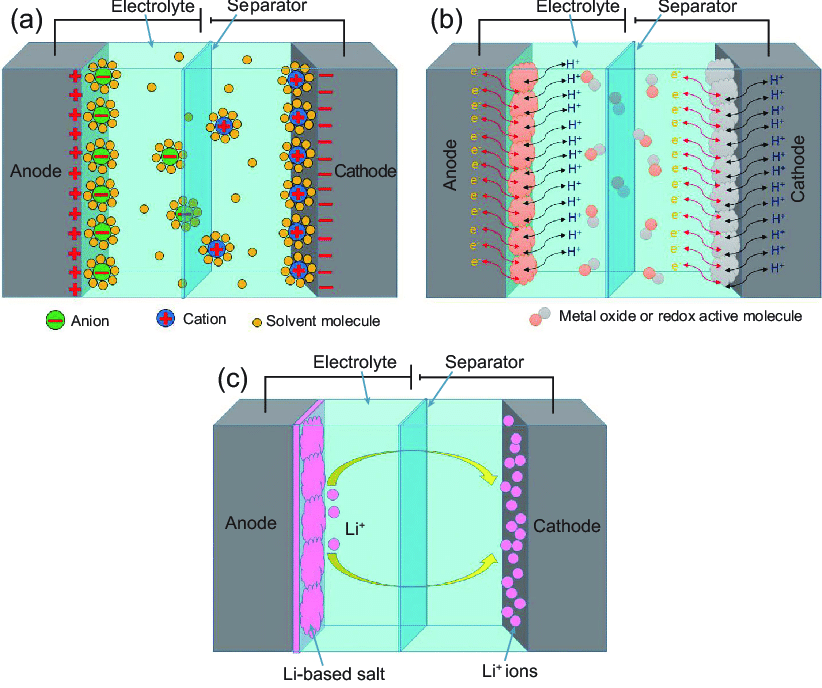
\includegraphics[width=0.50\columnwidth]{Imágenes/Diagrama esquemático de supercapacitores.png}
  \caption{Diagramas esquemático de los distintos tipos de supercapacitores. (a) EDLC (b) Pseudocapacitor (c) Híbrido.}
  \label{ragone}
\end{figure} 


\subsection{Aplicaciones}

Los supercapacitores son deseados en aplicaciones en donde es necesaria una gran cantidad de potencia en una ventana de tiempo pequeña. Algunos ejemplos de estas aplicaciones son:

\subsubsection{Búfer de energía para equipos de baja potencia}

Los supercapacitores pueden utilizarse como una fuente de energía de respaldo para RAM, SRAM y microcontroladores en el caso de un apagado de emergencia. Las UPS (del inglés \emph{uninterruptible power supplies}, sistemas de alimentación ininterrumpida) pueden ser alimentadas por supercapacitores, los cuales reemplazarían bancos de capacitores electrolíticos con mayores dimensiones físicas, y poseen un menor costo por ciclo, entre otras características que favorecen económicamente el uso de estos dispositivos.

\subsubsection{Microrredes}

Debido a que las microrredes generalmente son alimentadas con energía limpia y renovable, su producción no es constante a lo largo del día, y puede no llegar a igualar la demanda. El rol de los supercapacitores en una microrred en estos casos sería inyectar potencia en forma casi instantánea cuando la demanda es alta y la producción es baja. En esta situación, los supercapacitores actúan de forma óptima como búfer en conjunto con baterías químicas (como por ejemplo, baterías de litio).

En todas estas aplicaciones y debido a sus bajos niveles de tensión, los supercapacitores son utilizados en \emph{arreglos} o \emph{bancos} para poder satisfacer los requerimientos de cada aplicación, los cuales pueden ser de tensión, corriente o energía eléctrica.

\subsection{Bancos de supercapacitores}

Un banco de supercapacitores se define como un arreglo de supercapacitores, agrupados de forma de poder ser incluidos en sistemas de mayor potencia, y satisfacer ciertos requerimientos que un solo supercapacitor no podría cumplir. Observando las ecuaciones de capacidad equivalente para distintos arreglos:

\begin{itemize}
  \item Capacitor equivalente en serie:
  \begin{equation}
    \frac{1}{C_{eq}} = \sum_{n=1}^{N} \frac{1}{C_i}
    \label{cap-serie}
  \end{equation}
  \item Capacitor equivalente en paralelo:
  \begin{equation}
    C_{eq} = \sum_{n=1}^{N} C_i
    \label{cap-paralelo}
  \end{equation}
\end{itemize}

Dado que los valores de tensión que se manejan en sistemas de potencia son más elevados que los valores de tensión nominales de un solo supercapacitor, se coloca el número de elementos en serie que sea necesario hasta alcanzar el nivel de tensión requerido. Debido a que esto conlleva una disminución de la capacitancia del sistema, como puede observarse en la Ecuación \ref{cap-serie} el arreglo utilizado para este trabajo consiste en un arreglo conformado por celdas tanto en paralelo como en serie para contrarrestar este efecto indeseado \cite{fornaro}.

\subsubsection{Inconvenientes}

En supercapacitores que presentan elevados valores de capacidad, pequeños valores de tolerancia representan grandes variaciones de energía, y dentro de un mismo sistema, estas ligeras variaciones pueden significar la ruptura del material que aísla las cargas en un supercapacitor.

Uno de los primeros efectos que puede verse en un supercapacitor que trabaja por encima de su valor nominal es la evaporación interna de los materiales que componen el electrolito, generando un aumento de la presión dentro del dispositivo capaz de provocar un estallido, destruyendo el encapsulado y poniendo el riesgo la salud del operario. Para esto es necesario conocer los valores a los cuales trabajarán en un determinado sistema tanto el banco completo de supercapacitores como cada supercapacitor individualmente, y tener dichos valores controlados en pos de un sistema eficiente y seguro.

Es por este motivo que en el diseño del banco de supercapacitores se debe implementar un método de control en las tensiones de cada celda, ya que si nos encontramos con que una de las celdas tiene un bajo valor de capacidad respecto de las otras, éstas tendrán un alto valor de tensión en estado estacionario pudiendo sobrepasar la tolerancia máxima, culminando en la destrucción del sistema completo. 

El banco de supercapacitores disponible en el instituto, y utilizado en este trabajo, posee un esquema de balanceo empleando transistores MOSFET, el cual es explicado a continuación.

\subsubsection{Método de balanceo mediante MOSFET}

Este control supone emplear las llaves MOSFET colocadas en paralelo con cada juego de supercapacitores. Las mismas aumentan su corriente exponencialmente a medida que aumenta la tensión del supercapacitor. En la Figura \ref{balanceo-mosfet} puede observarse un diagrama del método.

Tiene un manejo más eficiente de la energía, debido a que con baja tensión en el supercapacitor, los valores de corriente a través de la llave son extremadamente bajos, y al llegar el supercapacitor a un estado de carga determinado, los valores de corriente a través de la llave contribuyen para ir progresivamente balanceando el conjunto de celdas, y llegar al estado de carga sin tener que descargar elevados valores de corriente.

\begin{figure}[hbt!]
  \centering
  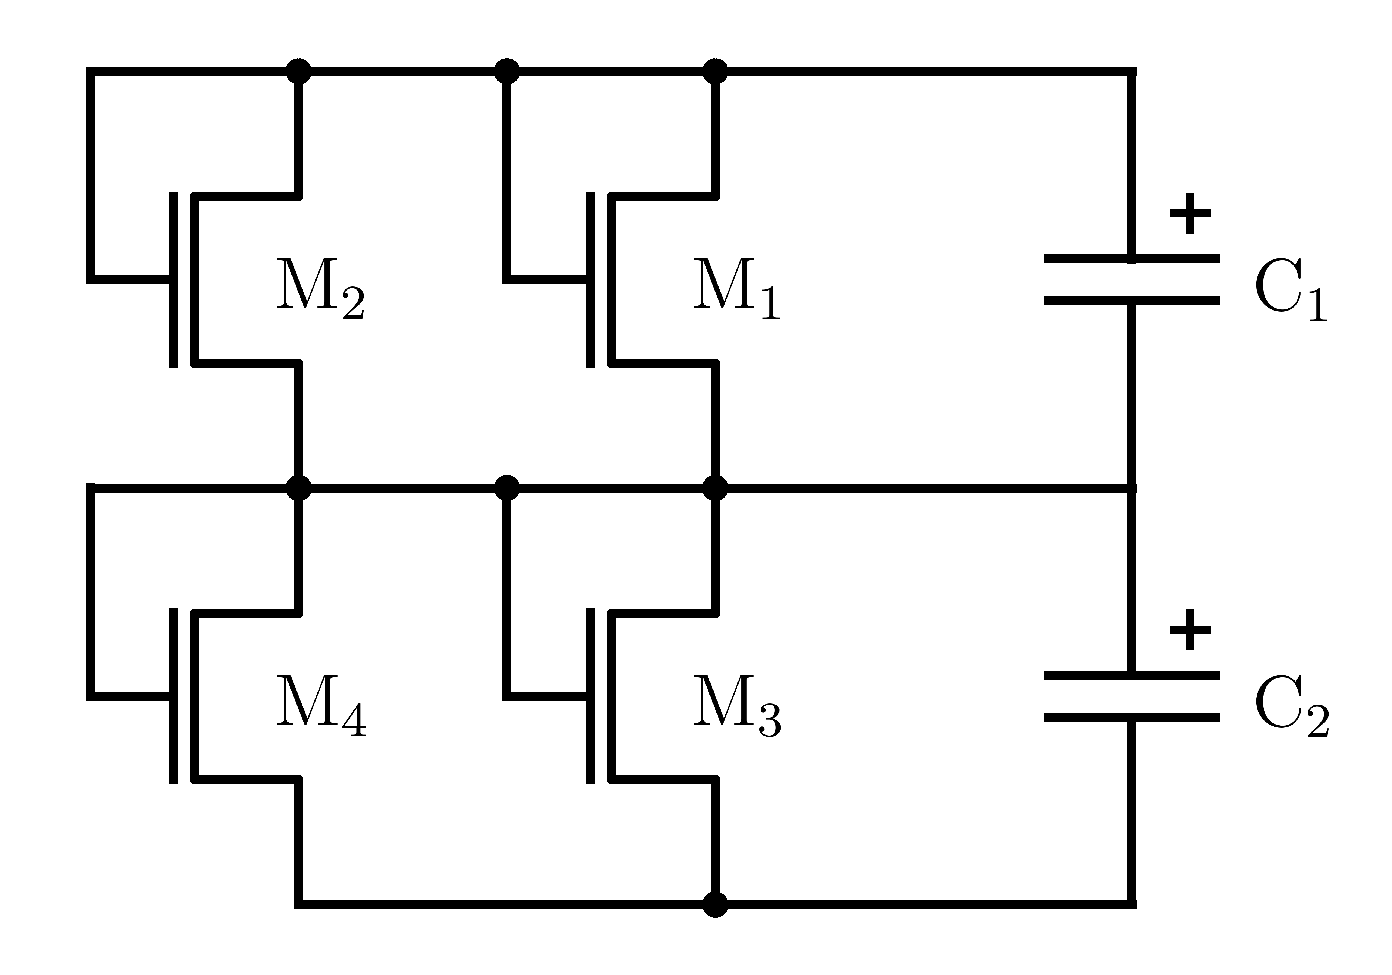
\includegraphics[width=0.40\columnwidth]{Imágenes/Balanceo por MOSFET.pdf}
  \caption{Diagrama circuital del balanceo mediante MOSFET.}
  \label{balanceo-mosfet}
\end{figure} 

En resumen, este método emplea MOSFET como resistencias variables para balancear los supercapacitores. De esta forma, si algún supercapacitor comienza a elevar su tensión respecto del resto de los elementos del banco, entonces su resistencia de descarga será menor, compensando selectivamente las diferencias en el banco.

\section{Baterías de ión de litio}

\subsection{Principio básico de funcionamiento}

Los reactivos en las reacciones electroquímicas de una celda de Li-Ión son el ánodo y cátodo, los cuales contienen átomos de litio. Durante la carga, iones $\text{Li}^+$ son generados por el electrodo positivo (el cual funciona como ánodo en este proceso), migran a través del electrolito y el separador poroso, y penetran el electrodo negativo (el cual funciona como cátodo), mientras los electrones circulan por el circuito externo. En el proceso, el electrodo positivo se oxida perdiendo electrones, y el electrodo negativo es reducido (reacción \emph{redox}) capturando electrones.

\subsection{Características constructivas}

La gran ventaja de la tecnología de litio proviene del hecho de que Li es un metal liviano, y es el elemento más electropositivo\footnote{La tendencia de un átomo de donar electrones y formar cationes positivamente cargados.} que se encuentra en la naturaleza (lo que hace que la tensión de sus baterías sea significativamente más alta que la de otras tecnologías). Además las baterías de Li-Ión son de bajo mantenimiento, lo cual es una ventaja que otros tipos de tecnología, como por ejemplo las baterías a base de níquel, no poseen. Las baterías de ión de litio pueden usar diferentes materiales como electrodos:

\begin{itemize}
  \item La combinación más común es un cátodo de \textbf{óxido de litio cobalto} y un ánodo de \textbf{grafito}, utilizado mayormente en dispositivos electrónicos portables como celulares y notebooks.
  \item Otros materiales utilizados para el cátodo se tratan de \textbf{dióxido de litio-manganeso}, utilizado en automóviles híbridos y eléctricos, y \textbf{litio-ferrofosfato}.
\end{itemize}

Las baterias de litio utilizan ésteres (un tipo de compuesto orgánico) como electrolito. En el instituto se encuentran disponibles baterías de litio-ferrofosfato, las cuales se describen de forma más extensa a continuación.

\begin{figure}[hbt!]
  \centering
  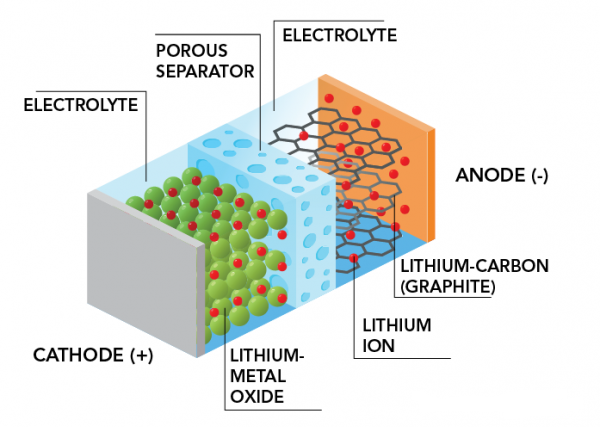
\includegraphics[width=0.47\columnwidth]{Imágenes/Partes de una batería.png}
  \caption{Partes de una batería de ión-litio.}
  \label{bateria}
\end{figure} 

\subsection{Baterías de litio-ferrofosfato}

Las baterías de litio-ferrofosfato (LiFePO$_4$ o LFP) son un tipo de baterías de Li-Ión que utilizan litio-ferrofosfato como material de cátodo, y grafito con respaldo metálico como ánodo. La densidad másica de energía en una batería LFP es menor que la de otros tipos de baterías Li-Ión, y también posee una tensión nominal menor. Aún así, debido a su bajo costo, baja toxicidad (no posee cobalto), largo ciclo de vida y otros factores, las baterías LFP se están utilizando cada vez más en vehículos, aplicaciones estacionarias a gran escala, y sistemas de energía de emergencia.

Un ejemplo de este emergente uso de las baterías LFP se da en una de las empresas automotoras y de energía limpia más novedosas del mundo, \emph{Tesla}, la cual anunció que cambiará las baterías de óxido de níquel-cobalto-aluminio (NCA), utilizadas en sus vehículos y aplicaciones estacionarias (como por ejemplo, el \emph{Megapack} de la Figura \ref{megapack}), por este tipo de tecnología.

\begin{figure}[hbt!]
  \centering
  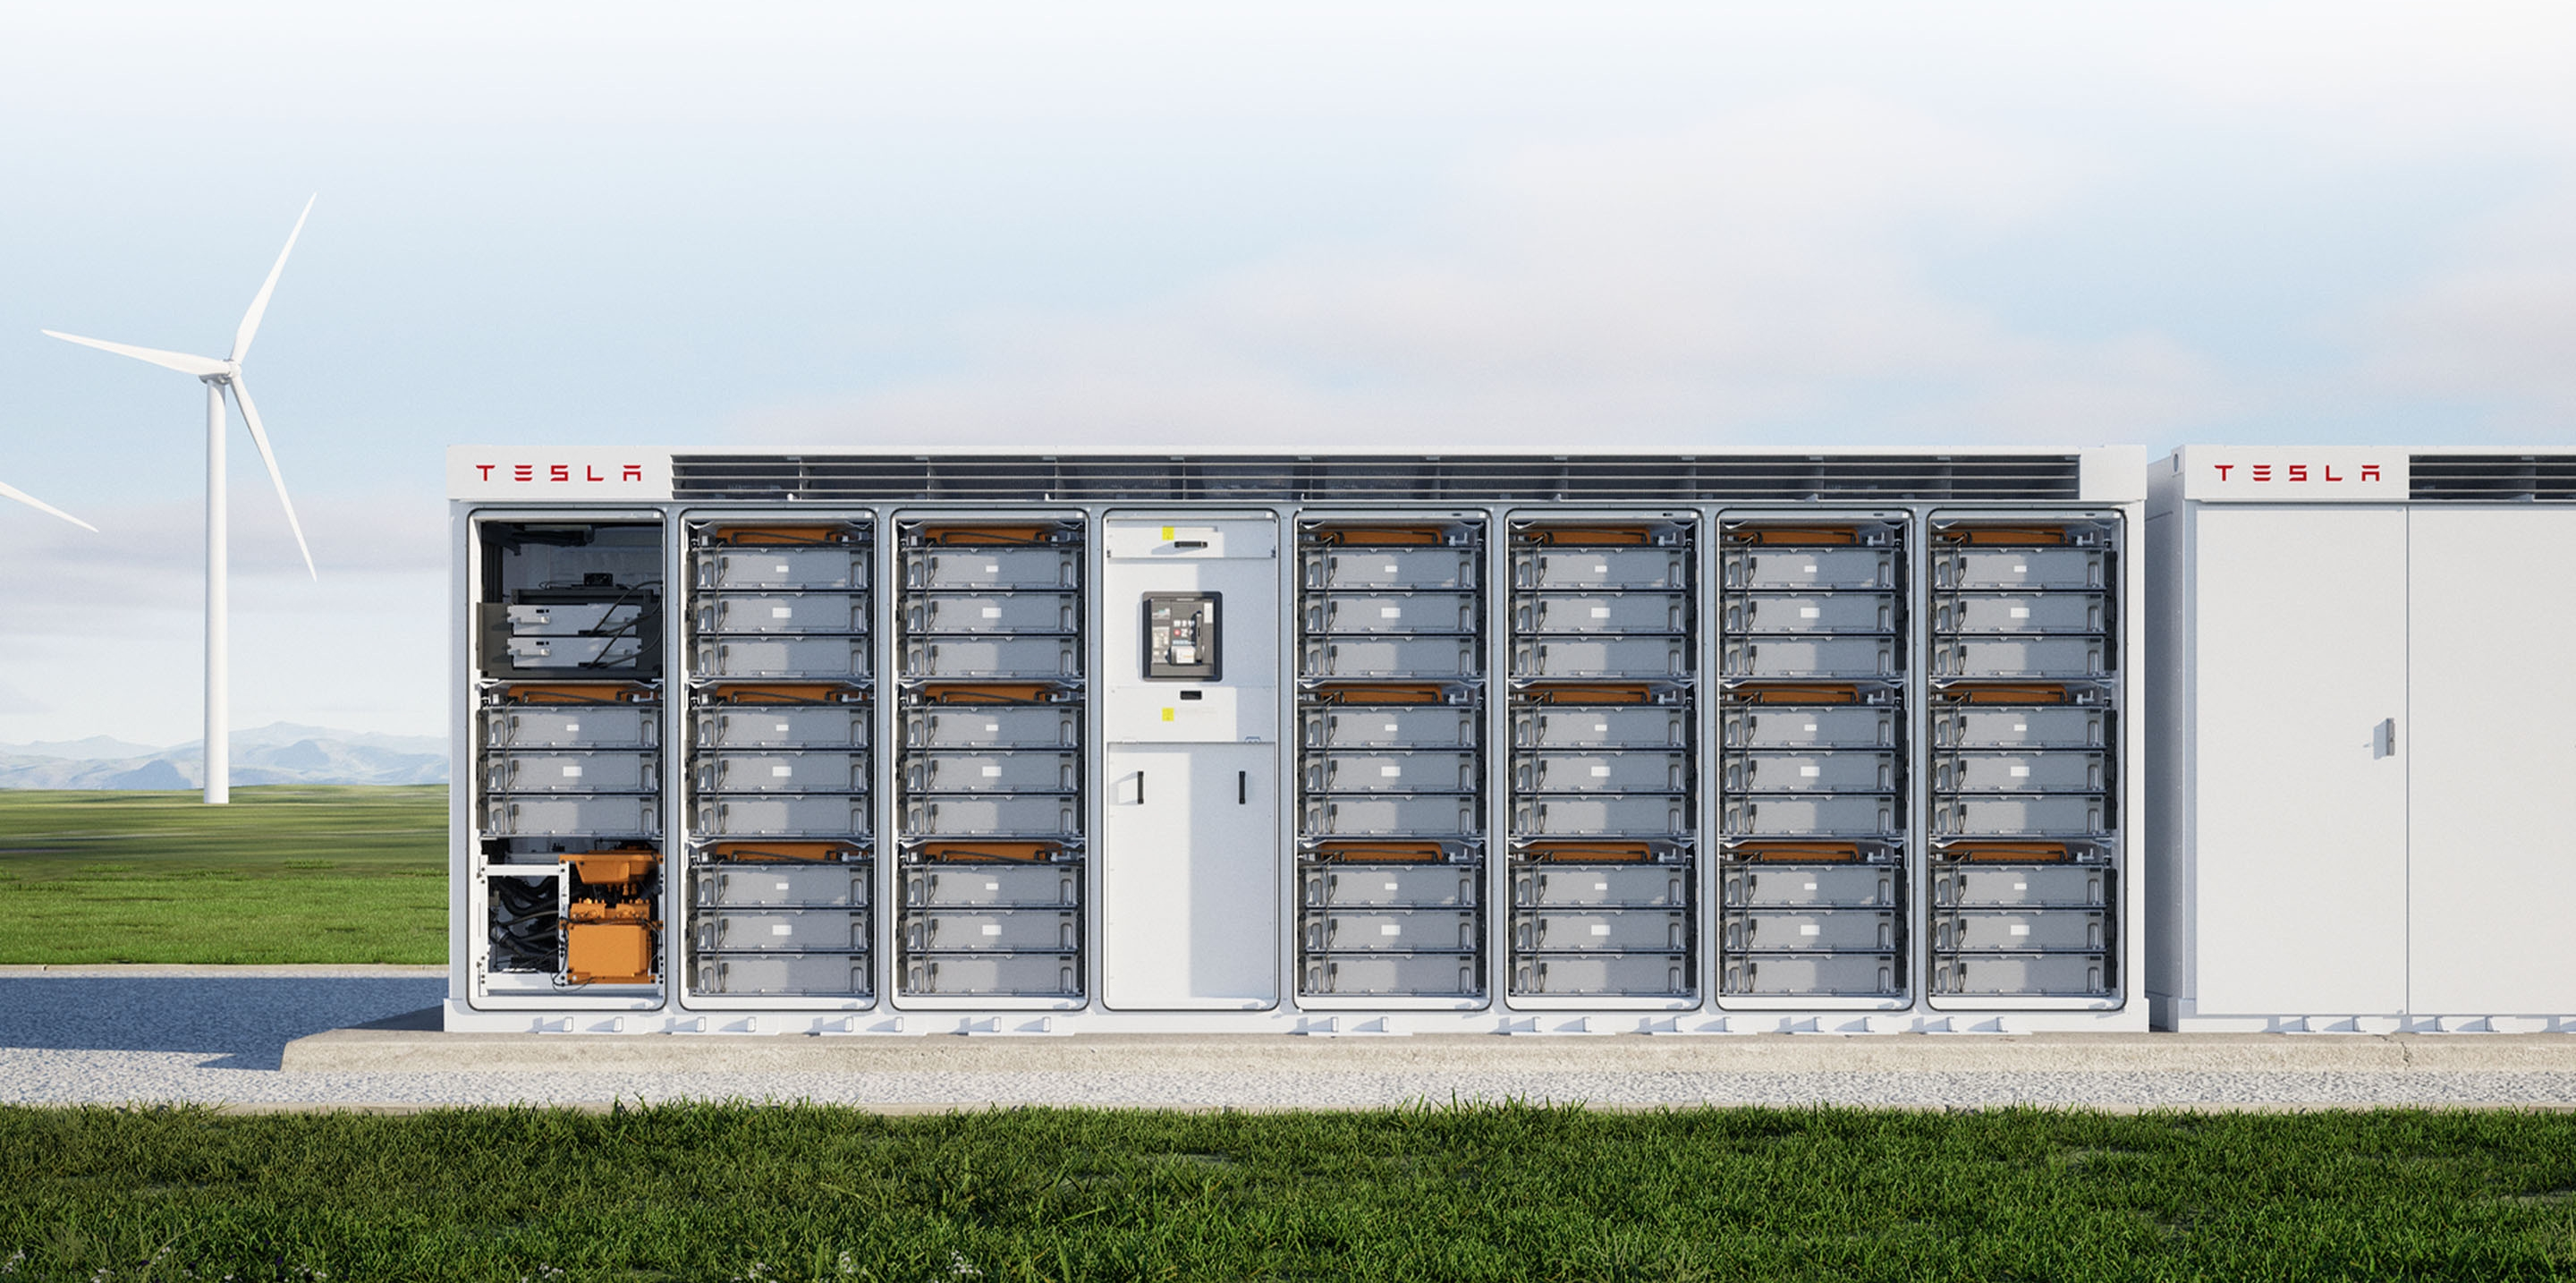
\includegraphics[width=0.65\columnwidth]{Imágenes/Tesla Megapack.jpg}
  \caption{Megapack de Tesla, un producto estacionario de almacenamiento de energía a gran escala.}
  \label{megapack}
\end{figure} 

\subsection{Proceso de carga y descarga}

El proceso de carga para una batería de Li-Ión, la cual está compuesta de un grupo de celdas en serie, se divide en tres etapas:

\begin{enumerate}
  \item Durante la etapa de \textbf{corriente constante} (CC), el cargador aplica una corriente continua a la batería, con una tensión con tasa de aumento constante, hasta que el límite de tensión por celda es alcanzado.
  \item En la etapa de \textbf{balanceo}, el cargador reduce la corriente de carga mientras que el estado de carga (siglas SoC, del inglés \emph{state of charge}) de las celdas individuales es llevado al mismo nivel por el circuito de balanceo, llamado BMS (del inglés \emph{battery management system}). Las técnicas para lograr este balanceo varían de cargador en cargador.
  \item Finalmente, en la fase de \textbf{tensión constante}, el cargador aplica un voltaje igual a la tensión nominal de las celdas multiplicado por la cantidad de celdas en series que posee la batería, mientras la corriente disminuye gradualmente hacia cero hasta un cierto umbral especificado por el cargador. 
\end{enumerate}

El electrolito y el circuito externo proveen conducción de los elementos, pero no participan de la reacción electroquímica.

Durante la descarga, los electrones fluyen desde el electrodo negativo (ánodo) hacia el electrodo positivo (cátodo) a través del circuito externo. La reacción durante la descarga reduce el potencial químico de la celda, y por lo tanto este proceso transfiere energía de la celda a donde se disipe la energía (en gran parte el circuito externo).

Ambos electrodos permiten a estos iones de litio entrar y salir de sus estructuras a través de un proceso llamado \emph{inserción}\footnote{La inserción, también llamada intercalación, es la inclusión reversible de una molécula o ión en materiales con estructura laminar o en capas.} o \emph{extracción}, respectivamente. En la Figura \ref{bateria} puede observarse la estructura de una batería de Li-Ion, en donde se identifican el cátodo, ánodo, electrolito, y el separador poroso.

\subsection{Aplicaciones}

\subsubsection{Autos eléctricos}

La electrificación de los vehículos esta aumentando a una tasa cada vez más rápida, debido a que existen varias ventajas en utilizar trenes motrices eléctricos, comparado con los motores de combustion interna, para aplicaciones automóviles. La primer ventaja es que los dispositivos eléctricos pueden alcanzar una eficiencia de energía mucho más alta que los motores de combustión interna. La segunda ventaja es un derivado del \emph{freno regenerativo} en donde una batería recargable es instalada en un sistema, y almacena energía cinética convirtiéndola en energía eléctrica, aumentando la eficiencia \cite{evs&hevs}.

Además, estos sistemas eléctricos pueden aprovechar un gran abanico de fuentes de energía, desde centrales termoeléctricas, hasta tecnologías de energía renovable como celdas fotovoltáicas o turbinas eólicas (Figura \ref{hev}).

\begin{figure}[hbt!]
  \centering
  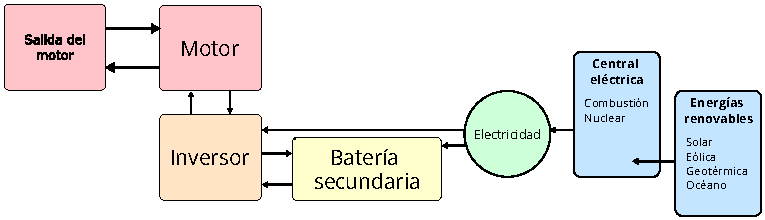
\includegraphics[width=0.65\columnwidth]{Imágenes/Flujo de la energía en un HEV.pdf}
  \caption{Flujo de la energía en un vehículo eléctrico.}
  \label{hev}
\end{figure}

\subsubsection{Almacenamiento de energías renovables}

Este tipo de baterías también puede ser utilizadas para solucionar el problema de la fluctuación de fuentes de energías renovables, como la energía solar o eólica. Además de la extensión de la red eléctrica y el desarrollo de soluciónes de gestión del lado de la demanda, el almacenamiento de energía es crucial para lograr un sistema eléctrico basado principalmente en energías renovables \cite{storage}. 

Un ejemplo de esta situación se da en Alemania. En 2011, las energías renovables ya aportaban aproximadamente el 20\% de la producción de energía eléctrica. En 2012, los sistemas fotovoltáicos lograron en los primeros seis meses una participación del 5.1\%, mientras que los generadores éolicos una participación del 8.9\% de la energía eléctrica total producida. Los primeros días de agosto del 2012, la energía solar alcanzó una producción de \SI{31}{\giga\watt} sobre la capacidad instalada, y la energía eólica un valor de más de \SI{29}{\giga\watt}. Por el momento, el acta de energías renovables de Alemania preveé que la tarifa de alimentación\footnote{Subvención estatal creada para acelerar el desarrollo de fuentes de energías renovables, a través de la provisión de un precio garantizado por encima del mercado para productores.} para sistemas fotovoltáicos será garantizada hasta que un nivel de \SI{52}{\giga\watt} sea alcanzado. Tomando en cuenta que la curva de carga de Alemania varía solamente entre \SI{45}{\giga\watt} y \SI{85}{\giga\watt}, resulta evidente que un incremento de energías renovables solo puede ser dado si un sistema de almacenamiento es implementado \cite{alemania}.

\begin{figure}[hbt!]
  \centering
  \subfloat[Fuentes de generación de energía en Alemania.]{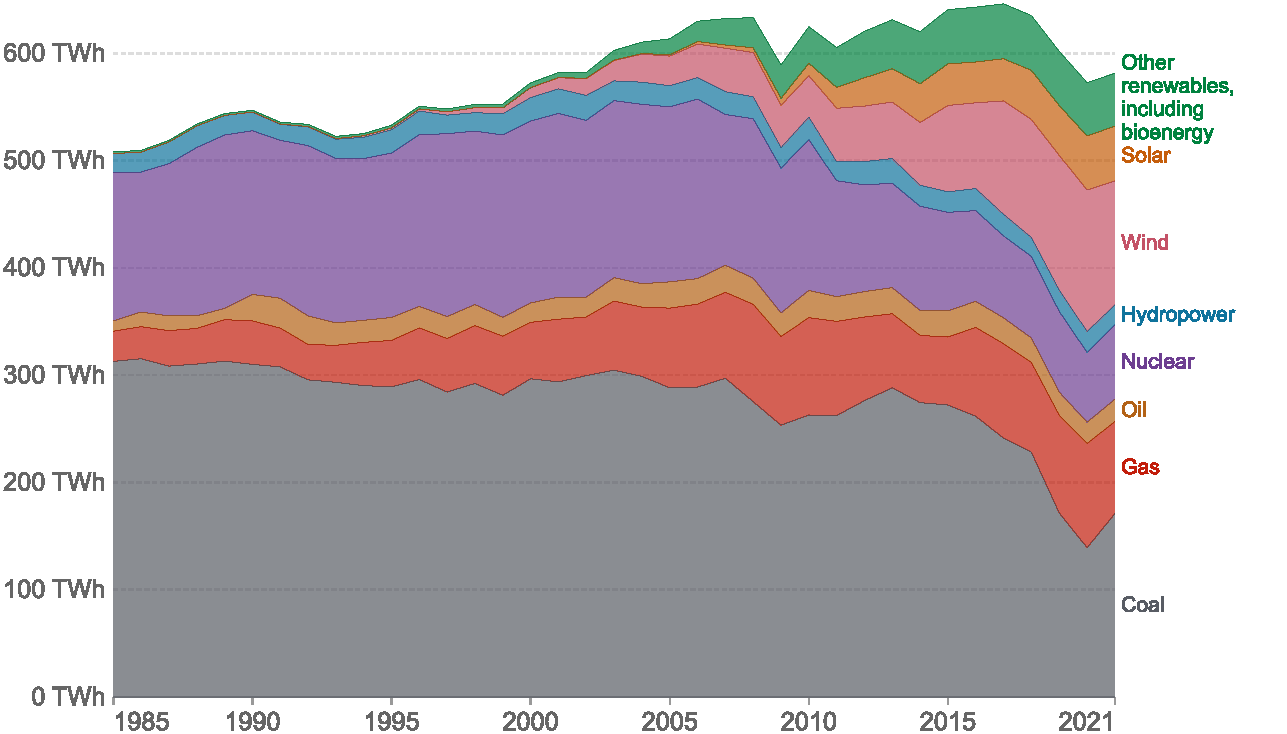
\includegraphics[width=0.45\textwidth]{Imágenes/Generacion de energía en Alemania.pdf}}    
  \hspace{3.5mm}
  \subfloat[Porcentajes de aporte de cada fuente de generación.]{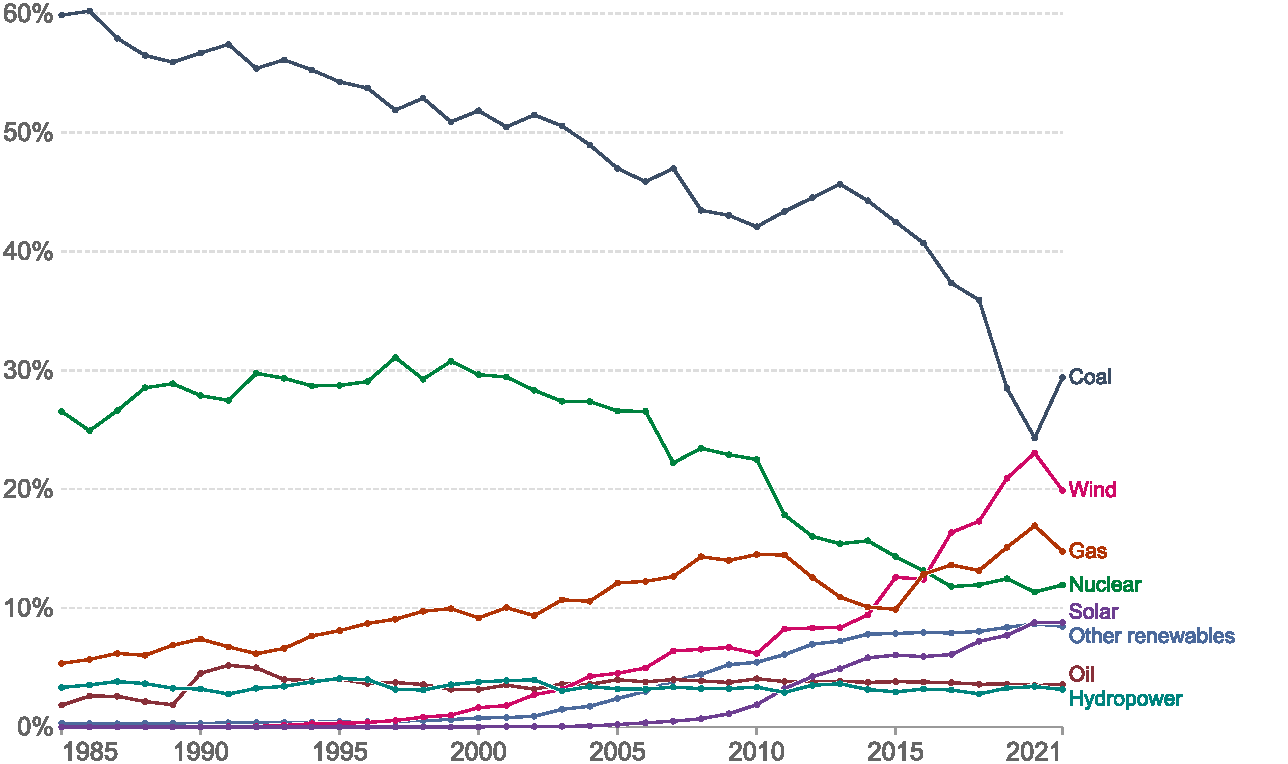
\includegraphics[width=0.45\textwidth]{Imágenes/Generacion de energía en Alemania en porcentaje.pdf}}
  \caption{Curvas de crecimiento de la generación de energías renovables.}
  \label{generacion-alemana}
\end{figure}

Por lo tanto, estos módulos de almacenamiento de energía son requeridos a distintos tamaños y con distintos fines, siendo algunos instalados en forma descentralizada (por ejemplo, en combinación con sistemas fotovoltáicos para aumentar su tasa de autoconsumo).

\subsubsection{Sistemas de potencia satelitales}

Los sistemas de potencia de satélites se han desplazado progresivamente hacia la tecnología de ión-litio desde los principios de los 2000s.  

A medida que el peso se convirtió en una cuestión clave de diseño para los satélites, la gran densidad másica de energía provista por la tecnologia Li-Ión aceleró su adaptación al principio de este siglo. Muy rápidamente, la transición ocurrió para los satélites de las órbitas geoestacionarias GEO (del inglés \emph{geostationary earth orbit}), órbita terrestre baja LEO (del inglés \emph{low earth orbit}) y la órbita terrestre media MEO (\emph{medium earth orbit}) gracias a las numerosas ventajas de las baterías Li-Ión, como su baja disipación térmica, autodescarga baja, y gran eficiencia. Para los fines de 2012, más de 200 satélites fueron lanzados mundialmente utilizando esta tecnología, y más del 99\% de los contratos satelitales refieren a las baterías Li-Ión en su diseño \cite{satellites}.

\begin{wrapfigure}{r}{0.45\textwidth}
  \vspace{-10pt}
  \begin{center}
    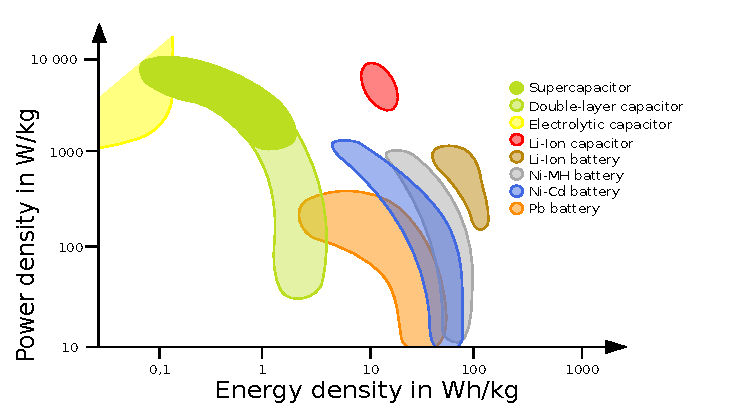
\includegraphics[width=0.44\textwidth]{Imágenes/Diagrama de Ragone.pdf}
  \end{center}
  \vspace{-15pt}
  \caption{Diagrama de Ragone.}
  \label{ragone}
\end{wrapfigure}

\subsection{Diferencias con los supercapacitores}

Como se ha visto, tanto las baterías como los supercapacitores son dispositivos de almacenamiento de carga con aplicaciones diversas, en las cuales ambos cumplen el rol de proveer energía. Sin embargo, los dos tienen características muy diferentes.

En la Figura \ref{ragone} puede observarse un diagrama de Ragone, el cual es utilizado para realizar comparaciones entre fuentes de almacenamiento. El eje horizontal indica la densidad másica de energía (en J/kg), lo que conceptualmente representa la capacidad de almacenamiento de energía. En cambio el eje vertical indica la densidad másica de potencia (en W/kg) y representa qué tan rápido puede ser entregada esa energía.

Aquí se puede observar la clara diferencia entre las baterías y los supercapacitores. Las baterías son capaces de almacenar mucha energía pero con una absorción y entrega de potencia mucho menos rápida que la de los supercapacitores. En cambio, los supercapacitores son capaces de entregar energía a una tasa órdenes de magnitud más alta, pero la cantidad de 
energía almacenada posible es limitada.

Estas diferencias pueden verse también en las aplicaciones mencionadas anteriormente para cada uno. En el caso de los supercapacitores, estos actuaban como búfer en situaciones de emergencia o con ventanas de tiempo cortas donde se requería una entrega importante de potencia. En cambio, el rol de las baterías de litio en los ejemplos dados era de almacenamiento de grandes cantidades de energía.

Es importante tener en cuenta que este diagrama no tiene en cuenta otras características intrínsecas de los módulos de almacenamiento, como su vida útil y su memoria.

\section{Sistemas híbridos de almacenamiento de energía}

Debido a sus características opuestas observadas en el diagrama de Ragone, las baterías y los supercapacitores se complementan muy bien, y por lo tanto la construcción de un sistema híbrido con ambos tipos de dispositivos presenta una gran flexibilidad a la hora de suministrar energía a aplicaciones móviles. En el caso de un sistema híbrido con baterías de litio y supercapacitores, el objetivo principal de las baterías es el de satisfacer la demanda de corriente, correspondiente a la potencia media demandada por el bus de continua \cite{estimacion}. Complementariamente, los supercapacitores son los encargados de lidiar con las variaciones abruptas de corriente que demande la carga.

La incorporación de un banco de supercapacitores en conjunto a la baterías de litio brinda además el incremento de la vida útil de la batería en un 300\%, ya que los picos de corriente serán entregados por el banco, lo que disminuye las exigencias de la batería.

Para formar este sistema híbrido, es necesario utilizar conversores electrónicos de potencia para poder ajustar los niveles de tensión de ambos dispositivos, y permitir que funcionen en conjunto. Estos tipos de conversores son analizados en el siguiente capítulo.   

\section{Resumen}

En este capítulo se desarrollaron las características de dos tipos de dispositivos que almacenan energía: los supercapacitores y las baterías de litio. Se presentaron sus mecanismos de funcionamiento, junto a algunas aplicaciones en las que se encuentran presentes.

Por último, se realizó una comparación de ambas con respecto a sus capacidades de almacenamiento de energía, y la rapidez con la que esta puede ser entregada. Este análisis de diferencias entre los dispositivos bajo estudio dió como conclusión que su operación en conjunto es capaz de formar un sistema híbrido con una gran flexibilidad bajo un amplio rango de operaciones.

\newpage

\chapter{Convertidores CC-CC}
\label{convertidores-cc-cc}

\section{Introducción}

Los convertidores electrónicos de potencia de CC-CC actúan como puentes de transferencia de energía entre fuentes y cargas, ambas de corriente continua, que no son compatibles. Un ejemplo es cuando una fuente disponible proporciona una tensión distinta a la requerida por la carga a utilizar. Por eso mismo, la función de estos tipos de  convertidores es la de adaptar tal tensión de la fuente con la máxima eficiencia posible de transferencia de energía.

Normalmente, además de la conversión de nivel de tensión de continua, los convertidores proveen una salida regulada. Dependiendo de la topología del convertidor, la tensión de salida puede ser mayor o menor a la de la entrada.

Los convertidores electrónicos de potencia pueden dividirse en lineales y conmutados. En este capítulo, se presentan los convertidores conmutados, específicamente el convertidor elevador, el cual es utilizado en este trabajo.

\section{Convertidores CC-CC conmutados}

Los convertidores conmutados son una alternativa eficiente respecto de los reguladores lineales. En un circuito de un convertidor conmutado, los transistores operan como llaves, estando completamente prendidos o completamente apagados. Asumiendo que la llave es ideal en la Figura \ref{convertidor-basico}, la salida es igual que la entrada cuando la llave está cerrada, y nula cuando la llave está abierta.

\begin{figure}[hbt!]
    \centering
    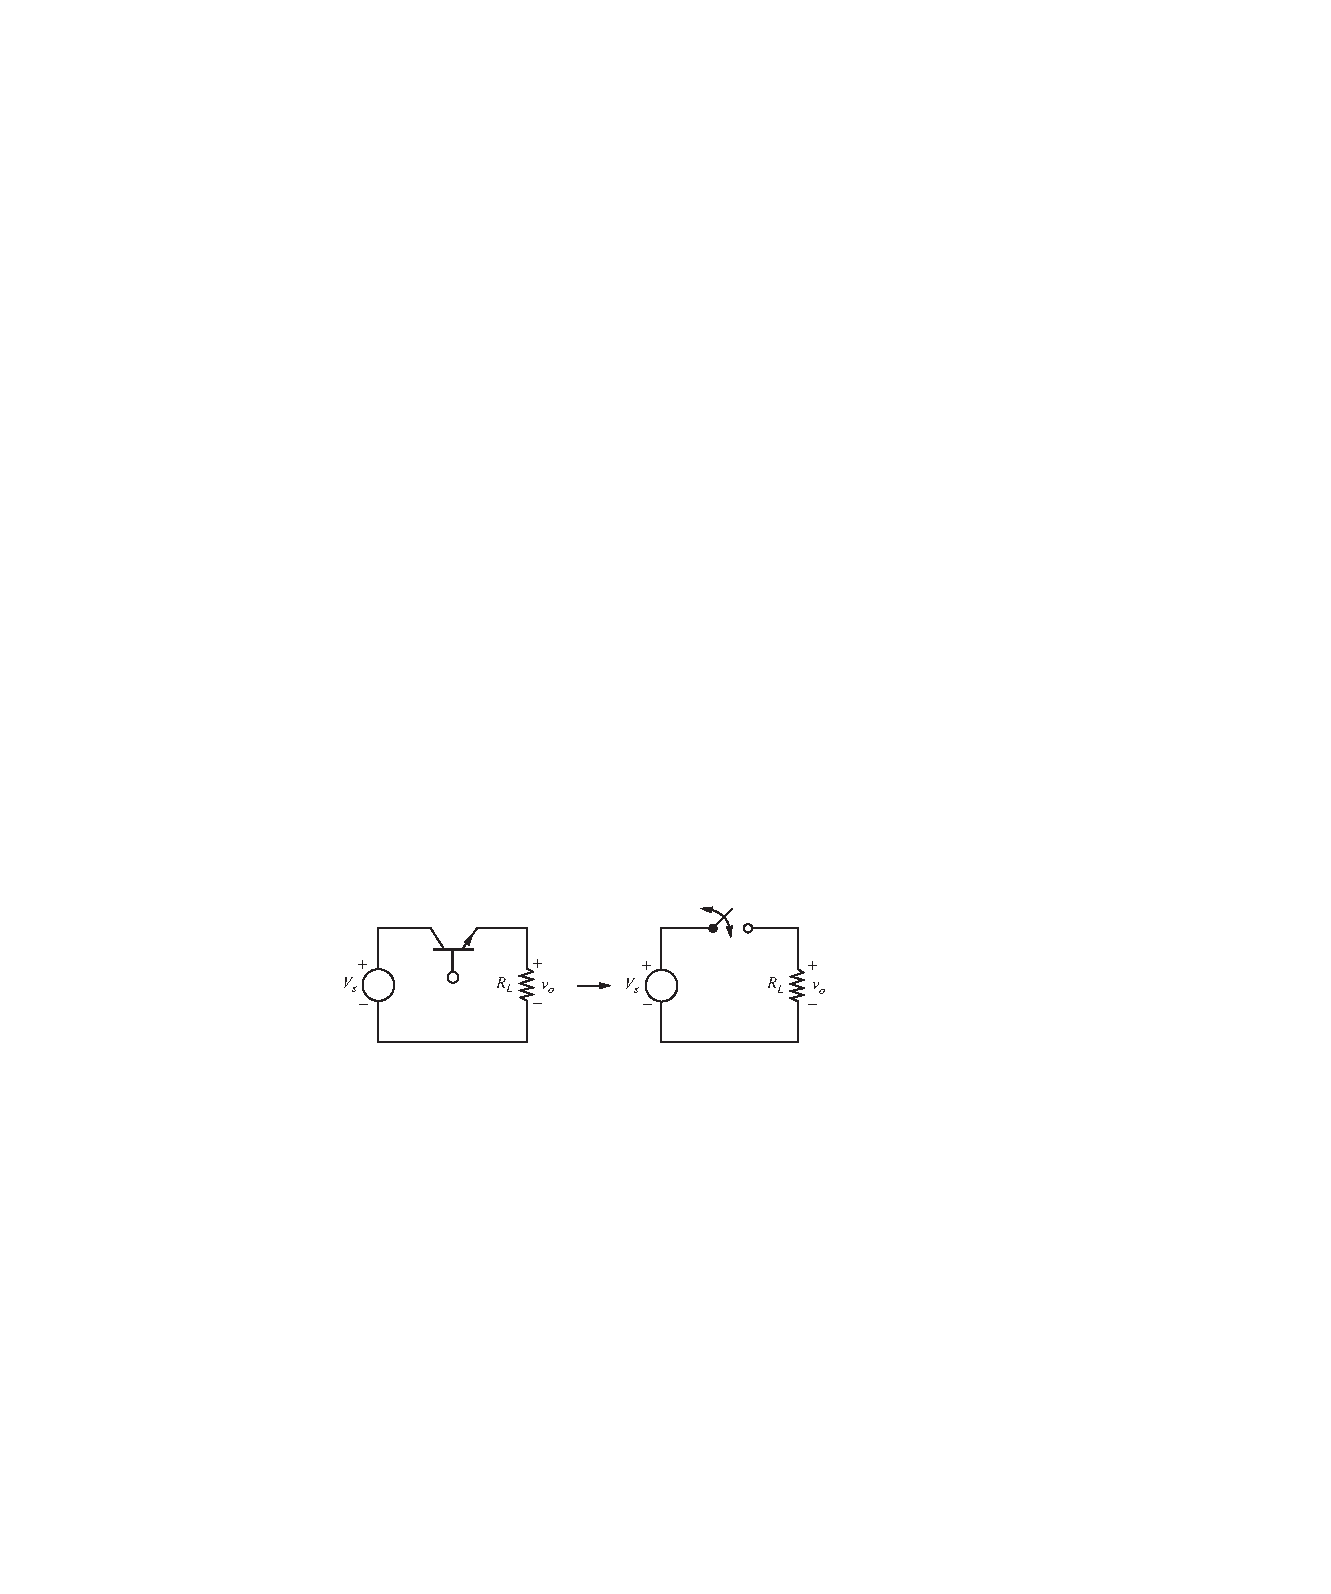
\includegraphics[width=0.55\columnwidth]{Imágenes/Convertidor conmutado básico.pdf}
    \caption{Un convertidor conmutado CC-CC básico y su equivalente de conmutación.}
    \label{convertidor-basico}
\end{figure} 

La conmutación periódica de la llave resulta en la salida en pulsos mostrada en la Figura \ref{salida-conmutador}.

\begin{figure}[hbt!]
    \centering
    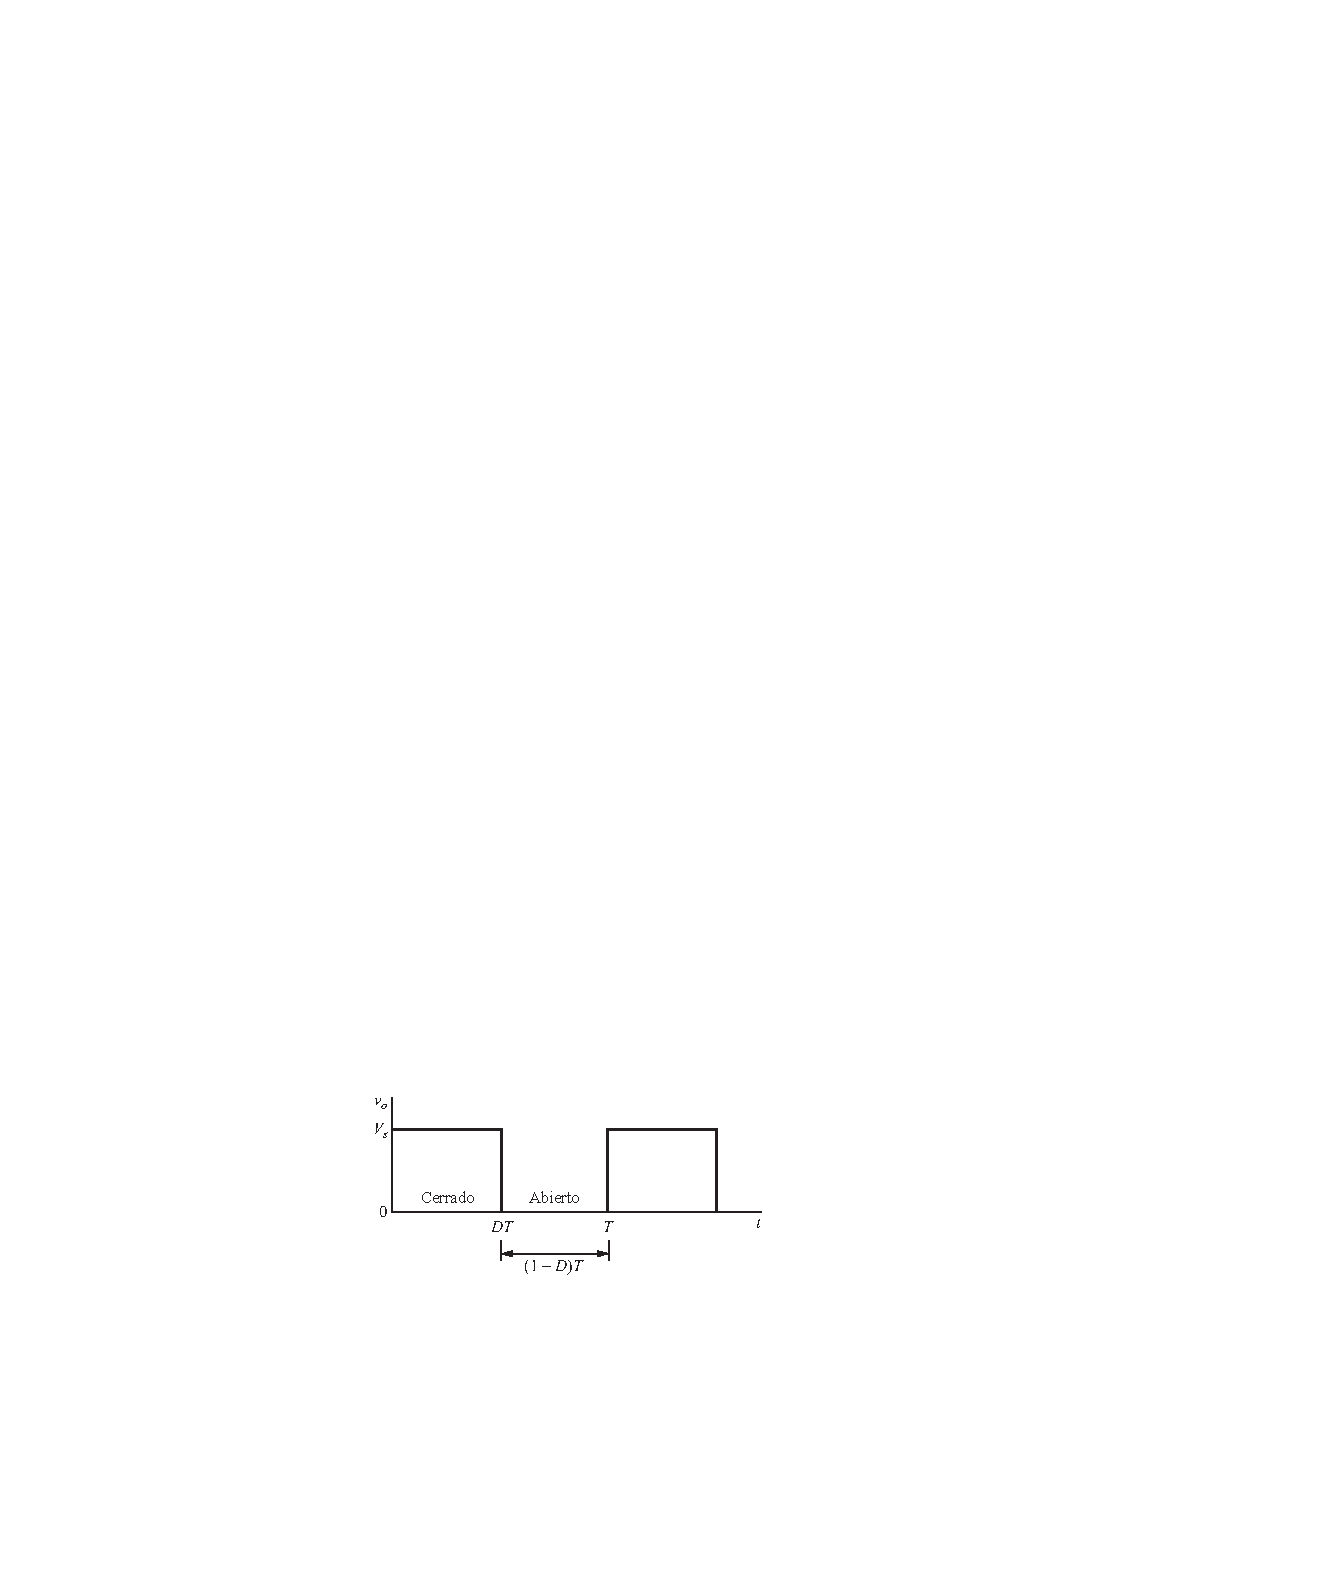
\includegraphics[width=0.55\columnwidth]{Imágenes/Salida del convertidor conmutado básico.pdf}
    \caption{Tensión de salida del circuito de la Figura \ref{convertidor-basico}.}
    \label{salida-conmutador}
\end{figure}

El valor medio de la tensión de salida es:

\begin{equation}   
    V_o = \frac{1}{T} \int_{0}^{T} v_0(t) \,dt = \frac{1}{T} \int_{0}^{DT} V_s \,dt = V_s \, D
\end{equation}

La componente de continua de la tensión de salida es controlada a través del ajuste del tiempo que la llave se encuentra cerrada respecto del período de conmutación total. Esta fracción de tiempo es llamada \emph{ciclo de trabajo} y se representa con la letra $D$.

\begin{equation}
    D \equiv \frac{t_{\mathrm{on}}}{t_{\mathrm{on}} + t_{\mathrm{off}}} = \frac{t_{\mathrm{on}}}{T} = t_{\mathrm{on}} \, f
\end{equation}

En donde $f$ es la frecuencia de conmutación. En este circuito elemental, la componente de continua de la tensión de salida siempre será menor o igual que la tensión de entrada del circuito.

Idealmente, la potencia absorbida por la llave es cero. Cuando la llave está abierta, no circula corriente por ella; cuando está cerrada, no cae tensión. Por lo tanto, toda la potencia es absorbida por la carga, y la eficiencia es del cien por ciento. Con una llave real, las pérdidas son inevitables, ya que ocurre una caída de tensión cuando está cerrada, y debe pasar por la región lineal cuando realiza la conmutación de un estado a otro.

\section{Convertidor elevador}

El convertidor elevador (\emph{boost converter} en inglés) es mostrado en la Figura \ref{convertidor-elevador}. Es llamado de tal manera ya que la tensión de salida es mayor o igual que la de entrada. Este tipo de convertidor es el utilizado para el proyecto, ya que es necesario elevar la tensión del banco de supercapacitores y las baterías de litio.

\begin{figure}[hbt!]
    \centering
    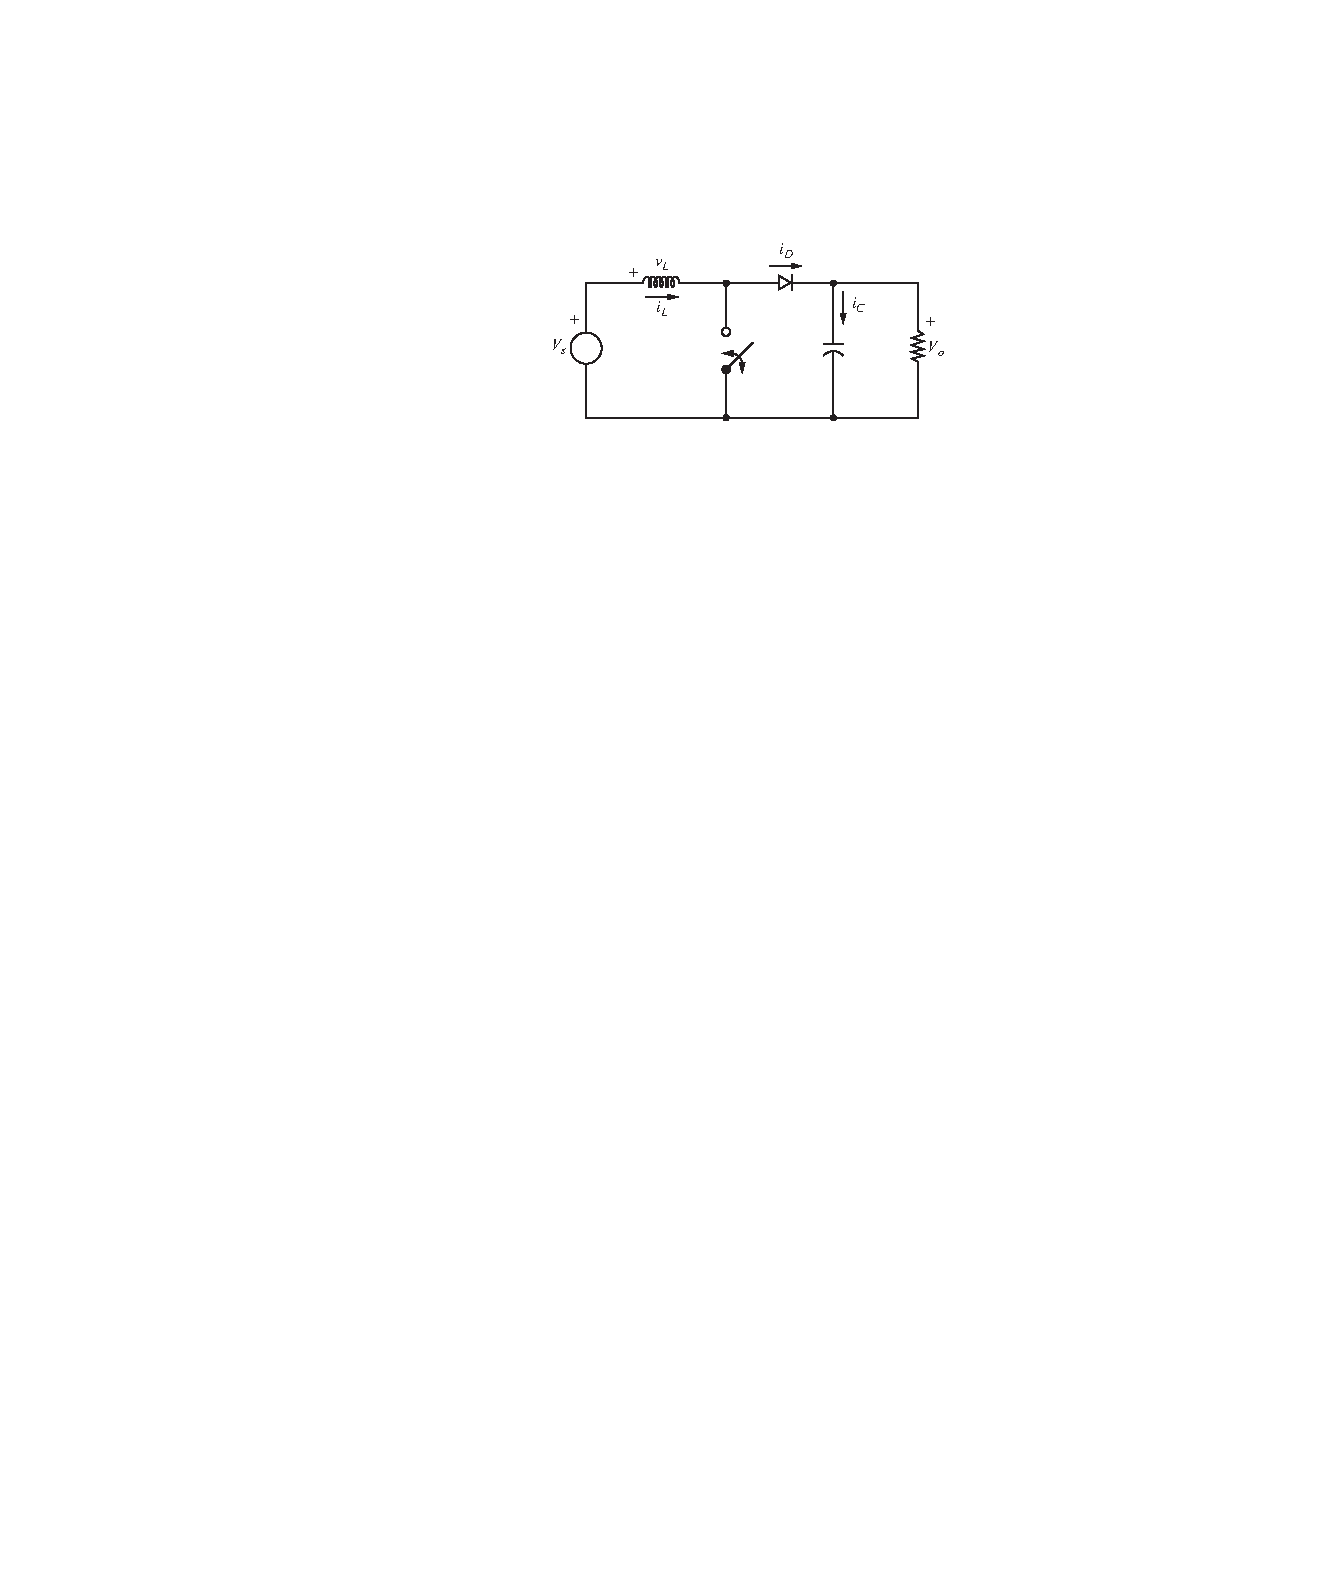
\includegraphics[width=0.55\columnwidth]{Imágenes/Convertidor elevador.pdf}
    \caption{Convertidor elevador.}
    \label{convertidor-elevador}
\end{figure}

Antes de proceder con el análisis de los modos de conducción del convertidor elevador, es necesario realizar las siguientes suposiciones:

\begin{enumerate}
    \item Existen condiciones de estado estacionario.
    \item El período de conmutación es $T$, y la llave está cerrada por un tiempo $DT$ y abierta por un tiempo $(1-D)T$.
    \item La corriente por el inductor es continua (y siempre positiva).
    \item El capacitor posee una capacitancia muy grande, y la tensión de salida es mantenida constante a un valor $V_o$.
    \item Los componentes son ideales.
\end{enumerate}

\subsection{Modo de conducción continua}

Este análisis es hecho a través de la examinación de la tensión y corriente del inductor cuando la llave está cerrada, y nuevamente cuando la llave se encuentra abierta.

\subsubsection{Análisis con la llave cerrada}

Cuando la llave se encuentra cerrada, el diodo se encuentra polarizado inversamente. La ley de Kirchhoff sobre el camino que contiene la fuente, el inductor, y la llave es:
 
\begin{equation}
    v_L = V_s = L \frac{di_L}{dt} \hspace{0.6cm} \textrm{ó} \hspace{0.6cm} \frac{di_L}{dt} = \frac{V_s}{L}
\end{equation}

La derivada de la corriente es una constante, lo que significa que la corriente incrementa linealmente cuando la llave está cerrada, como se muestra en la Figura \ref{formas-onda-elevador}b. Por lo tanto, resolviendo para la tasa de cambio de la corriente del inductor $\Delta i_L$ resulta en:

\begin{equation}
    \boxed{(\Delta i_L)_{\mathrm{cerrada}} = \frac{V_s \, D \, T}{L}}
    \label{llave-cerrada}
\end{equation}

\begin{figure}[hbt!]
    \centering
    \subfloat[Tensión en el inductor.]{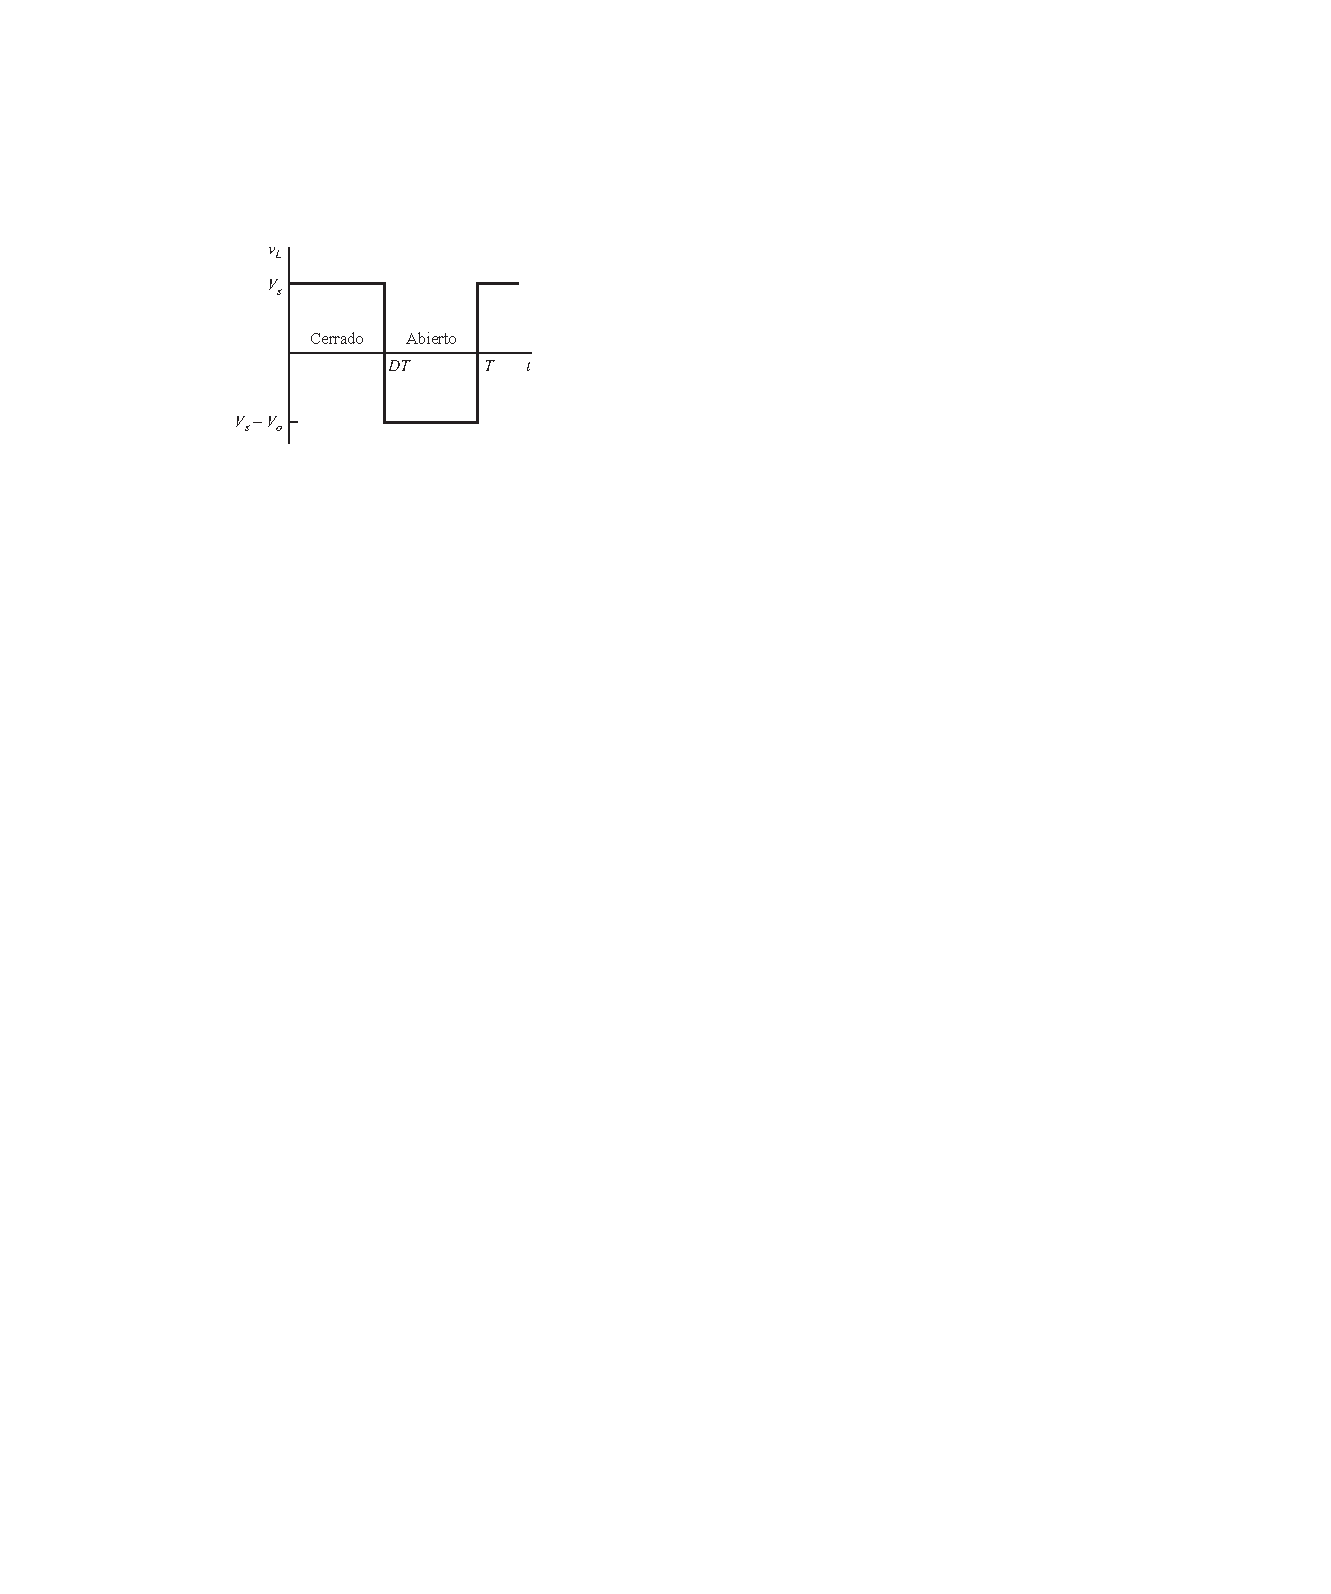
\includegraphics[width=0.38\textwidth]{Imágenes/Convertidor elevador/Tensión del inductor.pdf}}    
    \hspace{10mm}
    \subfloat[Corriente por el inductor.]{\includegraphics[width=0.38\textwidth]{Imágenes/Convertidor elevador/Corriente del inductor.pdf}}
    \hspace{10mm}
    \subfloat[Corriente por el diodo]{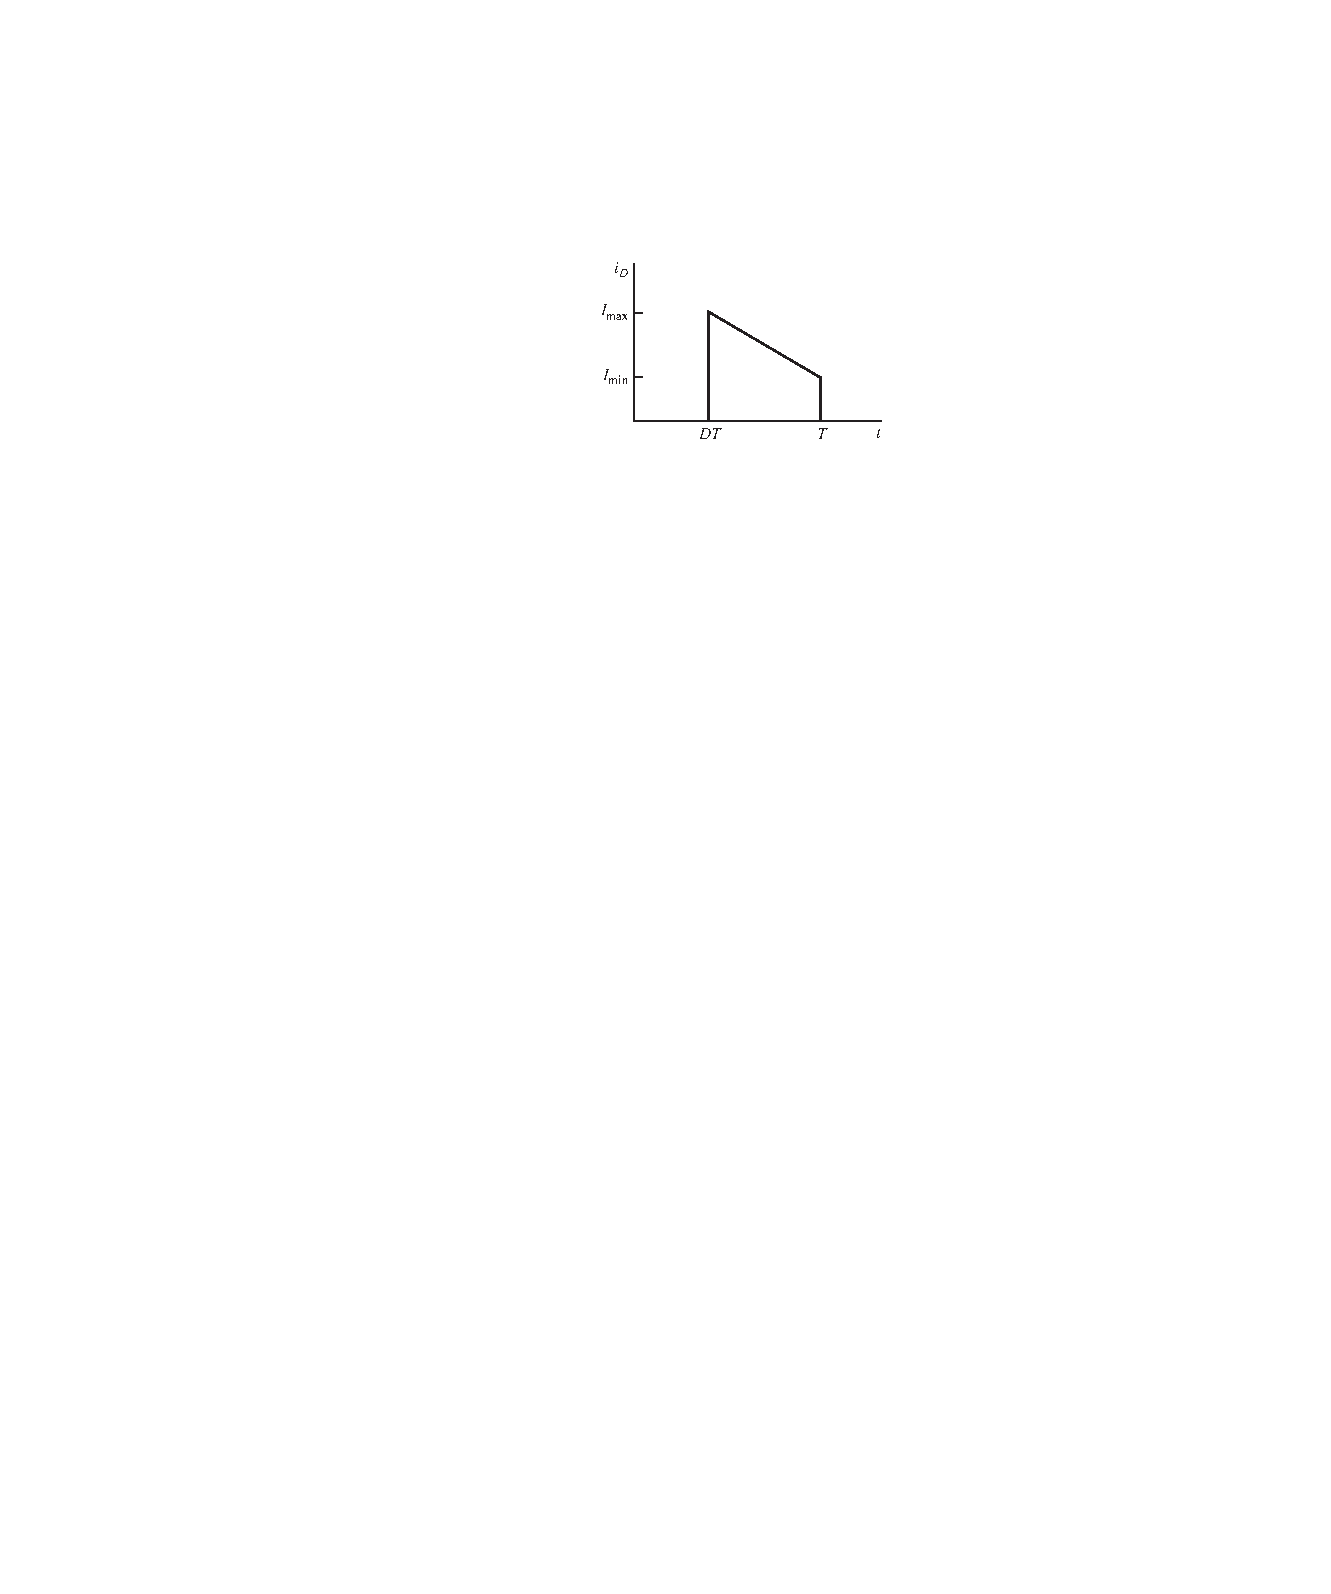
\includegraphics[width=0.38\textwidth]{Imágenes/Convertidor elevador/Corriente del diodo.pdf}}
    \hspace{10mm}
    \subfloat[Corriente por el capacitor]{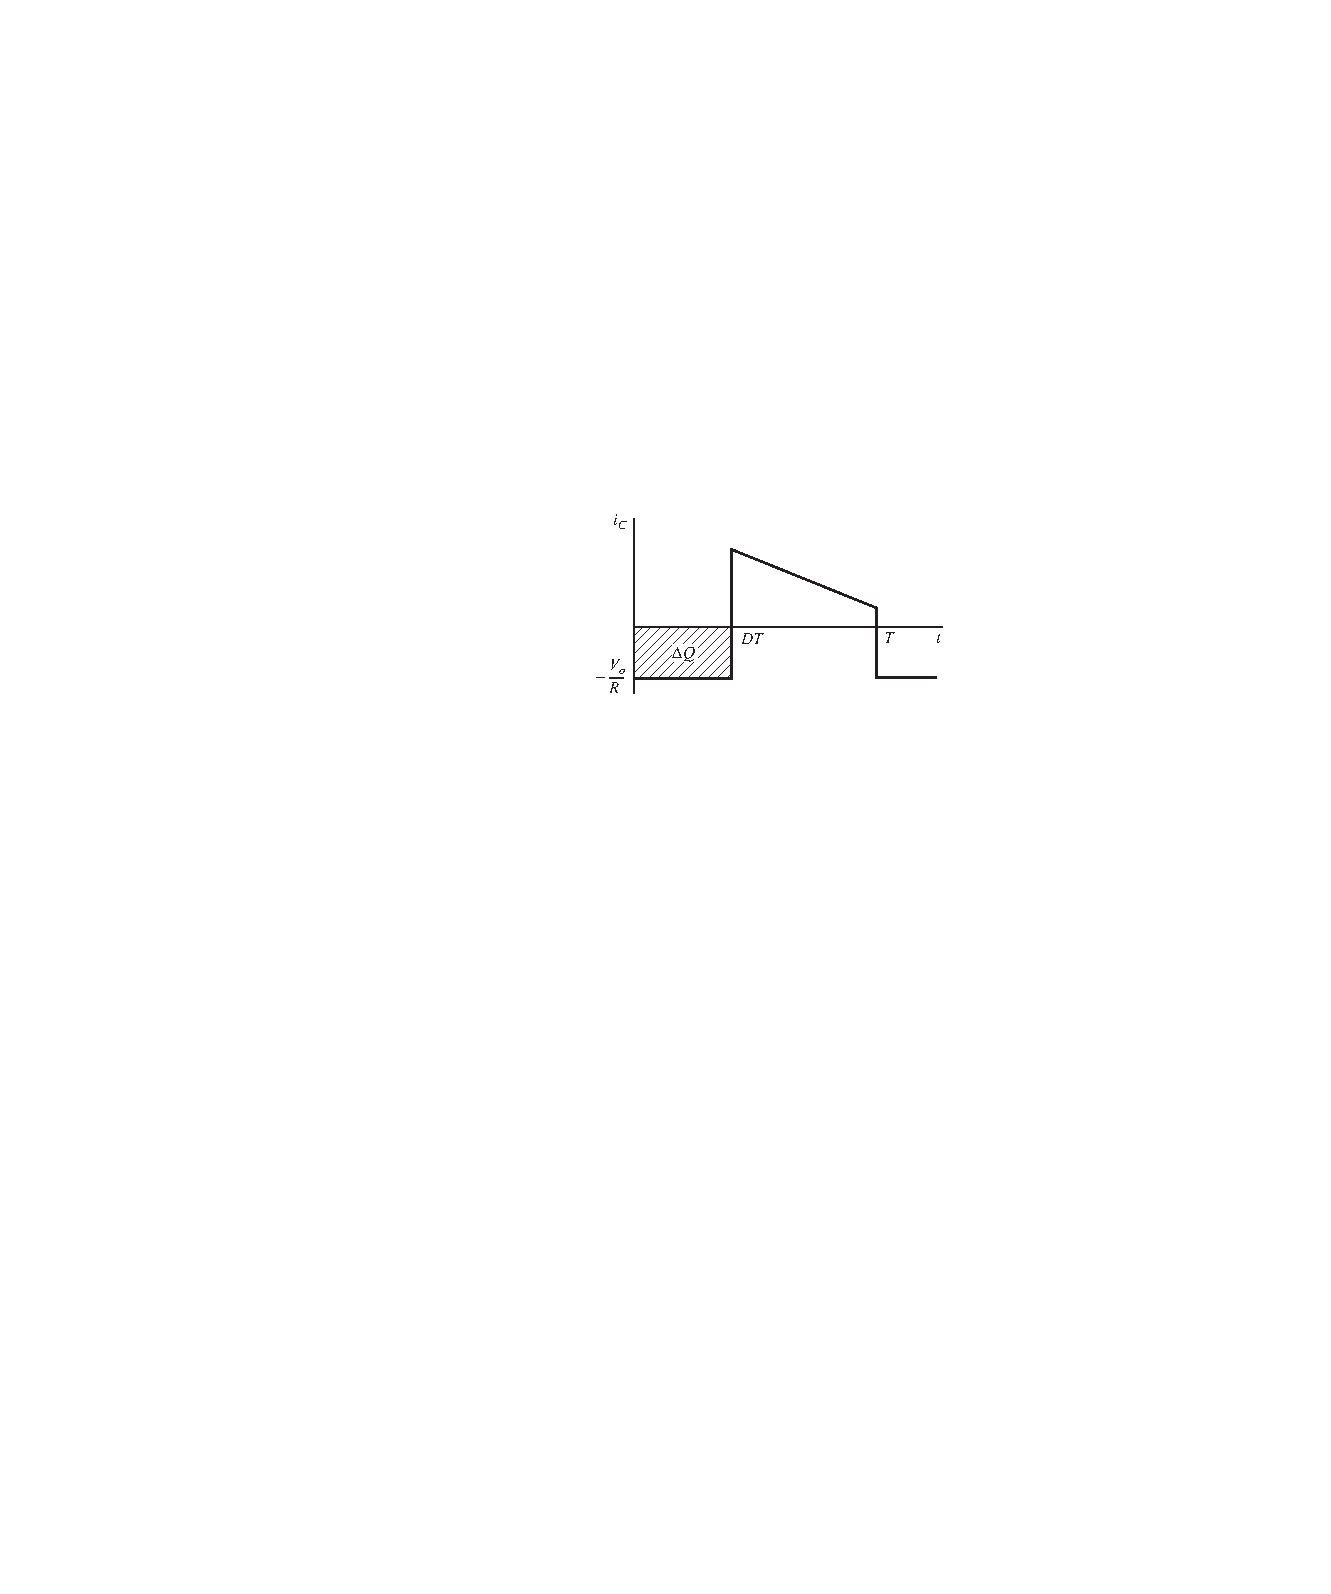
\includegraphics[width=0.38\textwidth]{Imágenes/Convertidor elevador/Corriente del capacitor.pdf}}
    \caption{Formas de onda de un convertidor elevador.}
    \label{formas-onda-elevador}
\end{figure}

\subsubsection{Análisis con la llave abierta}

Cuando la llave se abre, la corriente del inductor no puede cambiar instantáneamente, así que el diodo se polariza directamente para proveer un camino a $i_L$. Asumiendo que la tensión de salida $V_o$ es constante, la tensión que cae en el inductor es:

\begin{equation}
    v_L = V_s - V_o = L \frac{di_L}{dt} \hspace{0.6cm} \textrm{ó} \hspace{0.6cm} \frac{di_L}{dt} = \frac{V_s - V_o}{L}
\end{equation}

La derivada de $i_L$ nuevamente es una constante, entonces la corriente debe cambiar linealmente mientras la llave se encuentra abierta. La tasa de cambio en el inductor  mientras la llave se encuentre en este estado es:

\begin{equation*}
    \frac{\Delta i_L}{\Delta t} = \frac{\Delta i_L}{(1-D) T} = \frac{V_s - V_o}{L}
\end{equation*}

Resolviendo para $\Delta i_L$,

\begin{equation}
    \boxed{(\Delta i_L)_{\mathrm{abierto}} = \frac{(V_s - V_o)(1-D)T}{L}}
    \label{llave-abierta}
\end{equation}

En estado estacionario, la corriente media en el inductor debe ser cero. Utilizando las Ecuaciones~\ref{llave-cerrada}~y~\ref{llave-abierta}, 

\begin{equation*}
    \boxed{(\Delta i_L)_{\mathrm{cerrada}} + (\Delta i_L)_{\mathrm{abierto}} = 0}
\end{equation*}

\begin{equation*}
    \frac{V_s \, D \, T}{L} + \frac{(V_s - V_o)(1-D)T}{L} = 0
\end{equation*}

Y resolviendo para $V_o$,

\begin{equation*}
    V_s (D + 1 - D) - V_o (1 - D) = 0
\end{equation*}

\begin{equation}
    \boxed{V_o = \frac{V_s}{1-D}}
    \label{salida-elevador}
\end{equation}

La Ecuación \ref{salida-elevador} demuestra que si la llave siempre está abierta y $D$ es nula, la tensión de salida será la misma que la de la entrada. Si el ciclo de trabajo se va incrementando, el denominador de la Ec. \ref{salida-elevador} se va haciendo más chico, resultando en una tensión de salida cada vez más grande. Por lo tanto, se deduce que \emph{el convertidor elevador produce una tensión de salida siempre mayor o igual que la tensión de entrada}.

A su vez, según esta ecuación, si el ciclo de trabajo se aproxima a 1, la tensión de salida se hace infinita. Es necesario tener en cuenta que la deducción de la Ec. \ref{salida-elevador} fue realizada a partir de la suposición de componentes ideales. Los componentes reales, al poseer pérdidas, previenen tal evento. La Figura~\ref{formas-onda-elevador} muestra las formas de onda de corriente y tensión para el convertidor elevador.

La corriente media por el inductor es determinada al reconocer que la potencia media entregada por la fuente debe ser la misma que la potencia media absorbida por la carga.
La potencia de salida es:

\begin{equation*}
    P_o = \frac{V^2_o}{R} = V_o I_o
\end{equation*}

y la potencia de entrada es $V_s I_s = V_s I_L$. Igualando las potencias de salida y entrada y utilizando la Ecuación \ref{salida-elevador}:

\begin{equation*}
    V_s I_L = \frac{V_o^2}{R} = \frac{\left[ V_s / (1-D) \right]^2}{R} = \frac{V_s^2}{(1-D)^2} \, R
\end{equation*}

Realizando algunas substituciones y resolviendo para la corriente media del inductor, $I_L$ puede ser expresada como:

\begin{equation}
    \boxed{I_L = \frac{V_s}{(1-D)^2 R} = \frac{V_o^2}{V_s R} = \frac{V_o I_o}{V_s}}
\end{equation}

Los valores extremos de la corriente del inductor son determinados utilizando el valor medio y la tasa de cambio de la corriente de la Ec. \ref{llave-cerrada}.

\begin{equation}
    I_{max} = I_L + \frac{\Delta i_L}{2} = \frac{V_s}{(1-D)^2 R} + \frac{V_s D T}{2L}
\end{equation}

\begin{equation}
    I_{min} = I_L - \frac{\Delta i_L}{2} = \frac{V_s}{(1-D)^2 R} - \frac{V_s D T}{2L}
\end{equation}

La Ecuación \ref{salida-elevador} fue desarrollada con la suposición de que la corriente del inductor es continua y siempre positiva. Una condición de esto es que $I_{min}$ sea siempre positiva. Por lo tanto, el límite entre la corriente continua y discontinua esta dado por:

\begin{equation*}
    I_{min} = 0 = \frac{V_s}{(1-D)^2 R} - \frac{V_s D T}{2L} 
\end{equation*}

\begin{equation*}
    \frac{V_s}{(1-D)^2 R} = \frac{V_s D T}{2L} =\frac{V_s D}{2Lf} 
\end{equation*}

Despejando, se obtiene el mínimo valor de inductancia necesaria para asegurar el modo de conducción continua:

\begin{equation}
    \boxed{
    L_{min} = \frac{D(1-D)^2R}{2f}
    }
\end{equation}
\subsection{Modo de conducción discontinua}

El convertidor elevador también opera para corriente de inductor discontinua. En algunos casos, este modo de conducción es preferible por razones de control, por ejemplo para una salida regulada. La relación entre la tensión de salida y entrada origina de otras dos relaciones:

\begin{enumerate}
    \item La tensión media del inductor es cero.
    \item La corriente media del diodo es la misma que la de carga.
\end{enumerate}

Las corrientes del inductor y diodo para el modo de conducción discontinua poseen las formas de onda de la Figura \ref{formas-onda-elevador-mcd}.

\begin{figure}[hbt!]
    \centering
    \subfloat[Tensión en el inductor.]{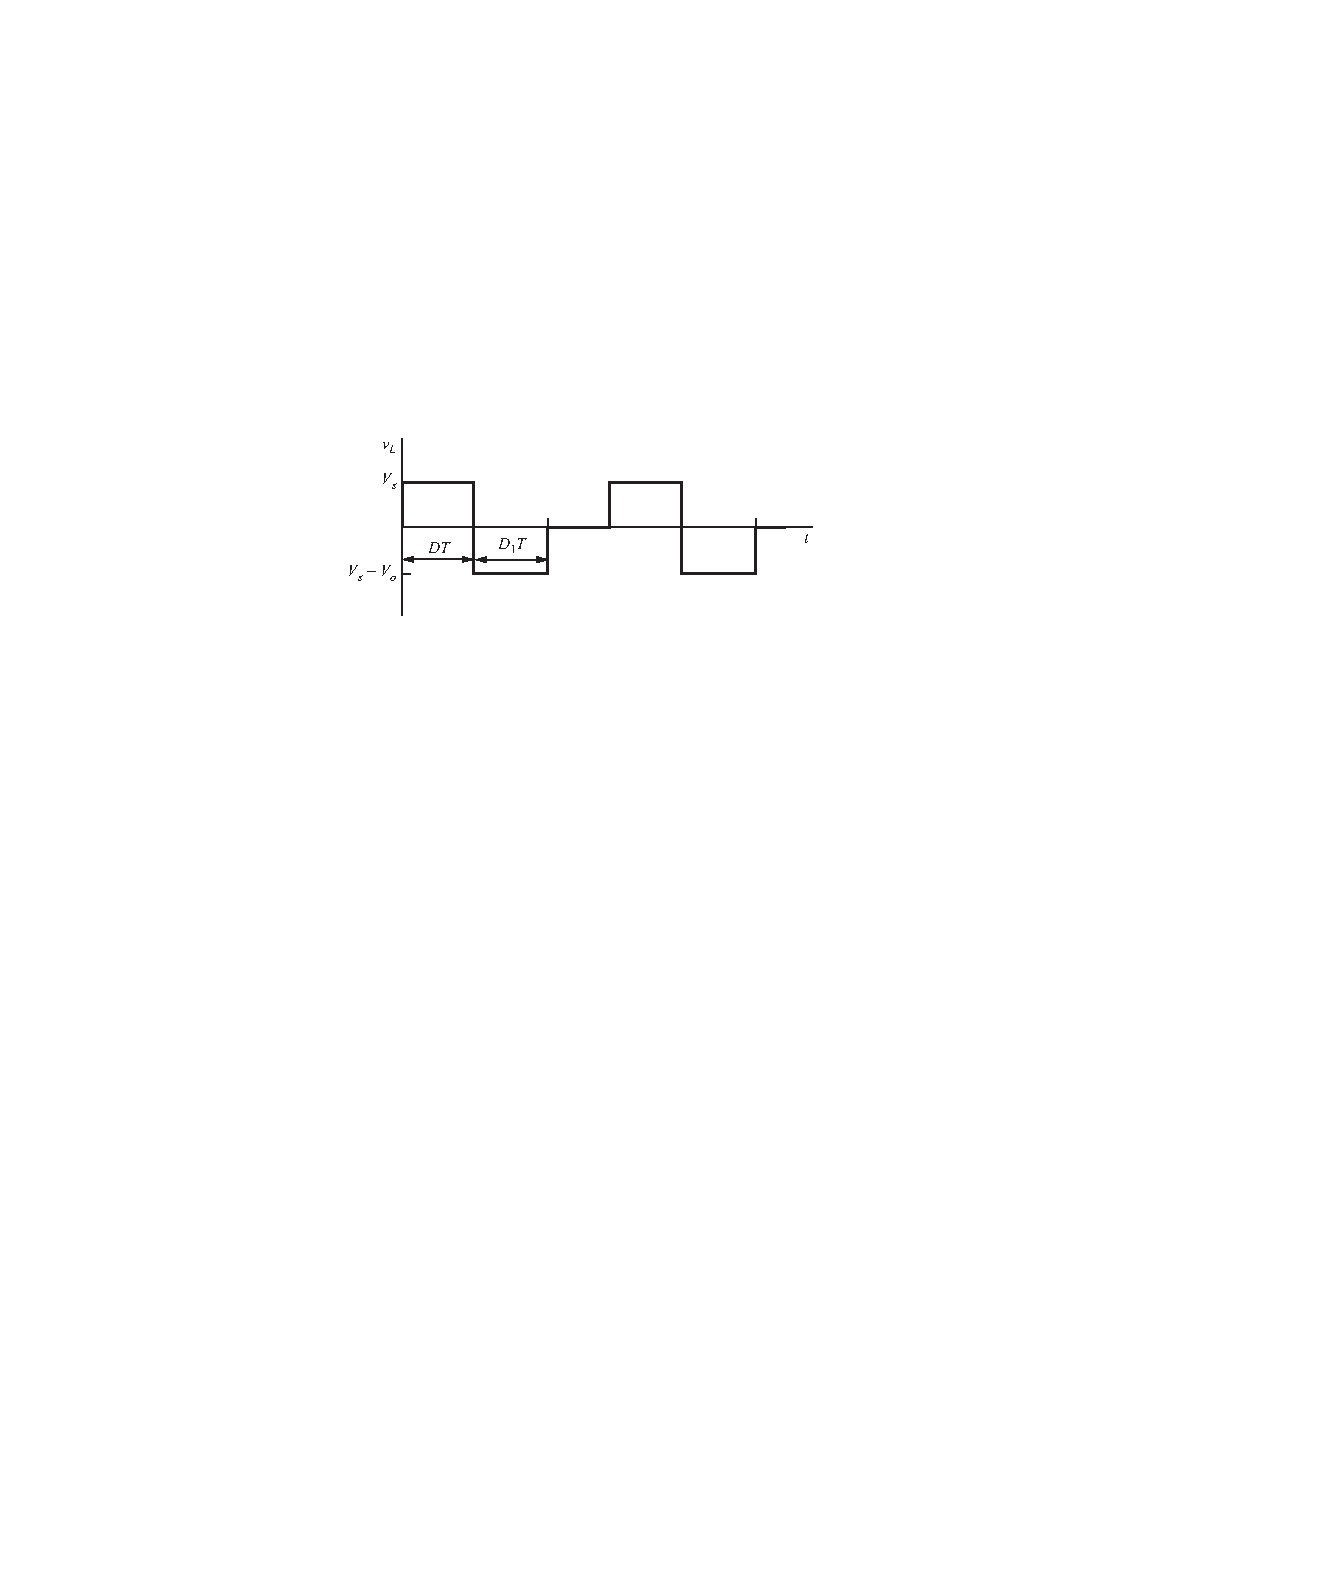
\includegraphics[width=0.38\textwidth]{Imágenes/Convertidor elevador/Modo de conducción discontinua/Tensión del inductor.pdf}}    
    \hspace{10mm}
    \subfloat[Corriente por el inductor.]{\includegraphics[width=0.38\textwidth]{Imágenes/Convertidor elevador/Modo de conducción discontinua/Corriente del inductor.pdf}}
    \hspace{10mm}
    \subfloat[Corriente por el diodo]{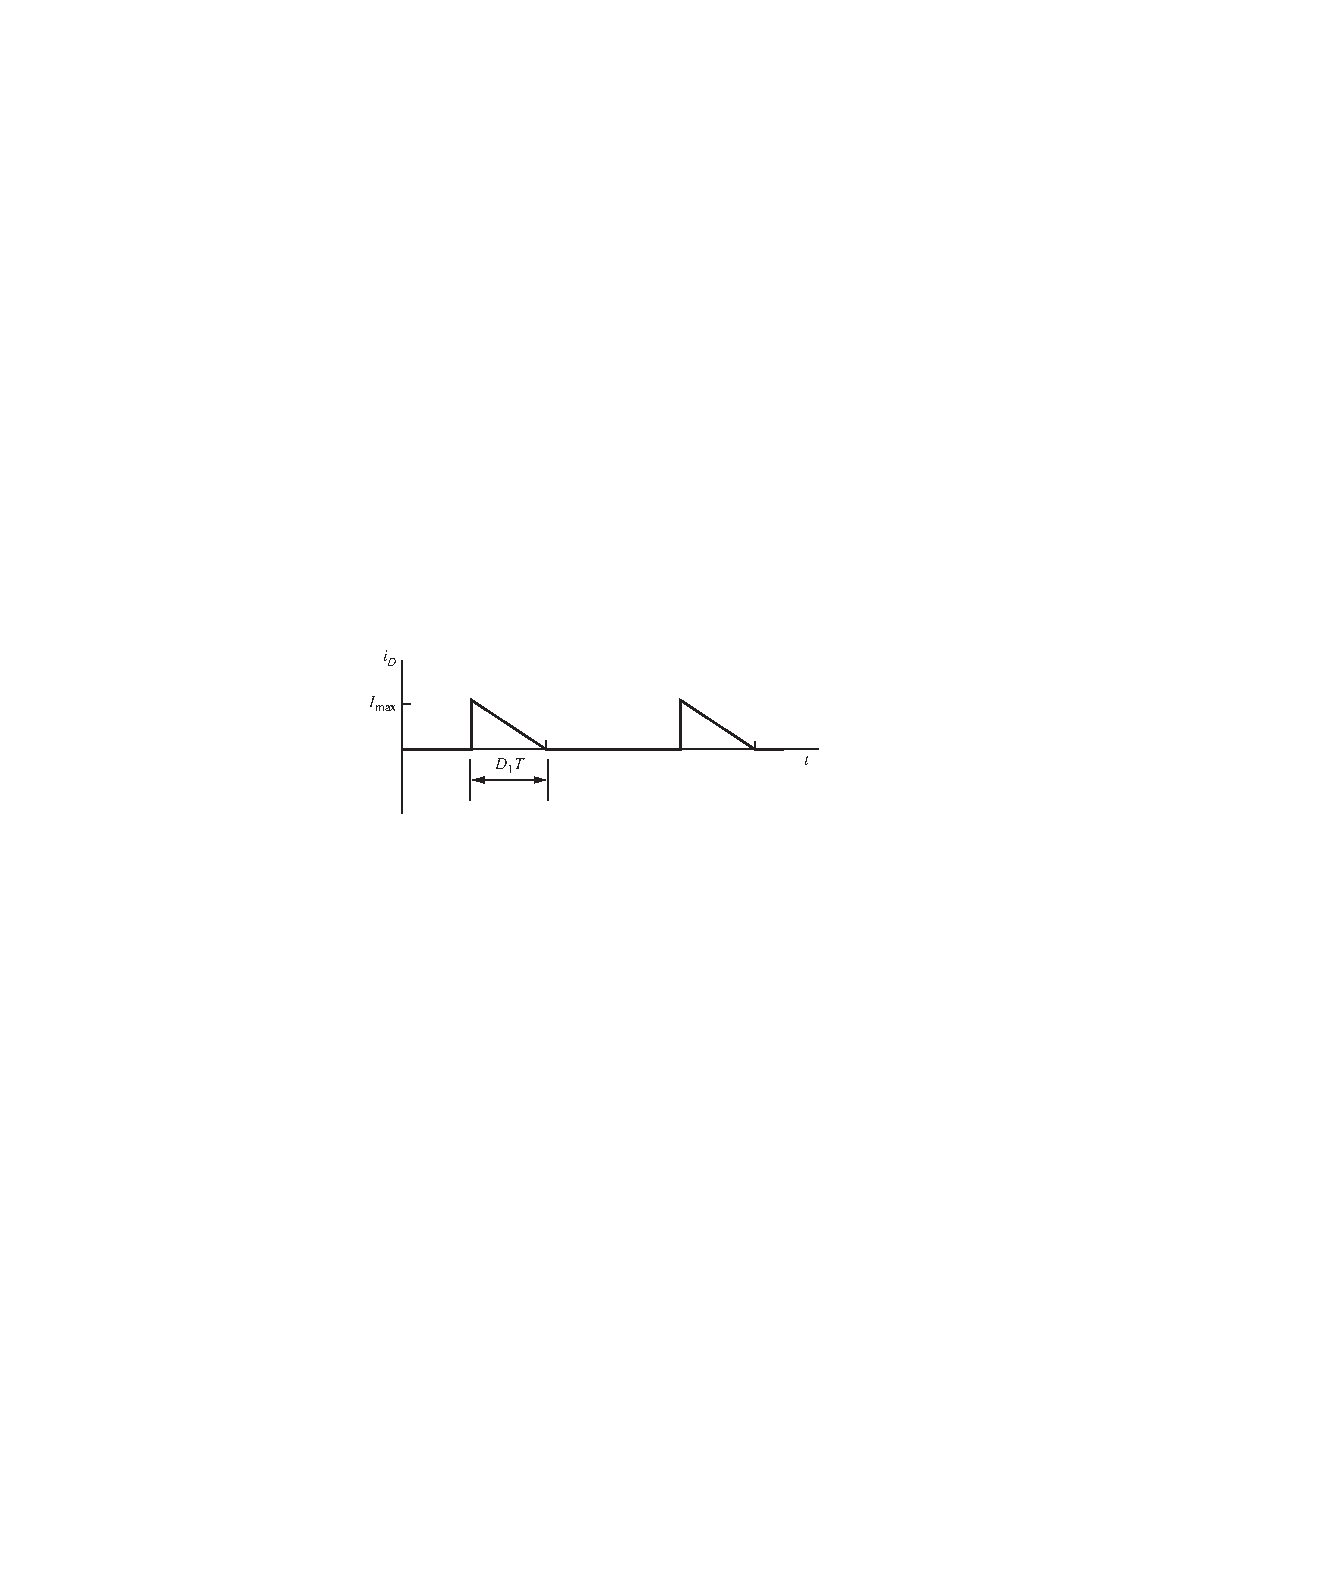
\includegraphics[width=0.38\textwidth]{Imágenes/Convertidor elevador/Modo de conducción discontinua/Corriente del diodo.pdf}}
    \caption{Formas de onda de un convertidor elevador en MCD.}
    \label{formas-onda-elevador-mcd}
\end{figure}

Cuando la llave está cerrada, la tensión a lo largo del inductor es $V_s$. Y cuando está abierta y la corriente por el inductor es positiva, su tensión es $V_s - V_o$. La corriente del inductor disminuye hasta que llega a cero, y el diodo previene que esta se haga negativa. Cuando la llave está abierta y el diodo polarizado en inversa, la corriente del inductor es nula. La tensión media que cae en el inductor es:

\begin{equation*}
    V_s D T + (V_s - V_o) D_1 T = 0
\end{equation*}

Lo que resulta en:

\begin{equation}
    V_o = V_s \left(\frac{D+D_1}{D_1}\right)
    \label{tension-salida-mcd-temp}
\end{equation}

La corriente media en el diodo (Figura \ref{formas-onda-elevador-mcd}c) es: 

\begin{equation}
    I_D = \frac{1}{T} \left(\frac{1}{2} I_{max} D_1 T\right) = \frac{1}{2} I_{max} D_1
    \label{i-diodo-temp}
\end{equation}

en donde la corriente $I_{max}$ es la misma que el cambio en la corriente del inductor cuando la llave está cerrada.

\begin{equation}
    I_{max} = \Delta i_L = \frac{V_s D T}{L}
    \label{i-inductor-max}
\end{equation}

Substituyendo la Ec. \ref{i-inductor-max} en la Ec. \ref{i-diodo-temp} e igualando con la corriente de la carga,

\begin{equation}
    I_D = \frac{1}{2} \frac{V_s D T}{L} D_1 = \frac{V_o}{R}
\end{equation}

Y despejando $D_1$,

\begin{equation}
    \boxed{D_1 = \left(\frac{V_o}{V_s}\right) \left(\frac{2L}{R D T}\right)}
\end{equation}

Substituyendo esta expresión por $D_1$ en \ref{tension-salida-mcd-temp}, resulta en la siguiente ecuación cuadrática:

\begin{equation*}
    \left(\frac{V_o}{V_s}\right)^2 - \frac{V_o}{V_s} - \frac{D^2 R T}{2L} = 0
\end{equation*}

Y finalmente resolviendo para $V_o / V_s$,

\begin{equation}
    \boxed{\frac{V_o}{V_s} = \frac{1}{2} \left(1 + \sqrt{1 + \frac{2 D^2 R T}{L}}\right)}
\end{equation}

La situación límite entre corriente continua y discontinua ocurre cuando $D_1 = 1 -D$. Otra condición límite es cuando $I_{min}$ es menor o igual a cero.

El modo de operación del convertidor depende de la combinación de los parámetros del circuito, incluyendo el ciclo de trabajo. Si este ciclo de trabajo $D$ es variado, el convertidor puede entrar y salir del modo de conducción discontinua. La Figura \ref{modo-conduccion-elevador} muestra la tensión de salida para un convertidor elevador respecto del ciclo de trabajo.

\begin{figure}[hbt!]
    \centering
    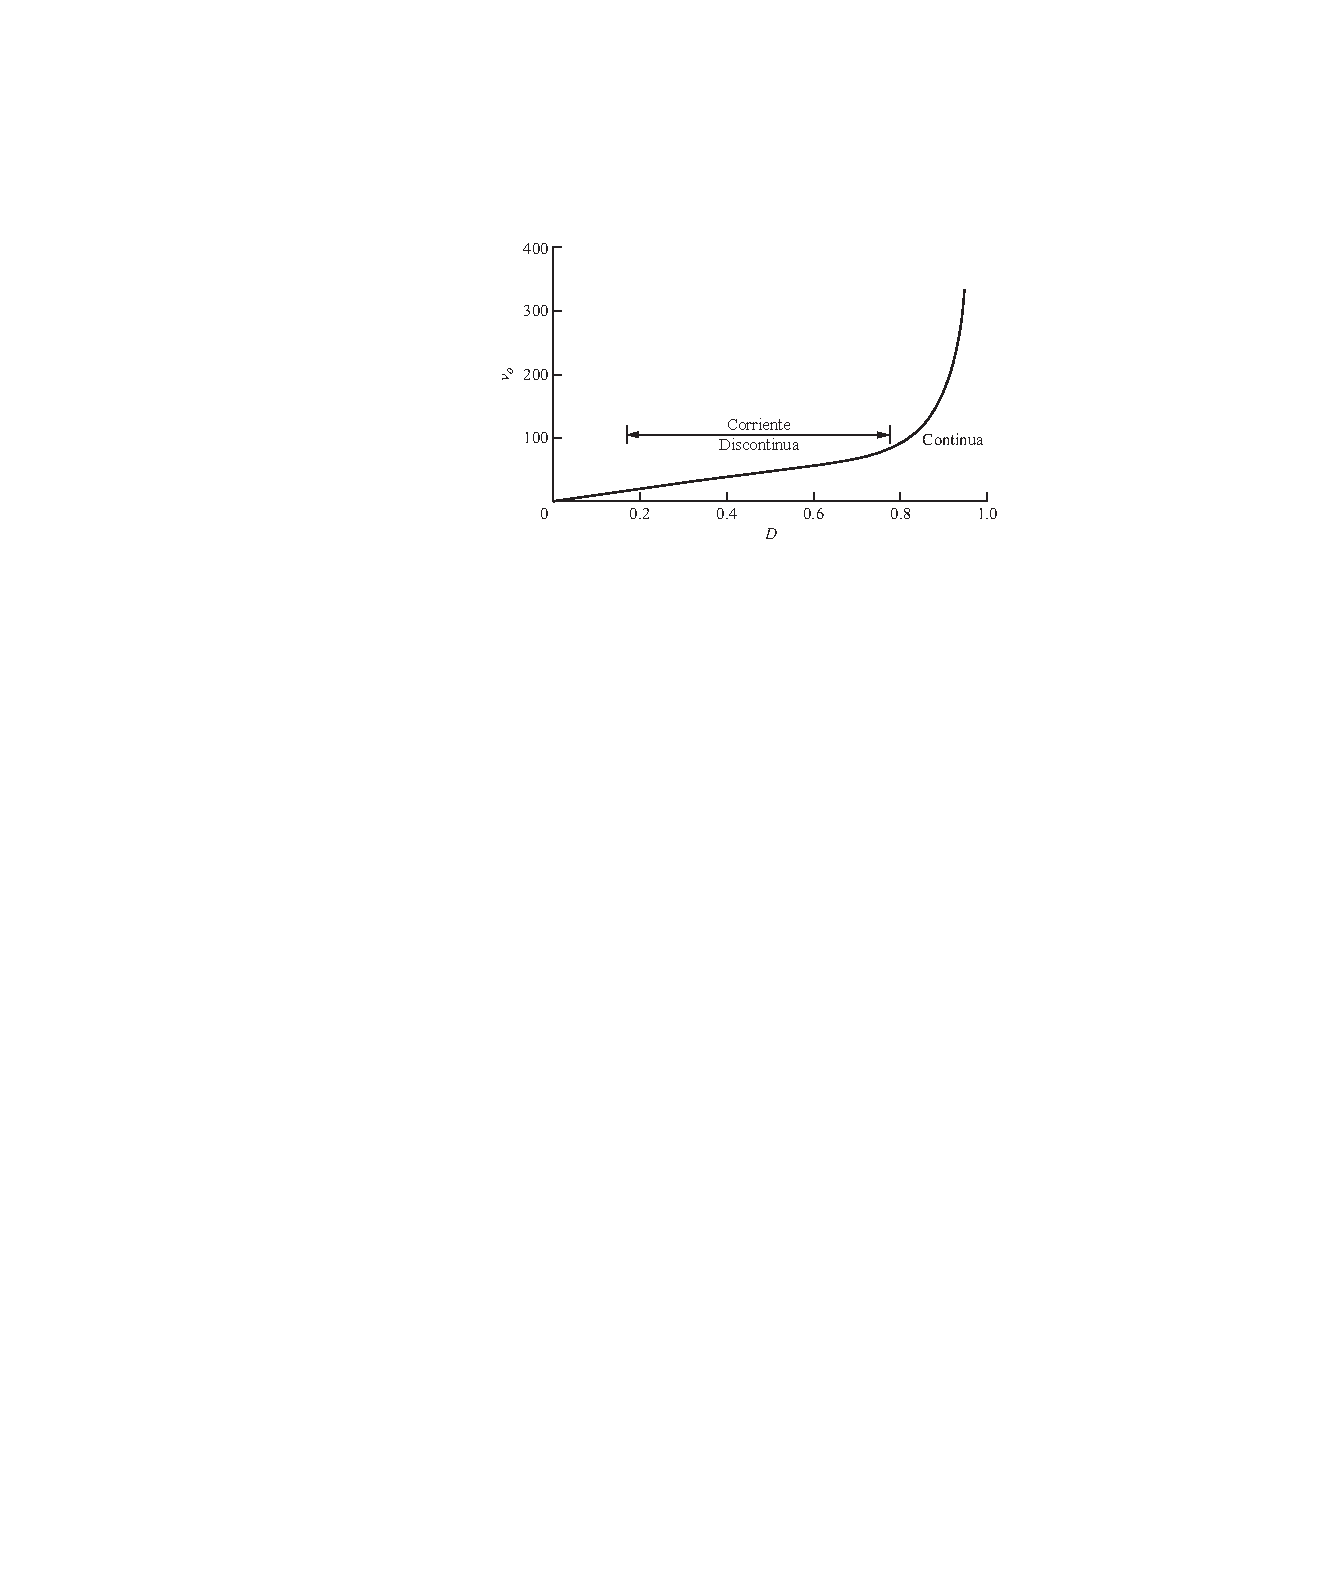
\includegraphics[width=0.55\columnwidth]{Imágenes/Convertidor elevador/Modo de conducción discontinua/Tension de salida respecto del ciclo de trabajo.pdf}
    \caption{Tensión de salida de un circuito elevador.}
    \label{modo-conduccion-elevador}
\end{figure}

\subsection{Convertidor elevador bidireccional en corriente}
\label{presentacion-convertidor}

Este tipo de convertidor es más versátil que la topología elevadora convencional, dado que tiene la capacidad de transferir energía en ambos sentidos, de la entrada a la salida y viceversa, efectuando únicamente un cambio en el sentido de la corriente.

Un convertidor elevador bidireccional en corriente se construye sustituyendo el diodo que se encuentra en la topología elevadora convencional por un transistor controlado que permita el flujo de corriente en ambas direcciones. En particular, durante el proceso de fabricación de un transistor \mbox{MOSFET} se forma una juntura p-n entre los terminales de \emph{drain} y \emph{source}, permitiendo que la corriente pueda establecerse en la dirección opuesta \emph{source-drain}. De esta forma se obtiene la bidireccionalidad de corriente a través de la llave. La topología resultante se muestra en la Figura \ref{convertidor-bidireccional}.

\begin{figure}[hbt!]
    \centering
    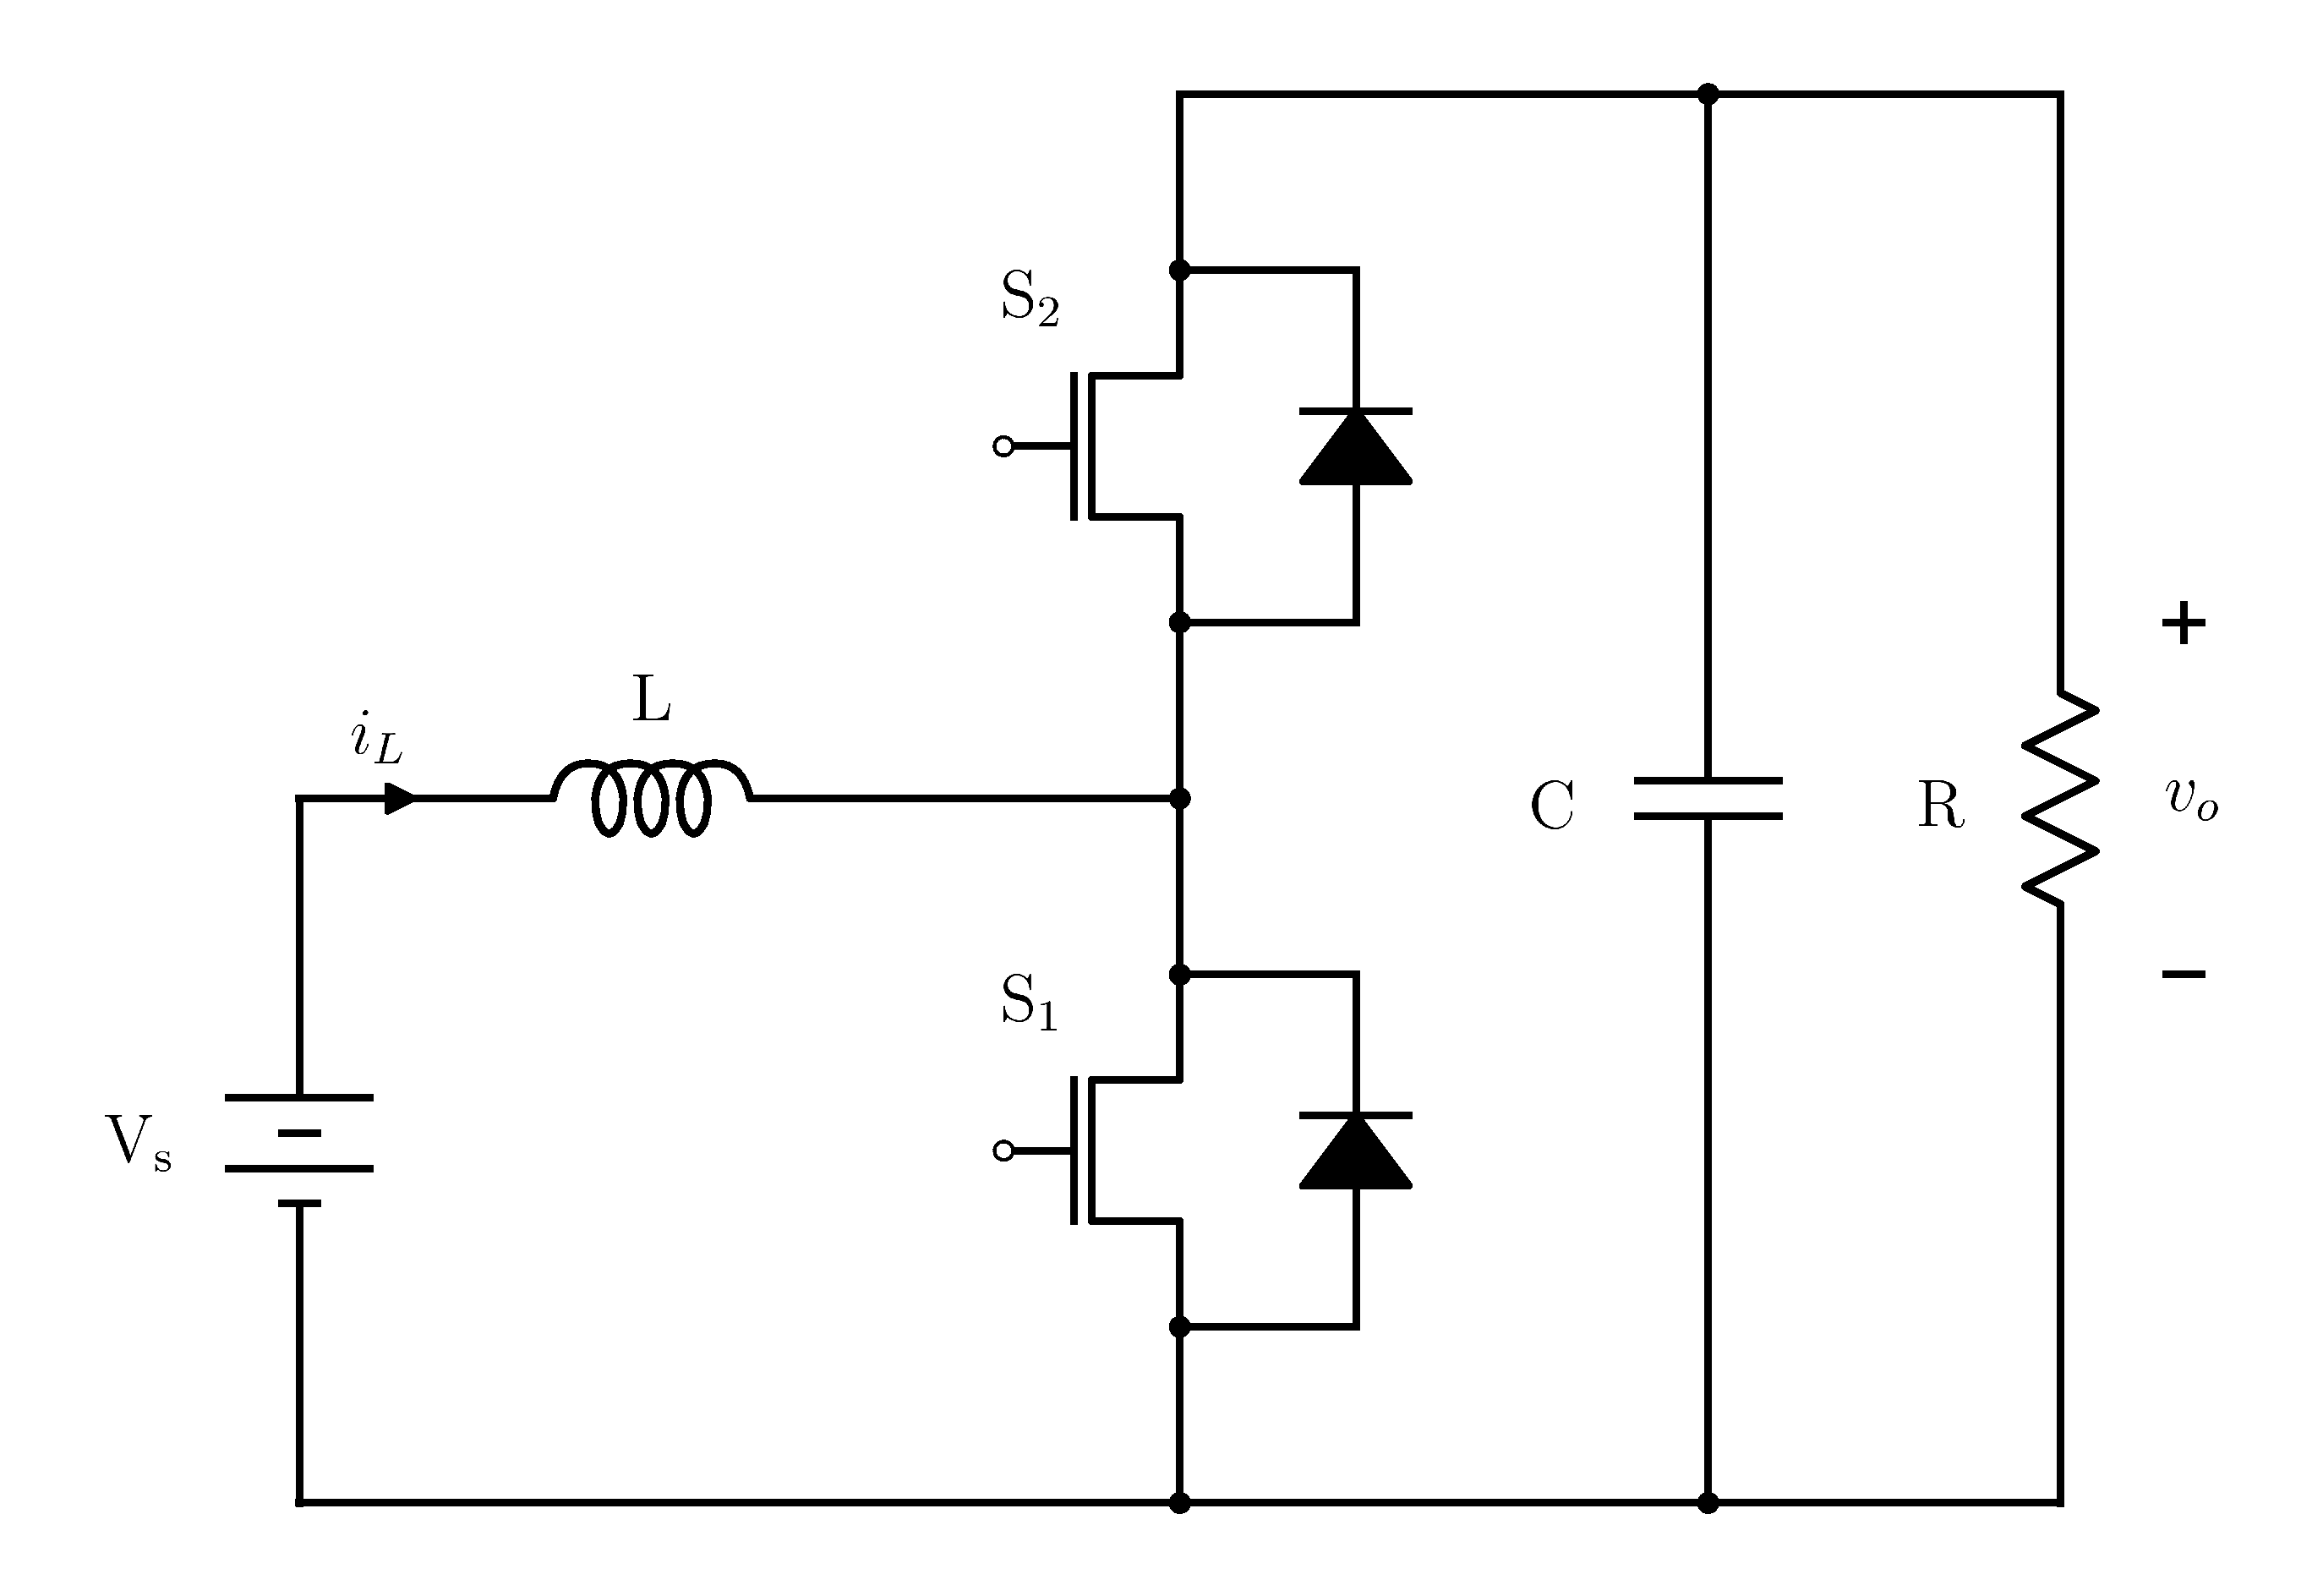
\includegraphics[width=0.40\columnwidth]{Imágenes/Diseño del control/Convertidor bidireccional de corriente.pdf}
    \caption{Convertidor elevador bidireccional en corriente.}
    \label{convertidor-bidireccional}
  \end{figure} 

Un ejemplo práctico de la aplicación de convertidores bidireccionales que facilita la comprensión de su utilidad se encuentra en el sistema de distribución de un vehículo híbrido. El vehículo tiene esencialmente 2 modos de operación:

\begin{itemize}
    \item \textbf{Modo marcha}: Para ponerse en marcha, el vehículo toma energía del banco de supercapacitores durante la aceleración y de las baterías de litio una vez estabilizada su velocidad. Durante este proceso, el convertidor transfiere energía desde los módulos de almacenamiento hacia el vehículo.
    \item \textbf{Modo regenerativo}: Una vez que el vehículo está en marcha, existe una regeneración de energía que es devuelta a los módulos de almacenamiento por parte del sistema electromecánico. Durante este proceso, el convertidor transfiere energía desde el vehículo hacia los módulos de almacenamiento.
\end{itemize}

El ejemplo anterior pone de manifiesto la gran versatilidad que se obtiene al modificar la topología elevadora clásica para lograr bidireccionalidad en el flujo de energía.

\begin{figure}[hbt!]
    \centering
    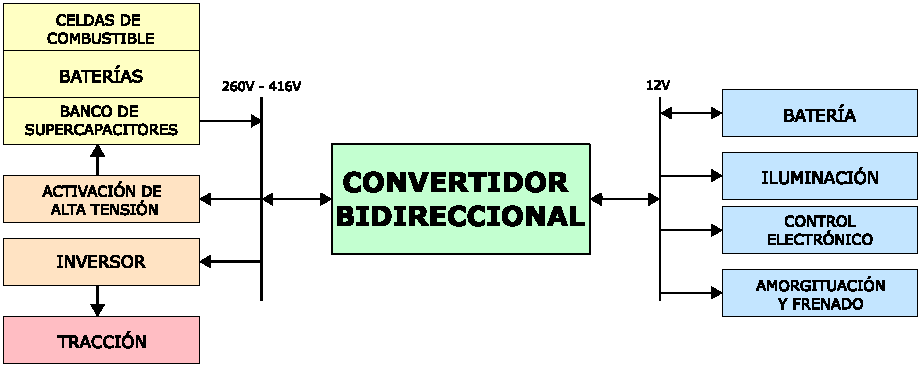
\includegraphics[width=0.75\columnwidth]{Imágenes/Convertidor elevador/Sistema eléctrico de un vehículo híbrido.pdf}
    \caption{Sistema eléctrico de un vehiculo híbrido.}
    \label{sistema-electrico-hev}
\end{figure} 

En este trabajo se utiliza un convertidor CC-CC bidireccional en corriente construido en el instituto (Figura \ref{convertidor-leici}) \cite{caravelli}. Este convertidor cuenta con una etapa de instrumentación que permite la medición de las corrientes y tensiones entrantes y salientes. En la Tablas 2.1a y 2.1b se muestran sus especificaciones técnicas.

\begin{figure}[hbt!]
    \centering
    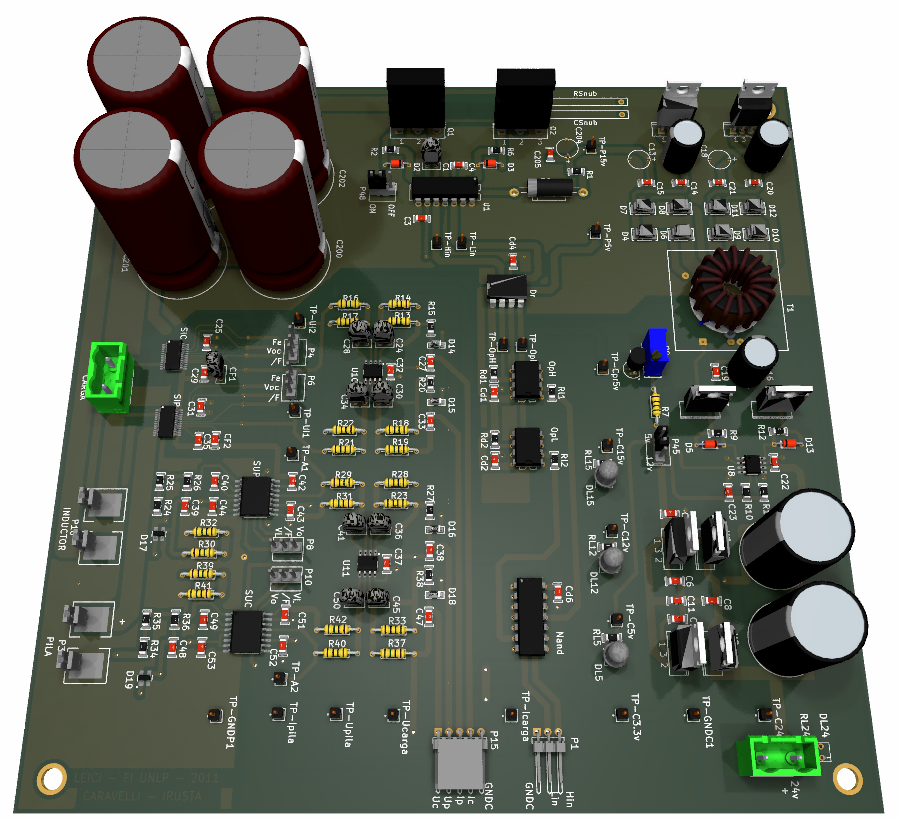
\includegraphics[width=0.52\columnwidth]{Imágenes/Convertidor elevador/Vista 3D del PCB del convertidor DC-DC.png}
    \caption{Vista 3D del convertidor DC-DC utilizado en el proyecto.}
    \label{convertidor-leici}
\end{figure} 

\begin{figure}
\begingroup
\renewcommand{\figurename}{Tabla}
\setcounter{figure}{0}
\centering
\subfloat[Parámetros reelevantes]{
    \begin{tabular}{lll}
        \label{parametros-convertidor}
        Especificación                     & Valor & Unidad \\
        \hline
        \\
        Potencia máxima                    & 300   & W      \\
        \makecell[l]{Tensión continua \\ en la salida}      & 60    & V      \\
        \makecell[l]{Tensión nominal  \\ en la entrada}      & 20    & A      \\
        \makecell[l]{Corriente nominal \\ en la entrada}    & 15    & A      \\
        \makecell[l]{Rizado pico a pico \\ de la corriente} & 3.33  & A      \\
        \makecell[l]{Frecuencia de \\ conmutación}          & 20    & kHz     \\
        Inductancia                        & 200   & H      \\
        \makecell[l]{Corriente máxima \\ por el inductor}   & 16.67 & A      \\
        Capacitancia                       & 2200  & \SI{}{\micro\farad}
    \end{tabular}
}
\subfloat[Componentes de la etapa de potencia]{
    \begin{tabular}{lll}
        \label{componentes-convertidor}
        Componente          & Denominación    & Comentarios                                                    \\
        \hline\\
        \makecell[l]{Núcleo del \\ inductor} & ETD-5922 CF-138 & \makecell[l]{Permeabilidad relativa \\ $\mathrm{\mu_r}$ de 2500}                           \\
        Capacitor           & TREC            & \makecell[l]{Tensión máxima de \\ trabajo de \SI{100}{V}}                              \\
        Interruptores       & IRFP-250        & \makecell[l]{MOSFET con corriente \\ máxima de drenador de \SI{30}{A}}                \\
        Drivers             & IR2110          & \makecell[l]{Tiempo de encendido \\ y apagado de \SI{120}{\nano\second} y \SI{94}{\nano\second} \\ respectivamente} \\
        \makecell[l]{Diodo de \\ bootstrap}  & MUR 460         & \makecell[l]{Capacitancia de \SI{1}{\micro\farad} \\ con resistencia de \SI{2.2}{\ohm}}               
    \end{tabular}
} 
\caption{Tablas con especificaciones del convertidor CC-CC.}
\endgroup
\end{figure}    

\section{Resumen}

En este capítulo se ha analizado el funcionamiento de la topología de convertidor CC-CC elevador bajo distintas condiciones de conducción, y realizando una leve modificación en su estructura, se logra un tipo de convertidor CC-CC bidireccional en corriente. Finalmente, se presenta específicamente al convertidor utilizado en este proyecto.

\newpage

\chapter{Field-programmable gate arrays}
\label{cap-fpga}

\section{Introducción}

Las \emph{field-programmable gate arrays} (FPGAs) son dispositivos basados en una matriz de bloques lógicos configurables (CLBs) conectados vía interconexiones programables.
Las FPGAs pueden ser reprogramadas para cualquier aplicación o funcionalidad requerida mientras se encuentre dentro de las limitaciones de la placa. Esta característica las diferencia de las \emph{application specific integrated circuits} (ASICs), las cuales son diseñadas específicamente para ciertas tareas.

En este capítulo se explican distintas características de este tipo de dispositivos, así como los entornos de desarrollos que alrededor de ellos. Primero, se detalla su arquitectura y los bloques elementales que lo conforman, para después informar al lector de los particulares lenguajes de programación utilizados para su programación y los paradigmas en los que se basan. Por último, se enumeran distintas herramientas de software que se emplean para su programación. 

\section{Arquitectura}

Los FPGAs modernos poseen grandes recursos de bloques lógicos y de RAM para implementar calculos complejos, y también periféricos como conversores analógicos-digitales (ADCs) y conversores digitales-analógicos (DACs). La arquitectura básica de un FPGA puede observarse en la Figura \ref{fpga}, la cual consiste de un arreglo de CLBs, pads de entrada/salida (I/O), y canales de enrutamiento.

\begin{figure}[hbt!]
    \centering
    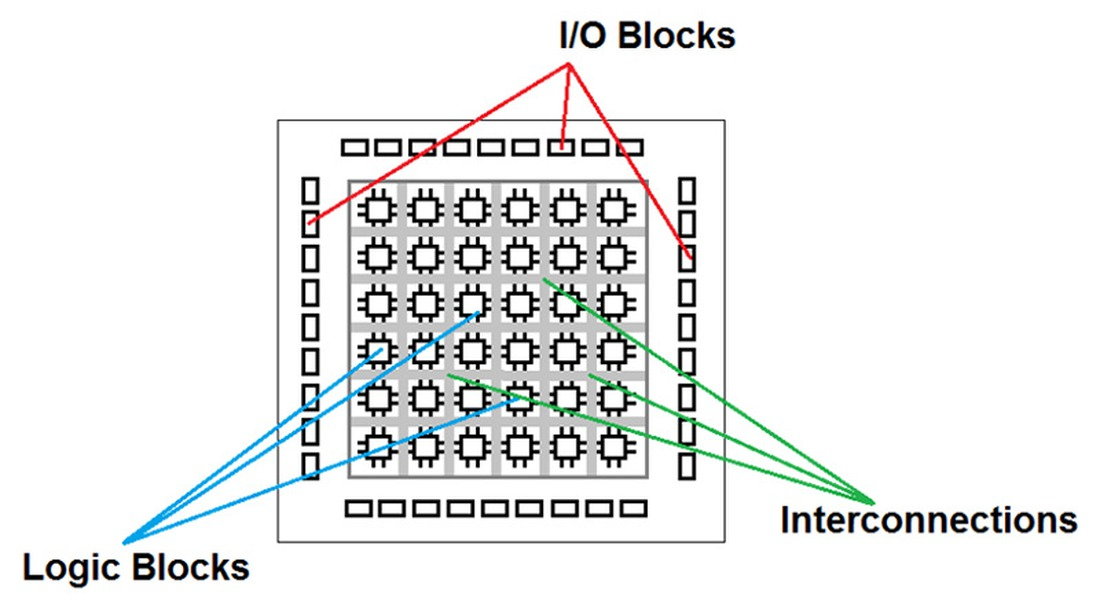
\includegraphics[width=0.45\columnwidth]{Imágenes/Arquitectura de un FPGA.png}
    \caption{Arquitectura básica de un FPGA.}
    \label{fpga}
\end{figure} 

\subsection{Bloques lógicos}

Generalmente, los bloques lógicos de un FPGA consisten de algunas celdas lógicas (llamadas ALM, LE, slices, etc.). Típicamente, estas celdas consisten en una \emph{lookup table} (LUT) con 4 entradas, un \emph{full adder} (FA), y un flip-flop tipo D (DFF). Estos bloques lógicos poseen distintos modos los cuales le otorgan flexibilidad a la hora del uso de sus componentes, y por lo tanto amplía sus funcionalidades. Por ejemplo, en la Figura \ref{clb} puede observarse una celda lógica, perteneciente a un CLB. En ella, hay LUTs de 3 entradas, las cuales mediante un multiplexor, pueden ser combinadas para conseguir una LUT de 4 entradas. Además, la salida de estas celdas lógicas puede ser sincrónicas o asincrónicas, decisión dictada por otro multiplexor.

\begin{figure}[hbt!]
    \centering
    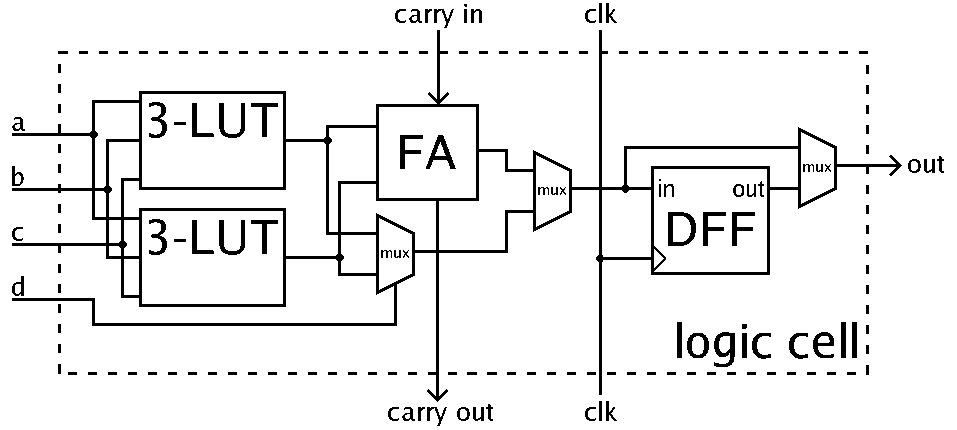
\includegraphics[width=0.65\columnwidth]{Imágenes/Celda lógica de CLB.png}
    \caption{Ilustración simplificada de una celda lógica.}
    \label{clb}
\end{figure} 

\subsection{Integración}
\label{subseccion-nexys-3}

Actualmente, estos bloques lógicos e interconexiones de los FPGAs tradicionales son combinados con microprocesadores embebidos y otros bloques de funcionalidad de alto nivel (multiplicadores, bloques de procesamiento de señales, memorias embebidas, etc.) para formar un \emph{system on chip} (SoC). Un ejemplo de este nuevo enfoque de las FPGAs puede verse en la Figura \ref{spartan6}.   

\begin{wrapfigure}{l}{0.5\textwidth}
    \vspace{-0pt}
    \begin{center}
      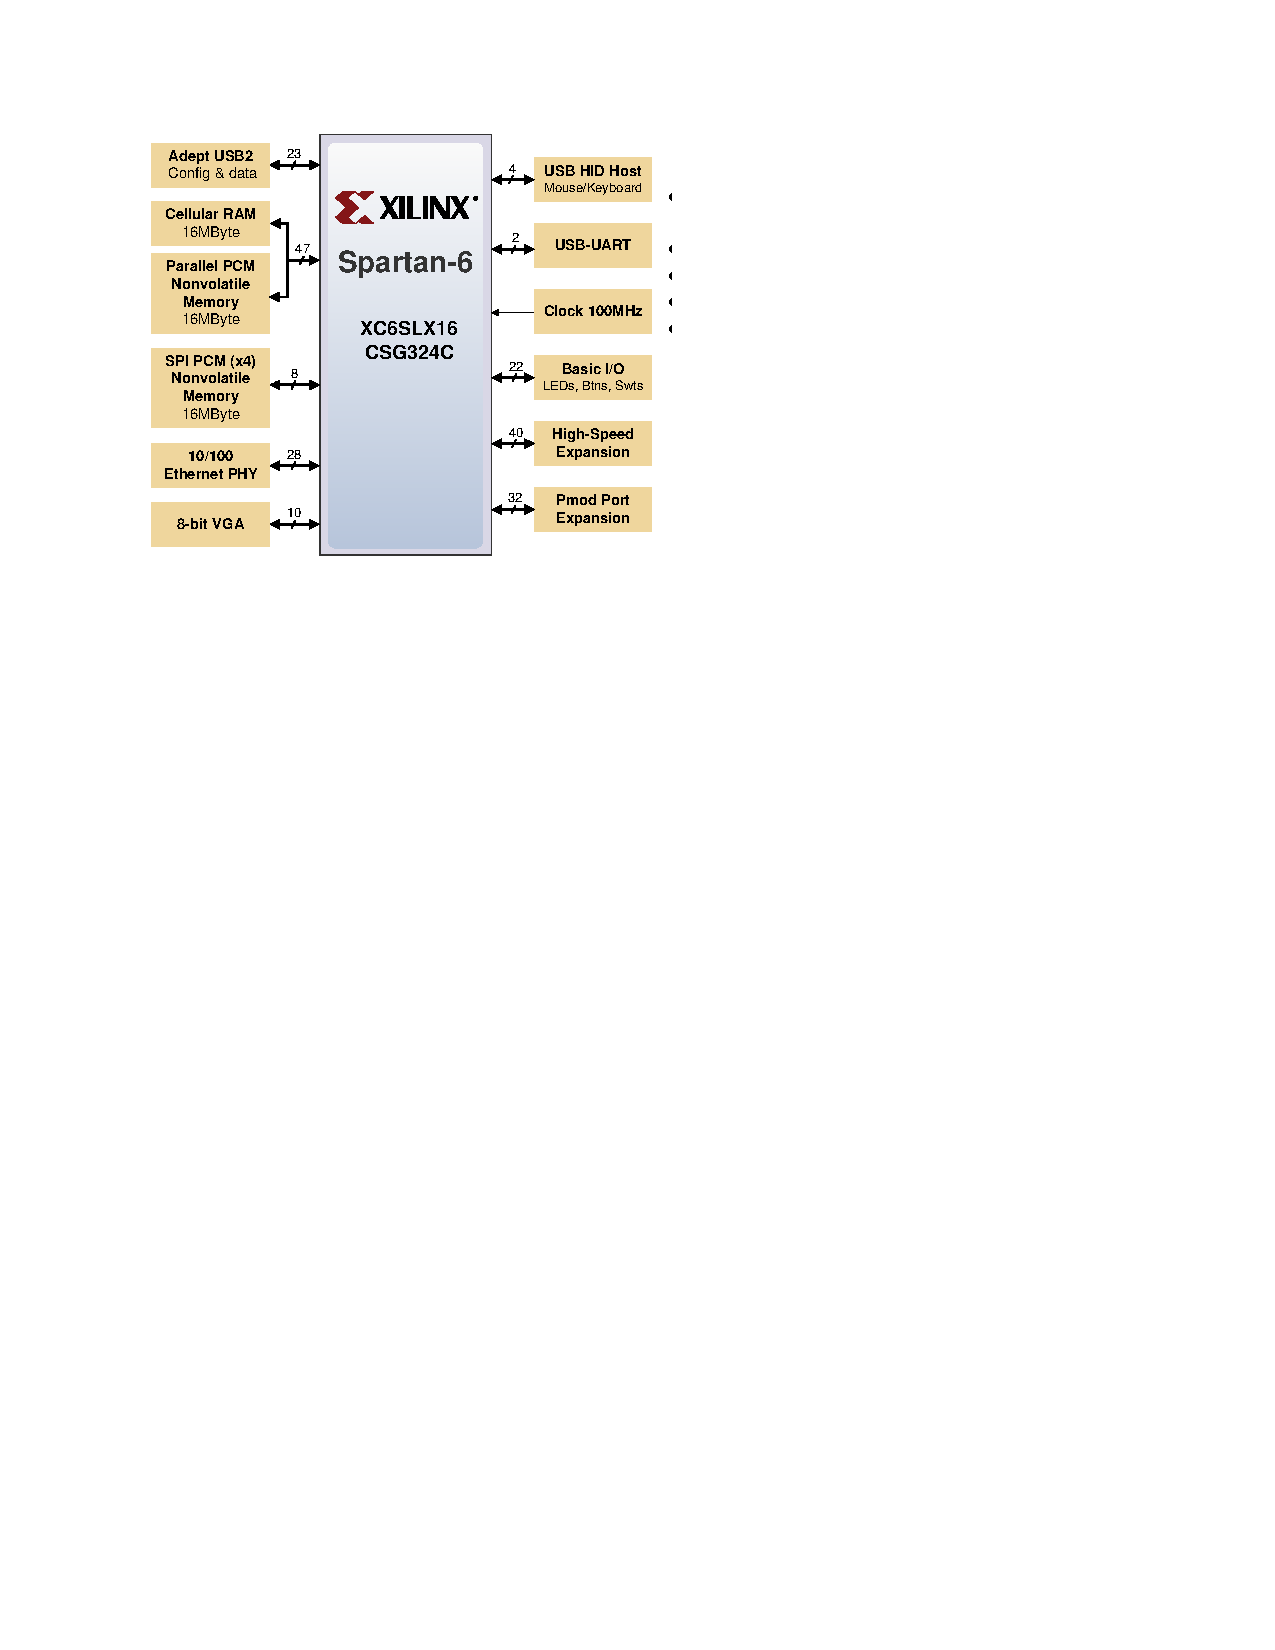
\includegraphics[width=0.41\textwidth]{Imágenes/SoC del Nexys 3.pdf}
    \end{center}
    \caption{Spartan-6 de Xilinx en la placa de desarrollo Nexys 3.}
    \label{spartan6}
  \end{wrapfigure}

Aqui, se puede observar un diagrama de conexionado del FPGA Spartan-6, utilizado en la placa de desarrollo Nexys 3. Además de poseer varios tipos de conexiones, el Spartan-6 posee 2278 \mbox{\emph{slices}} o celdas lógicas, en las cuáles cada una posee cuatro LUTs de 6 entradas y ocho flip-flops. Además, posee 576 kB de RAM, 32 slices enfocados a DSP, y velocidades de reloj de más de \SI{500}{\mega\hertz}. 

A su vez, la placa de desarrollo amplía aún más sus funcionalidades, brindando una colección mejorada de periféricos, como por ejemplo un puerto USB-UART, 16MB de RAM, y 10/100 Ethernet PHY, entre otros \cite{nexys3}.

Esto deja en claro que el objetivo de las FPGAs es proveer flexibilidad a la hora de su uso, brindando una gran variedad de herramientas para cualquier aplicación. Por eso mismo es que este tipo de circuitos es ideal para desarrollar prototipos en las fases iniciales de un proyecto.

\section{Lenguajes de descripción de hardware}

Los lenguajes de descripción de hardware (HDL) son lenguajes de programación utilizados para describir la estructura y comportamiento de circuitos lógicos digitales. Este tipo de lenguajes permite la síntesis de una descripción por HDL a una \emph{netlist} (interconexión de componentes electrónicos físicos descriptos), la cual puede ser implementada para finalmente crear un circuito integrado.

Los HDLs forman una parte íntegra de la automatización de diseño electrónico (EDA, del inglés \mbox{\emph{electronic design automation}}), especialmente para circuitos complejos, y son los lenguajes utilizados en la programación de los FPGAs. Los dos lenguajes más utilizados son Verilog, y VHDL.

\subsection{Verilog}

En Verilog, el diseño consiste de una jerarquía de módulos. Estos módulos son definidos con conjuntos de puertos de entrada, salida y bidireccionales. Internamente, un módulo contiene una lista de cables y registros. Las sentencias concurrentes y secuenciales definen el comportamiento del módulo, describiendo las relaciones entre los puertos, cables, y registros. Las sentencias secuenciales son colocadas dentro de un boque \texttt{begin}/\texttt{end} y ejecutadas en orden secuencial, pero todas las sentencias concurrentes y todos los bloques \texttt{begin}/\texttt{end} son ejecutados en paralelo en el diseño. Un módulo puede contener una o más instancias de otro módulo para definir un subcomportamiento.

Un subconjunto de sentencias en el lenguaje es sintetizable. Si los módulos en un diseño contienen sólo sentencias sintetizables, puede ser sintetizado en una \emph{netlist} que describe los componentes básicos y los conectores que deben implementarse en hardware. La \emph{netlist} o lista de nodos puede ser entonces convertido en un \emph{bitstream} para programar el FPGA.

\subsection{VHDL}

VHDL (acrónimo de \emph{Very High Speed Hardware Description Language} en inglés) es un HDL que hereda muchos conceptos de lenguajes de programación a alto nivel (por ejemplo C o PASCAL). Una característica importante heredada es el concepto de tipos de datos. Por ejemplo, los tipos de datos \emph{bit}, \emph{boolean}, \emph{integer}, etc. ya se encuentran incorporados, pero existe la posibilidad de definir nuevos tipos, como por ejemplo matrices, registros, o punteros. Esto permite una programación a un distinto nivel de atracción.

Otra característica no menor es la del control de flujo, incorporando condicionales (\emph{if}, \emph{case}) e iteraciones (\emph{for}, \emph{while}). Además, es posible estructurar o modularizar el código, ya que se pueden agrupar partes del código en subprogramas en funciones (\emph{function}) o procedimientos (\emph{procedures}), e incluye la posibilidad de desarrollar y utiliza bibliotecas de diseño.

Aunque varias características son heredadas de otros lenguajes de programación, VHDL es un HDL en sí, y por lo tanto es necesario explicar sus conceptos específicos para modelado de hardware.

\subsubsection{Modelo de estructura}
\label{vhdl-estruct}

Cualquier sistema electrónico puede dividirse en subsistemas más pequeños hasta llegar a su nivel primitivo (es decir, al nivel de puertas lógicas). Por eso mismo VHDL incorpora el concepto de estructura. Esta característica nos permite realizar el modelo de un sistema digital cualquier a partir de la referencia a las distintas partes que lo forman, especificando la conexión entre éstas. Cada una de las partes, a su vez, pueden estar modeladas de forma estructural a partir de sus componentes, o bien estar descritas de forma funciona, utilizando los conceptos heredados de los lenguajes de programación de alto nivel. En el nivel más alto de jerarquía se encuentran los modelos funcionales, a partir de los cuales se construye el sistema completo.

\begin{wrapfigure}{r}{0.45\textwidth}
  \vspace{-20pt}
  \begin{center}
    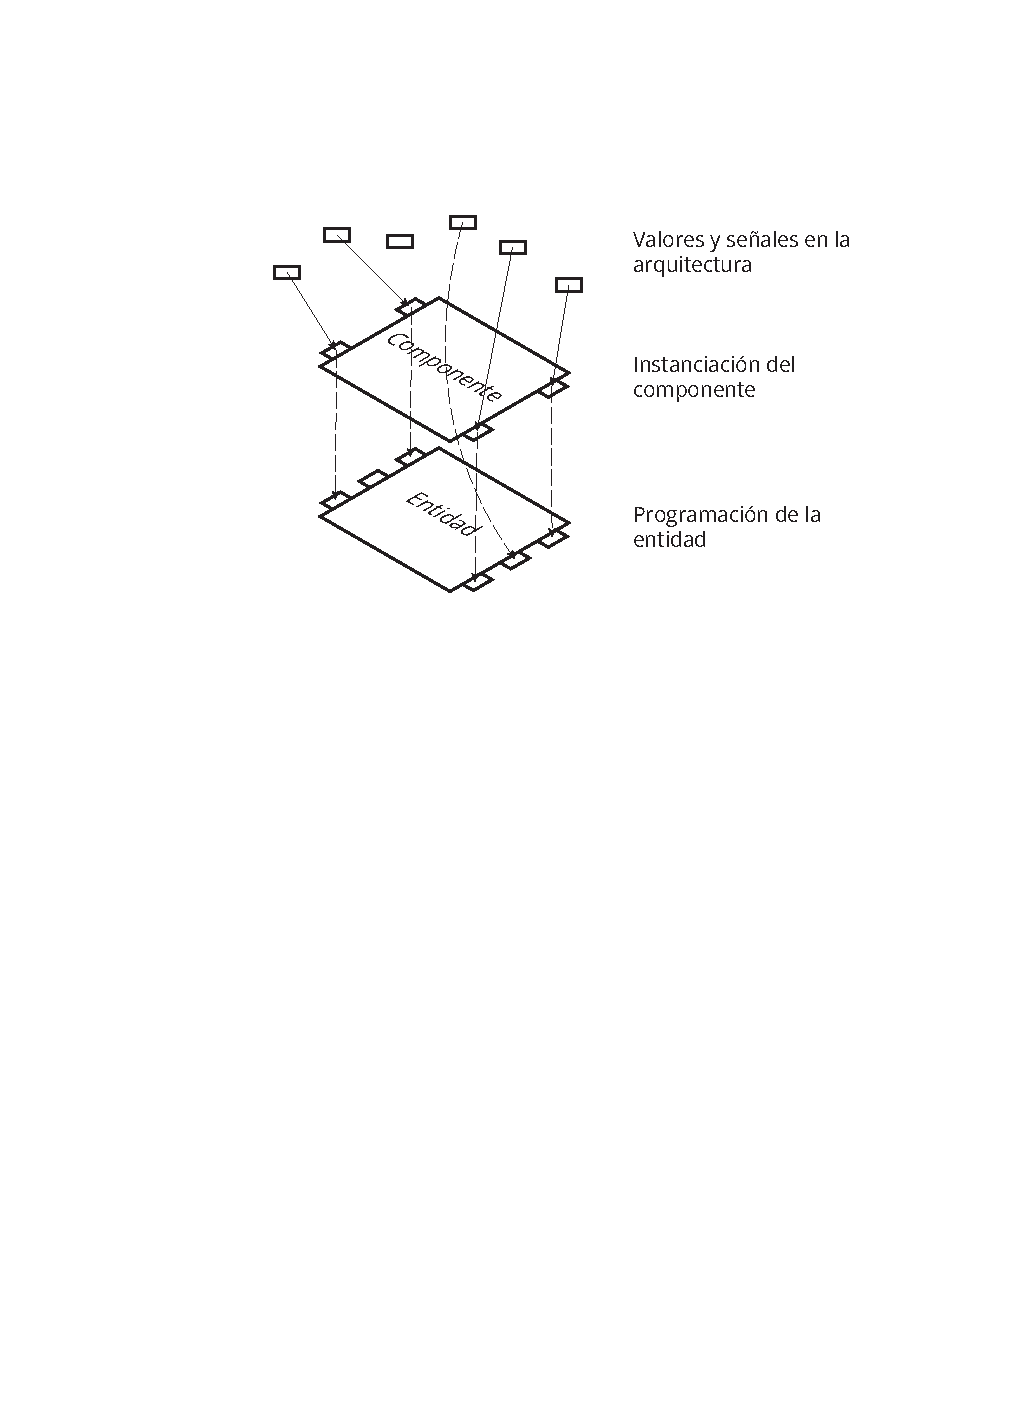
\includegraphics[width=0.41\textwidth]{Imágenes/Asociación entidad-componente.pdf}
  \end{center}
  \caption{Asociación entidad-componente-arquitectura de un modelo.}
  \label{entidad-componente}
\end{wrapfigure}

En la descripción de un dispositivo en VHDL, el diseñador debe definir dos elementos principales: la interfaz del dispositivo con el exterior (\emph{entity}) y la descripción de la funcionalidad que realiza el dispositivo \mbox{(\emph{architecture}}). La interfaz de un dispositivo tiene por objeto definir qué señales del dispositivo son visibles o accesibles desde el exterior, llamados puertos (\emph{ports}) del dispositivo. En la arquitectura se definirá la funcionalidad que implementa dicho dispositivo respecto de lo datos ingresantes a los puertos de entrada, para producir nuevos valores sobre los puertos de salida.

En la Figura \ref{entidad-componente} se representa gráficamente la asociación de una interfaz de un dispositivo a partir de la instanciación de un componente con los valores y señales de una arquitectura en donde es invocado.

VHDL además permite la instanciación de estos dispositivos a partir del concepto de componente (\emph{component}) y de referencia a un componente. Cualquier elemento modelado en VHDL puede ser utilizado como un componente de otro diseño, y para ello solamente es necesario hacer referencia al elemento a utilizar y conectar los puertos de su interfaz a los puntos necesarios para realizar el nuevo diseño.

El diseñador sólo debe preocuparse de las entradas y salidas de los subsistemas (es decir, su interfaz), y de la forma adecuada en que debe realizar su conexión bajo su modelo, pero no es necesario conocer cómo está descrito cada uno de los subsistemas.


\subsubsection{Modelo de concurrencia}

El hardware es por definición \emph{concurrente}\footnote{La concurrencia es la habilidad de diferentes partes de un algoritmo o programa de ser ejecutados fuera de orden o en un orden parcial, lo que permite su ejecución en paralelo.}, y en su última instancia cualquier dispositivo digital está formado de un mar de puertas lógicas, todas ellas funcionando en paralelo. El elemento básico que ofrece VHDL para modelar el paralelismo es el proceso (\emph{process}).

En general, el código que describe un proceso se ejecuta en forma secuencial, pero todos los procesos se ejecutarán en paralelo.

Estos procesos que se ejecutan concurrentemente deben poder comunicarse (sincronizarse) entre ellos. El elemento utilizado para esta vinculación es la señal (\emph{signal}). Cada proceso tiene un conjunto de señales a la que es sensible, lo que significa que el proceso se ejecuta cuando se produce un cambio o evento de dicha señal. La ejecución del proceso, el cual es un bucle infinito, puede ser suspendida con la sentencia \emph{wait}.

\subsubsection{Modelo de tiempo}

Una de las finalidades del modelado en VHDL del hardware es poder observar su comportamiento a lo largo del tiempo en una simulación o \emph{test bench}. Esto implica que las construcciones del lenguaje tendrán asociada una semántica respecto a la simulación, es decir, influirán en ésta provocando distintos eventos que sucederán a lo largo del tiempo, y a su vez, el modo en que se comportan las sentencias dependerá de los eventos que se sucedan a lo largo de la simulación.

Entonces, la simulación o \emph{test bench} de un modelo VHDL es una simulación dirigida por eventos. Esto significa que el simulador mantiene unas listas de eventos (cambios en las señales internas del modelo y también de las entradas y salidas) que se han de producir a lo largo del tiempo de simulación. Como el comportamiento del modelo es estable mientras no se produzca un evento, la tarea del simulador consiste en avanzar el tiempo de simulación hasta el siguiente evento y calcular sus consecuencias sobre la lista de eventos futuros.

Normalmente la reacción del modelo a un evento ocasionará la ejecución de otros eventos en un tiempo de simulación posterior que se añadirán a la lista. La simulación finaliza cuando se ha alcanzado el tiempo de simulación especificado por el usuario o cuando no existen más eventos.

\section{Entornos de desarrollo} 
\label{desarrollo-fpga}

\subsection{Intel Quartus Prime}

\emph{Intel Quartus Prime} es el entorno de diseño desarrollado por Intel (previamente por Altera). Permite al usuario el análisis y síntesis de diseños HDL, lo que habilita al desarrollador a compilar sus diseños, realizar análisis de tiempo, examinar diagramas RTL, simular la reacción de un modelo frente a distintos estímulos, y configurar el dispositivo a utilizar con el programador. Es importante aclarar que esto último solamente es posible con familias de FPGAs que Quartus Prime soporta, como por ejemplo la familia \emph{Cyclone}.
Quartus Prime incluye una implementación de VHDL y Verilog para descripción de hardware, edición visual de circuitos lógicos, y simulación de formas de onda vectoriales.

\subsection{Xilinx ISE}

\emph{Xilinx ISE} (Integrated Synthesis Environment) es una herramienta de software de Xilinx para la síntesis y análisis de diseños HDL, la cual está principalmente dirigida al desarrollo de las familias de productos de FPGAs de Xilinx (por ejemplo, Spartan-6).

Posee las mismas funcionalidades descritas anteriormente para \emph{Intel Quartus Prime}, pero además incluye otros componentes, como el \emph{Embedded Development Kit (EDK)}, \emph{Software Development Kit (SDK)}, y \emph{ChipScope Pro}. Por último, también incluye software que permite la simulación y \emph{test bench} del código, como \emph{ModelSim} e \emph{ISim}, los cuales son utilizados en el presente trabajo para verificar la correcta implementación de los algoritmos de control a lo largo del Capítulo \ref{implementacion-control}.

La interfaz de usuario principal del ISE es el \emph{Project Navigator}, el cual incluye la jerarquía de diseño (\emph{sources}), un editor de código (\emph{workplace}), una consola de salida (\emph{transcript}), y un árbol de procesos (\emph{processes}).

La jerarquía de diseño consiste en archivos de diseño (módulos), cuyas dependencias son interpretadas por el ISE y presentadas con una estructura de árbol. Para los diseños de chip único puede haber un módulo principal, con otros módulos incluidos en este, similar a la subrutina \texttt{main()} en programas C++.

Actualmente, Xilinx ISE fue descontinuado a favor de \emph{Vivado Design Suite}, el cual posee el mismo rol que ISE con características adicionales para el desarrollo de SoCs. Xilinx publicó la última versión en octubre de 2013 (versión 14.7) y no se prevén más actualizaciones. 


\section{Resumen}

En este capítulo fue presentada la arquitectura FPGA junto a dos de los lenguajes de programación de hardware más populares para su programación, como a su vez herramientas de su entorno de desarrollo que permiten sintetizar y compilar el código creado para tanto FPGAs de Xilinx como Altera.

En capítulos posteriores se podrán ver ciertas de estas herramientas en acción, al querer implementar el sistema de control diseñado.

\chapter{Diseño de la etapa de control}
\label{diseno-control}

\section{Introducción}

En el Capítulo \ref{convertidores-cc-cc} se realizó un análisis de cómo el comportamiento de un convertidor electrónico de potencia depende en gran medida de la frecuencia y el ciclo de trabajo de las señales de excitación aplicadas a sus llaves. Aún conociendo las condiciones de alimentación y carga para un convertidor CC-CC, el modo de operación a lazo abierto (es decir, sin realimentación de las variables de estado del sistema) no es práctico. Esto se debe a que la ausencia de una acción de control respecto del ciclo de trabajo incapacitaría corregir de forma eficiente desviaciones en los valores de salida ante perturbaciones en la fuente de energía o en la carga; o el riesgo que presenta la ausencia de control de las corrientes y tensiones del circuito, especialmente en los transitorios iniciales y una vez que el sistema es apagado.

Para corregir estos inconvenientes, en este capítulo se exploran y desarrollan alternativas para diseñar un control a lazo cerrado del convertidor empleado en este trabajo. Para tal fin es fundamental formar un modelo matemático que pueda representar su dinámica. Luego, se efectúan simplificaciones que permiten obtener una primer aproximación del, o de los, controladores a utilizar en base a los requerimientos de estabilidad y respuesta temporal. Por último, se simulan en herramientas de software como MATLAB\textsuperscript\textregistered \hspace{0.6pt} y Simulink\textsuperscript\textregistered \hspace{0.6pt} a estos controladores ante distintos tipos de perturbaciones, y a partir de los resultados se realizan ajustes sucesivos hasta obtener una estrategia de control satisfactoria.

\section{Modelo lineal del convertidor}

\subsection{Dinámica del convertidor}

En la Figura \ref{convertidor-bidireccional-diseno} se muestra nuevamente el diagrama circuital del convertidor CC-CC bidireccional en corriente, presentado en el Capítulo \ref{convertidores-cc-cc}, Sección \ref{presentacion-convertidor}. Se recuerda que este tipo de convertidor otorga versatilidad al sistema para su empleo en otras aplicaciones, aunque para este trabajo sólo es de interés el funcionamiento de manera unidireccional, es decir, la potencia transferida desde la fuente hacia la carga.

\begin{figure}[hbt!]
  \centering
  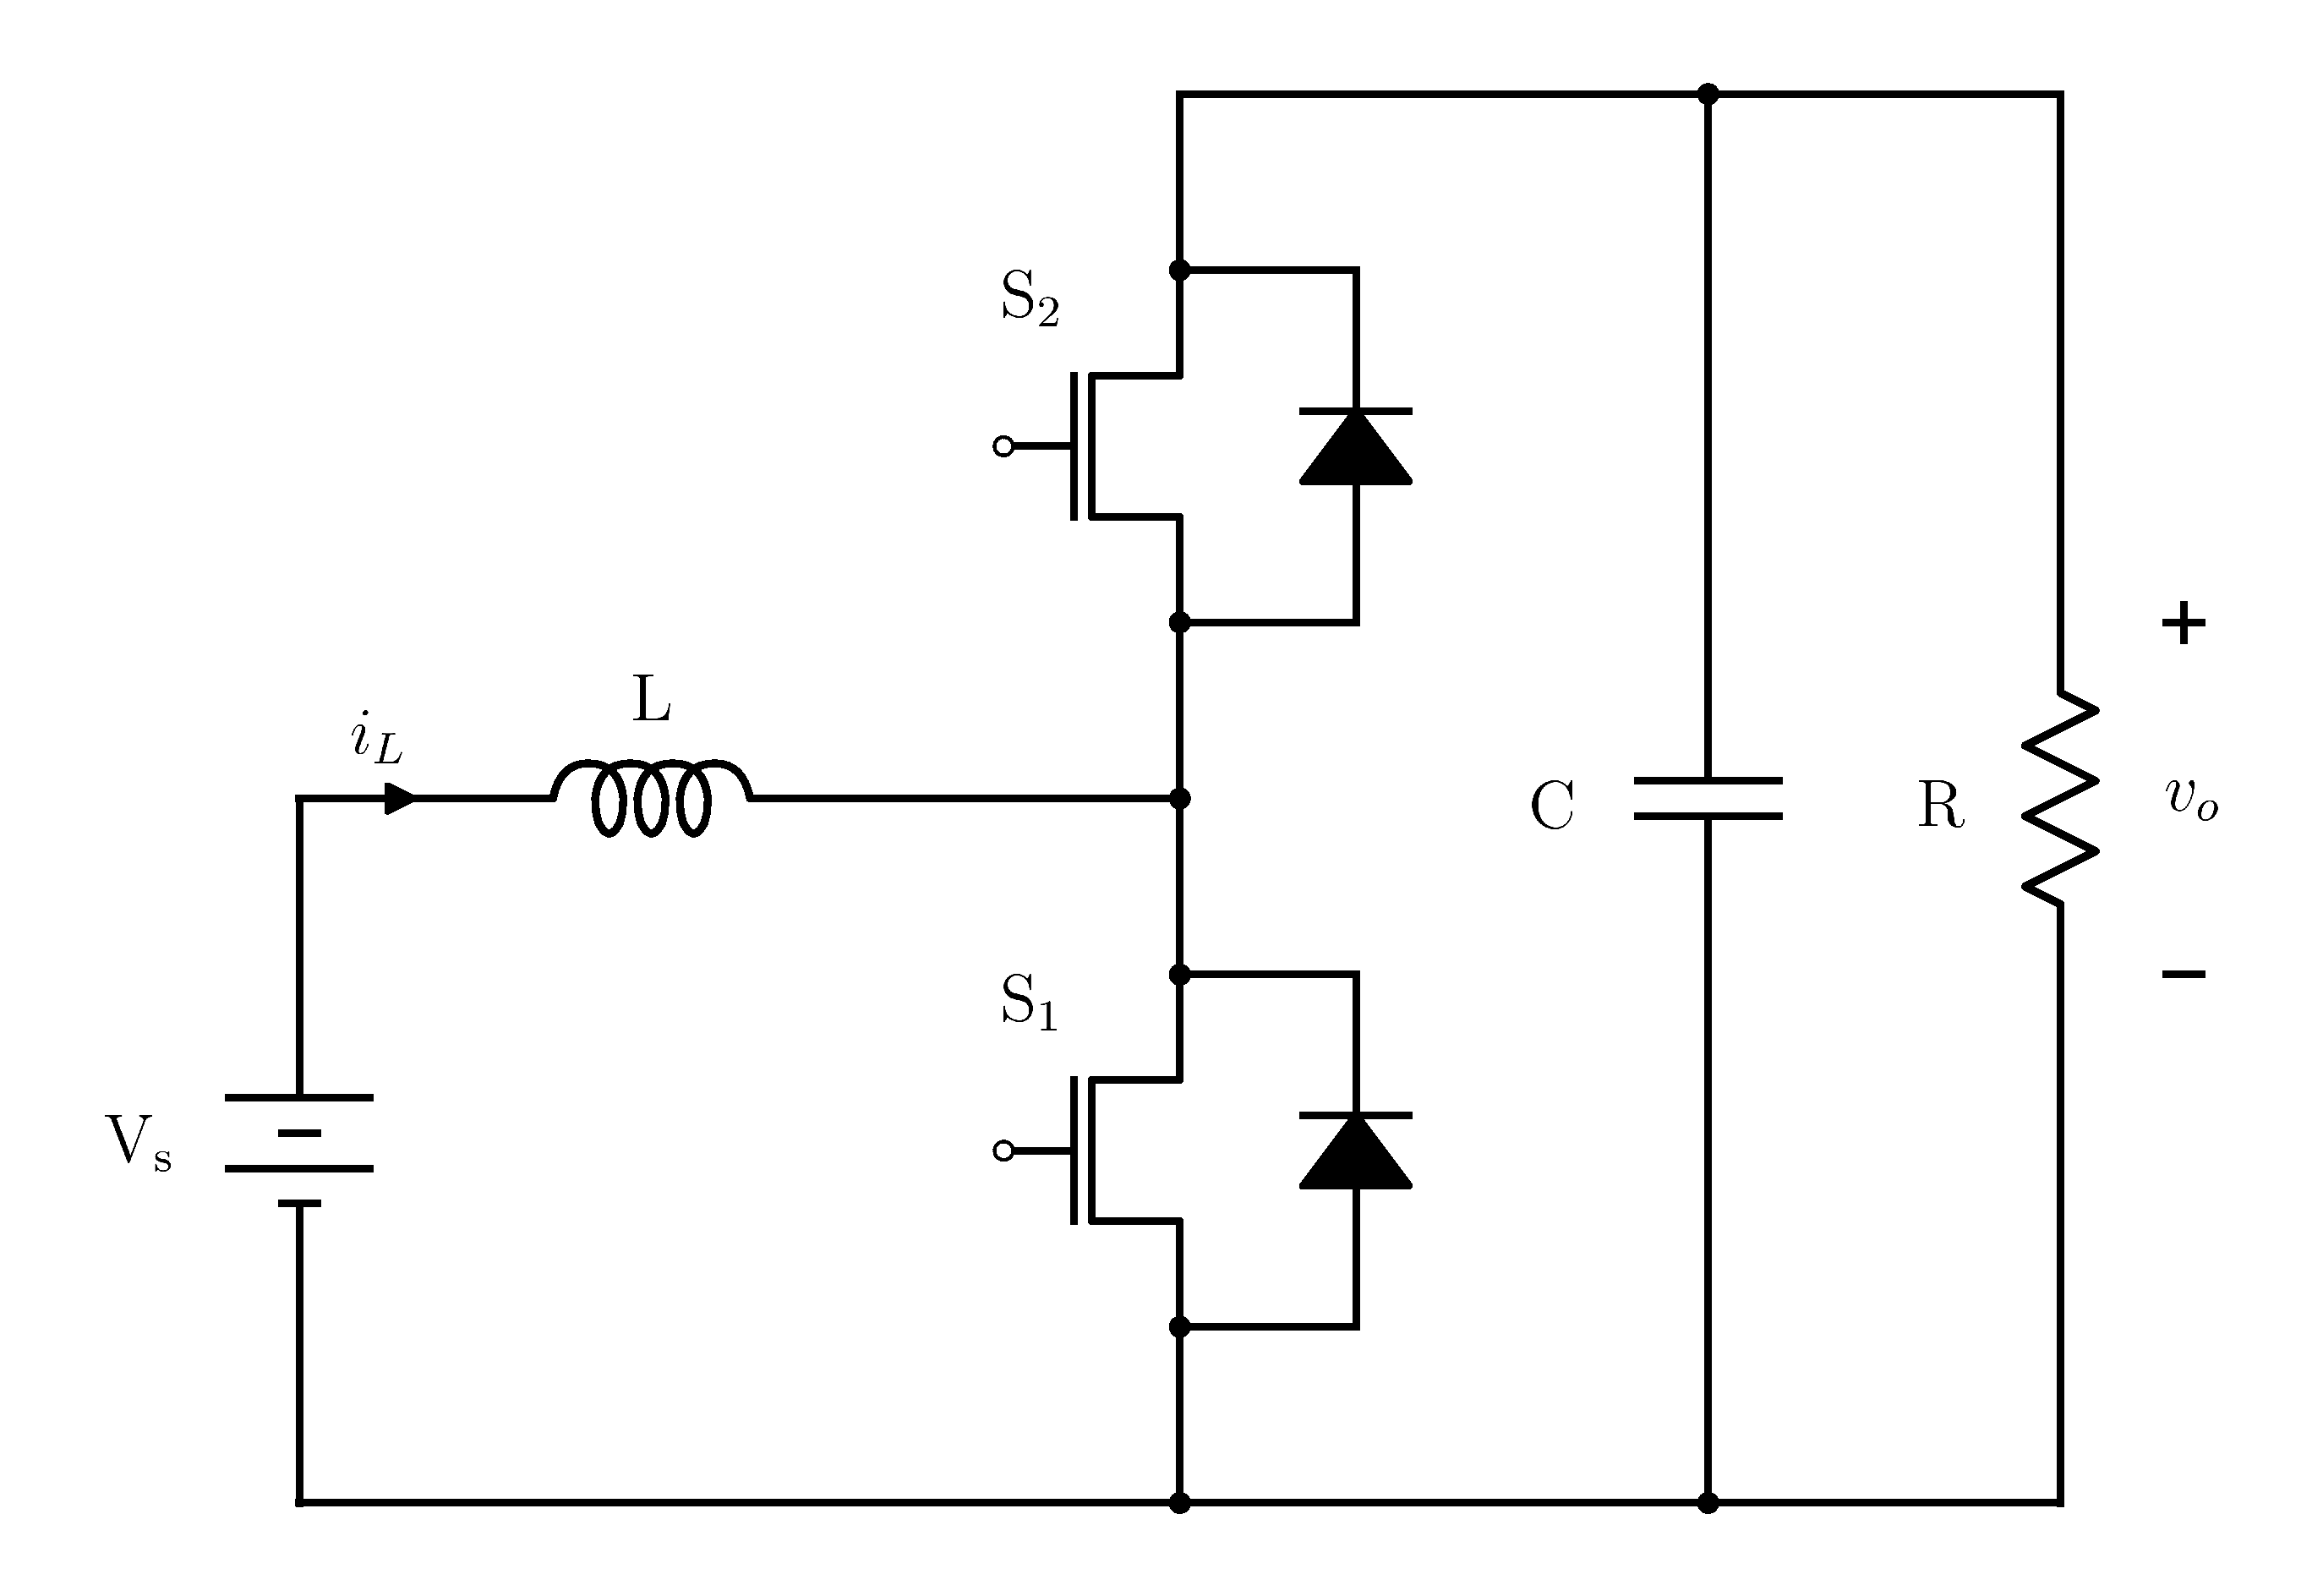
\includegraphics[width=0.46\columnwidth]{Imágenes/Diseño del control/Convertidor bidireccional de corriente.pdf}
  \caption{Convertidor elevador bidireccional en corriente.}
  \label{convertidor-bidireccional-diseno}
\end{figure} 

Las llaves $\mathrm{S_1}$ y $\mathrm{S_2}$ trabajan en forma complementaria: cuando $\mathrm{S_1}$ conduce, $\mathrm{S_2}$ no conduce, y viceversa. Con este pretexto y asumiendo que el convertidor se encuentra trabajando en modo de conducción continua (MCC), el mismo puede encontrarse en uno de los siguientes estados:

\begin{itemize}
    \item \textbf{$\boldsymbol{\mathrm{S_1}}$ conduce y $\boldsymbol{\mathrm{S_2}}$ no conduce}
    
    En este estado se analizan las ecuaciones de Kirchhoff para el circuito cerrado de la malla de la fuente y para las corrientes en el nodo de la carga. Expresándolas en función de la tensión en el inductor y la corriente por el capacitor, se obtienen las siguientes ecuaciones:

    \begin{equation}
        \begin{split}
          & L \frac{di_L(t)}{dt} = v_s(t) 
          \\
          & C \frac{dv_o(t)}{dt} = - \frac{v_o(t)}{R}
        \end{split}
        \label{sistema-modelo-1}
      \end{equation}

      \item \textbf{$\boldsymbol{\mathrm{S_1}}$ no conduce y $\boldsymbol{\mathrm{S_2}}$ conduce}
      
      Nuevamente expresando las ecuaciones de Kirchhoff correspondientes a este estado respecto la tensión en el inductor y la corriente en el capacitor se obtiene:
      
    \begin{equation}
        \begin{split}
          & L \frac{di_L(t)}{dt} = v_s(t) - v_o(t)
          \\
          & C \frac{dv_o(t)}{dt} = i_L(t)- \frac{v_o(t)}{R}
        \end{split}
        \label{sistema-modelo-2}
      \end{equation}
\end{itemize}

\subsection{Parametrizado mediante ciclo de trabajo}

Para unificar las Ecuaciones \ref{sistema-modelo-1} y \ref{sistema-modelo-2} hallados para el convertidor elevador en un solo sistema, se define la acción de control $u(t)$ de la siguiente forma:

\[
  u(t) = \left\{\begin{alignedat}{2}
    & 1 &\quad  \text{$S_1$ conduce y $S_2$ no conduce} \\
    & 0 &\quad  \text{$S_1$ no conduce y $S_2$ conduce} \\
  \end{alignedat}\right.
\]

Implementando esta condición para unir los sistemas de ecuaciones mencionados anteriormente se obtiene:

\begin{equation}
  \boxed{
    \begin{split}
      & L \frac{di_L(t)}{dt} = v_s(t) - \left[1-u(t)\right]v_o(t) \vspace{0.5cm}
      \\
      & C \frac{dv_o(t)}{dt} = \left[1-u(t)\right] i_L(t)- \frac{v_o(t)}{R}
  \end{split}
    }
  \label{sistema-modelo-param}
  \end{equation}

Este sistema de ecuaciones parametrizado es el típicamente usado para representar a los convertidores elevadores en la bibliografía de la temática.

\subsection{Promediado del sistema de ecuaciones}

En esta etapa se realiza una aproximación para poder simplificar las ecuaciones que definen el comportamiento de los mismos y así facilitar el tratamiento de los modelos resultantes.

Las Ecuaciones \ref{sistema-modelo-param} describen un \emph{sistema de estructura variable no lineal}, esto significa que el convertidor elevador se comporta como diferentes sistemas no lineales continuos en diferentes regiones de su estado de espacios, y este comportamiento se encuentra dictado por una acción de control $u(t)$ discontinua. Esto presenta una complejidad elevada en el análisis y control del sistema.

Una aproximación factible es el uso de \emph{medias móviles}, en las que cada señal se sustituye por su promedio durante un período de conmutación $T$. Este método permite modelar al sistema como uno de estructura no variable, debido a que la señal de control es continua bajo esta aproximación. Otra ventaja de las medias móviles es que al aplicarlo se obtiene la parte dominante de las señales y elimina las pequeñas perturbaciones, como el \emph{ripple} de conmutación, el cual no es de interés al diseñar el sistema de control para el conmutador.

Utilizando el método de promediado presentado en \cite{erickson} y \cite{hart} para simplificar las ecuaciones que rigen la dinámica del sistema:

\begin{equation}
  \left\langle x(t) \right\rangle_T = \frac{1}{T} \int_t^{t+T} x(\tau) \, d\tau
  \label{promediado}
\end{equation}

Puede demostrarse que aplicando la Ecuación \ref{promediado} a las Ecuaciones \ref{sistema-modelo-param} se obtiene:

\begin{equation}
  \boxed{
  \begin{split}
    & L \frac{d\left\langle i_L(t) \right\rangle_T}{dt} = \left\langle v_s(t) \right\rangle - \left[1-d(t)\right] \left\langle v_o(t) \right\rangle_T 
    \\
    & C \frac{d \left\langle v_o(t) \right\rangle_T}{dt} = \left[1-d(t)\right] \left\langle i_L(t) \right\rangle_T - \frac{\left\langle v_o(t) \right\rangle_T}{R}
  \end{split}
  }
  \label{sistema-modelo-prom}
\end{equation}

Siendo $d(t) = \left\langle u(t) \right\rangle_T$.

Cabe aclarar que es posible hallar un modelo promediado del convertidor trabajando en modo de conducción discontinua (MCD) \cite{jiansun}. Tal desarrollo no es presentado en este informe ya que escapa a los objetivos del presente trabajo.

\subsection{Linealización del sistema de ecuaciones}

Aún habiendo promediado al sistema, el modelo obtenido no es lineal, como se observa en las Ecuaciones \ref{sistema-modelo-prom} en las que aparecen productos entre los estados del sistema y la señal de control promediada $d(t)$. Como las técnicas tradicionales de análisis de sistemas (transformada de Laplace, diagramas de Bode, lugar de raíces, etc.) no son aplicables para el estudio de un modelo no lineal, es necesario linealizarlo.

Primero, ha de suponerse que el sistema ha sido llevado a un punto de trabajo fijo, en el que se encuentra con valores estacionarios en sus variables, a los que se hará referencia de la siguiente forma:

\begin{itemize}
  \item $I_{L_{ee}}$ es la \emph{corriente en la inductancia en estado estacionario}.
  \item $V_{o_{ee}}$ es la \emph{tensión en la salida en estado estacionario}.
  \item $V_{s_{ee}}$ es la \emph{tensión en la entrada en estado estacionario}.
  \item $D_{ee}$ es el \emph{ciclo de trabajo en estado estacionario}.
\end{itemize}

Al asumir que el sistema se encuentra en estado estacionario, las Ecuaciones \ref{sistema-modelo-prom} que definen la dinámica promedio del sistema se transforman en:

\begin{equation}
  \begin{split}
    & 0 = V_s - \left[ 1-D_{ee} \right] V_{o_{ee}}
    \\
    & 0 = \left[ 1-D_{ee} \right] I_{L_{ee}} - \frac{V_{o_{ee}}}{R}
  \end{split}
  \label{sistema-modelo-ee}
\end{equation}

Puede observarse que el comportamiento en este punto de trabajo coincide con el análisis efectuado en el capítulo de conversor elevador para modo de conducción continua, obteniéndose la misma relación de conversión (Ec. \ref{salida-elevador}).

Conocido el comportamiento del sistema en régimen de estado estacionario, se procede a la linealización del modelo. Este procedimiento consiste en realizar una aproximación de primer orden de las ecuaciones no lineales que describen al sistema, en un entorno muy cercano al punto de trabajo.

Para esto, primero debe construirse un \emph{modelo de pequeña señal} alrededor del punto de trabajo. Si se asume que el ciclo de trabajo promedio $d(t)$ es igual a un valor de estado estacionario $D$ más una perturbación denotada por $\hat{d}(t)$ se obtiene:

\begin{equation}
  \left\langle u(t) \right\rangle_T = d(t) = D_{ee} + \hat{d}(t)
  \label{ciclo-lineal} 
\end{equation}

Se asume que el valor de la perturbación $\hat{d}(t)$ es mucho menor que el valor de estado estacionario $D$, de modo que el valor promedio del ciclo de trabajo se mantendrá siempre cercano a este último. La respuesta del sistema ante esta perturbación de entrada resulta en los valores promedios de las variables:

\begin{equation}
  \begin{split}
    & \left\langle v_o(t) \right\rangle_T = V_{o_{ee}} + \hat{v_o}(t)
    \\
    & \left\langle i_L(t) \right\rangle_T = I_{L_{ee}} + \hat{i_L}(t)
  \end{split}
  \label{sistema-modelo-prom-ee}
\end{equation}

Las perturbaciones presentes en las Ecuaciones \ref{sistema-modelo-prom-ee} se consideran muy pequeñas con respecto a los valores de estado estacionario. Substituyendo los valores promedio definidos por las Ecuaciones~\ref{ciclo-lineal}~y~\ref{sistema-modelo-prom-ee} en el sistema promediado dado por las Ecuaciones \ref{sistema-modelo-prom}:

\begin{equation}
  \begin{split}
    & L \frac{d \left[ I_{L_{ee}} + \hat{i_L}(t)\right]}{dt} = V_s - \left[ 1 - D_{ee} - \hat{d}(t) \right] \, \left[ V_{o_{ee}} + \hat{v_o}(t) \right]
    \\
    & C \frac{d \left[ V_{o_{ee}} + \hat{v_o}(t)\right]}{dt} = V_s - \left[ 1 - D_{ee} - \hat{d}(t) \right] \, \left[ I_{L_{ee}} + \hat{i_L}(t) \right] - \left[ \frac{V_{o_{ee}}}{R} + \frac{\hat{v_o}(t)}{R} \right]
  \end{split}
\end{equation}

Operando:

\begin{equation}
  \begin{split}
    & L \frac{d \hat{i_L}(t)}{dt} = V_s -  (1 - D_{ee}) \, V_{o_{ee}} - (1 - D_{ee}) \, \hat{v_o}(t) + \hat{d}(t) V_{o_{ee}} + \hat{d}(t) \hat{v_o}(t)
    \\
    & C \frac{d \hat{v_o}(t)}{dt} = (1 - D_{ee}) \, I_{L_{ee}} + (1 - D_{ee}) \, \hat{i_L}(t) - \hat{d}(t) \, I_{L_{ee}} - \hat{d}(t) \, \hat{i_L}(t) - \frac{V_{o_{ee}}}{R} - \frac{\hat{v_o}(t)}{R}
  \end{split}
\end{equation}
Estas ecuaciones se simplifican considerando que:

\begin{itemize}
  \item $V_s = (1-D_{ee}) \, V_{o_{ee}}$
  \item $\frac{V_{o_{ee}}}{R} = I_{o_{ee}} = (1-D_{ee}) \, I_{L_{ee}}$
  \item Se eliminan los términos no lineales de segundo orden que se presentan al considerarse que las perturbaciones son muy pequeñas, y el producto entre ellas lo son aún más.
\end{itemize}

El resultado es el modelo lineal del convertidor:

\begin{equation}
  \boxed{
  \begin{split}
  & L \frac{d\hat{i_L}(t)}{dt} = - (1-D_{ee}) \, \hat{v_o}(t) + \hat{d}(t) \, V_{o_{ee}}
  \\ 
  & C \frac{d\hat{v_o}(t)}{dt} = - (1-D_{ee}) \, \hat{i_L}(t) - \hat{d}(t) \, I_{L_{ee}} - \frac{\hat{v_o}(t)}{R}  
  \end{split}
  }
  \label{sistema-modelo-lineal}
\end{equation}

\section{Diseño del sistema de control}

El primer paso en el diseño del sistema de control consiste en definir qué tipo de señal se utilizará como excitación en el gate de los transistores del convertidor. Dos alternativas son presentadas:

\begin{itemize}
  \item Los \textbf{sistemas de control a frecuencia fija} poseen un ciclo de trabajo variable, pero la frecuencia es constante. Un ejemplo es la modulación por ancho de pulso o PWM (del inglés \emph{pulse width modulation}).
  \item Los \textbf{sistemas de control a frecuencia variable} mantienen constante el tiempo durante el cual el transistor es excitado con un nivel alto, pero la frecuencia de su conmutación es variable. Un ejemplo es la modulación de la frecuencia del pulso o PFM (del ingles \emph{pulse frequency modulation}).
\end{itemize}

El control por PWM presenta una menor eficiencia que el control por PFM con cargas pequeñas, debido a que este último reduce la frecuencia de su señal en estos casos, lo que conlleva menores pérdidas por conmutación de las llaves. Aun así, el control por PWM es preferible debido a su frecuencia fija, lo que significa que el \emph{ripple} de conmutación se encuentra acotado, y simplifica de gran manera la implementación de la acción de control, mientras que en el control por PFM el rizado puede tener amplitudes mayores cuando se reduce mucho la frecuencia. Por esta razón se utiliza este un control con señal de modulación de ancho de pulso para este trabajo.

El siguiente paso es comenzar a diseñar la estrategia de control, la cual se verá afectada por las especificaciones disponibles en cuanto a modos de funcionamiento y las características de la respuesta dinámica requerida. Específicamente para este trabajo, el objetivo de la acción de control es mantener una tensión constante en la carga.

Proponiendo un lazo de realimentación como el de la Figura \ref{lazo-tension-propuesto}, se observa rápidamente que esta estrategia no es viable cuando la planta es un convertidor elevador.

\begin{figure}[hbt!]
  \centering
  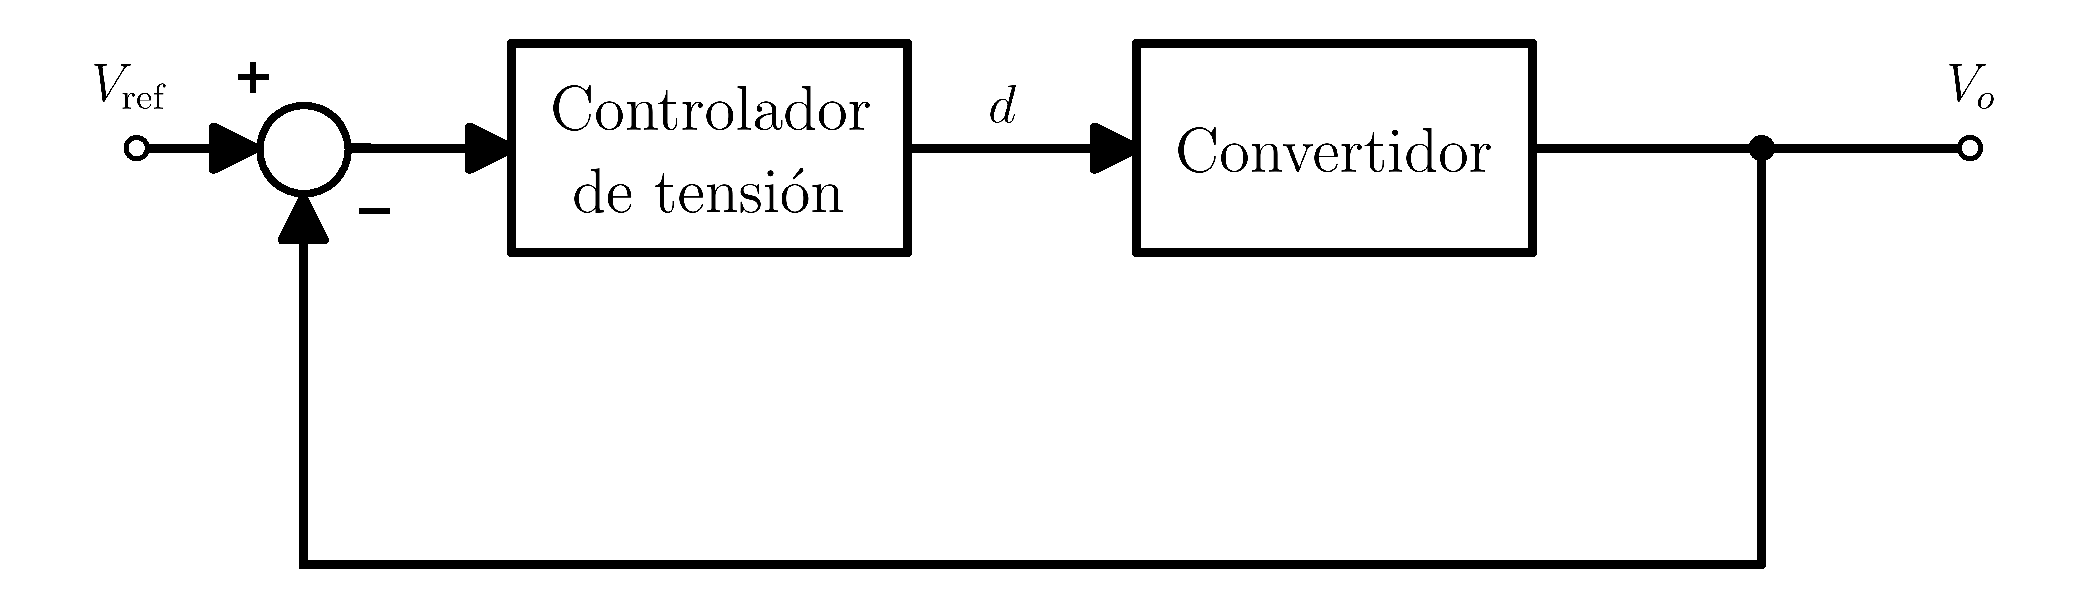
\includegraphics[width=0.65\columnwidth]{Imágenes/Diseño del control/Primer lazo de control de tensión.pdf}
  \caption{Ilustración del lazo de control de tensión propuesto.}
  \label{lazo-tension-propuesto}
\end{figure} 

Esta impracticabilidad se demuestra asumiendo inicialmente que la tensión de salida se ha estabilizado en un valor estacionario $V_{o_{ee}}$ y considerando una tensión de entrada constante $V_s$. Substituyendo estos valores en las Ecuaciones \ref{sistema-modelo-prom} correspondientes al sistema promediado:

\begin{equation*}
  \begin{split}
    & L \frac{d\left\langle i_L(t) \right\rangle_T}{dt} = V_s - \left[1-d(t)\right] \, V_{o_{ee}}
    \\
    & 0 = \left[1-d(t)\right] \left\langle i_L(t) \right\rangle_T - \frac{V{o_{ee}}}{R}
  \end{split}
\end{equation*}

Realizando un reemplazo sobre el ciclo de trabajo promediado se obtiene:

\begin{equation}
  L \frac{d\left\langle i_L(t) \right\rangle_T}{dt} = V_s - \frac{V_{o_{ee}^2}}{R \, \left\langle i_L(t) \right\rangle_T}
  \label{prueba-inestabilidad-lazo}
\end{equation}

Y efectuando otro reemplazo con la potencia de salida $P_{o_{ee}} = V_{o_{ee}}^2/R$ se obtiene:

\begin{equation*}
  L \frac{d\left\langle i_L(t) \right\rangle_T}{dt} = V_s - \frac{P_{o_{ee}}}{\left\langle i_L(t) \right\rangle_T}
\end{equation*}

Dado que la potencia de salida es siempre menor a la de la entrada debido a pérdidas, se tiene:

\begin{equation*}
  \frac{P{o_{ee}}}{\left\langle i_L(t) \right\rangle_T} < \frac{P{s_{ee}}}{\left\langle i_L(t) \right\rangle_T}
\end{equation*}

\begin{equation*}
  \boxed{\frac{P{o_{ee}}}{\left\langle i_L(t) \right\rangle_T} < V_s \quad \forall \quad t}
\end{equation*}

Esto implica que el miembro derecho de la Ecuación \ref{prueba-inestabilidad-lazo} es mayor que cero para todo instante de tiempo, por lo que la derivada de la corriente es siempre positiva, y en consecuencia la corriente por el inductor diverge. 

La razón por la que esto ocurre es que hay una parte de la dinámica del sistema que no está siendo controlada. Es decir, si solamente se controla la tensión de salida, la corriente por el inductor se deja variar en forma libre. Esta dinámica de lazo cerrado para estados no controlados de un sistema no lineal se conoce como \emph{dinámica escondida} o \emph{dinámica cero}, y su estabilidad es condición necesaria para la estabilidad del sistema entero \cite{dynamics}. Dado que la dinámica cero del convertidor con un lazo cerrado de tensión resulta inestable, se concluye que es necesario implementar un control de corriente anidado dentro del lazo de tensión. En resumen, la estrategia de control consiste en:

\begin{enumerate}
  \item El \textbf{lazo interno de control de corriente}, el cual se encarga de la dinámica escondida de esta variable de estado.
  \item El \textbf{lazo externo de control de tensión}, el cual se encarga de generar la acción de control para cumplir el objetivo de mantener la tensión de carga constante. Este lazo es el encargado de calcular e inyectar la referencia en el lazo interno.
\end{enumerate}

Por eso mismo, se realizará un diseño en fases para cumplir individualmente estos objetivos, cuya primer etapa será el diseño del lazo interno de corriente.

\subsection{Diseño del lazo interno de corriente}

Dado el contexto de un sistema de control de tensión, para el diseño del lazo de corriente se asume una tensión constante, y se controla el flujo de la potencia en forma indirecta mediante el control de la componente media de la corriente por el inductor. 

La Figura \ref{lazo-corriente} representa el modo de control propuesto para la corriente del convertidor electrónico. Este consiste en un lazo de realimentación que permite comparar la corriente en el inductor con la referencia de corriente deseada, para inyectar con la señal error resultante a un controlador en cascada con el sistema.

\begin{figure}[hbt!]
  \centering
  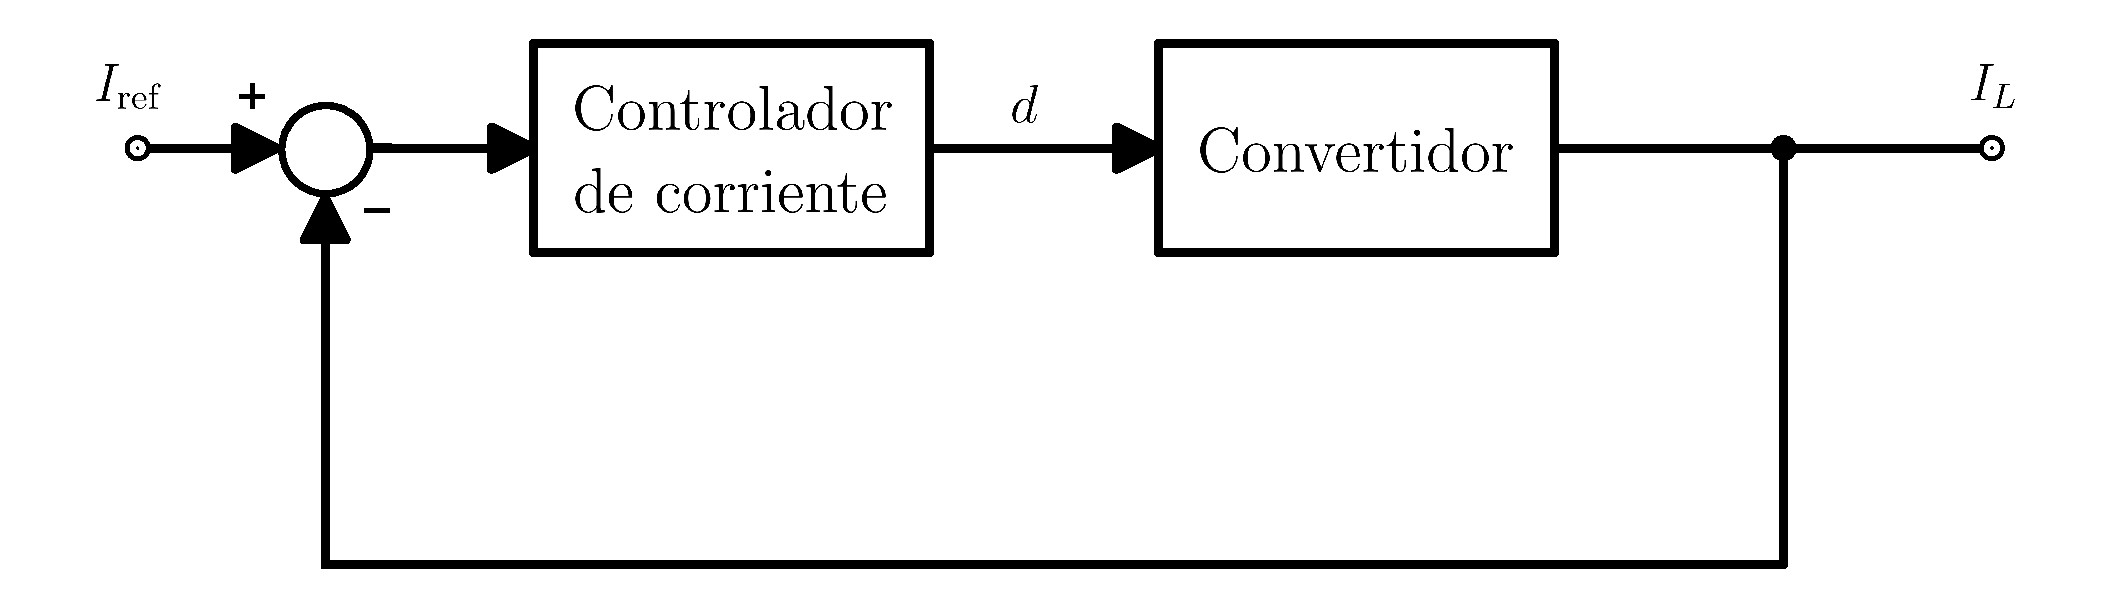
\includegraphics[width=0.65\columnwidth]{Imágenes/Diseño del control/Lazo de control de corriente.pdf}
  \caption{Ilustración del lazo de control de corriente.}
  \label{lazo-corriente}
\end{figure} 

El modelo linealizado del convertidor elevador obtenido en las Ecuaciones \ref{sistema-modelo-lineal} permite aplicar herramientas convencionales de análisis como la transformada de Laplace, lugar de raíces, entre otros. Por su parte, como se aclaró en el Capítulo \ref{cap-fpga}, el hardware de control será un FPGA, el cual opera a partir de muestras obtenidas mediante dos conversores. Por esto mismo, el diseño del controlador se realiza en el dominio discreto.

El primero paso a realizar es obtener la función de transferencia continua del convertidor, aplicando la transformada de Laplace a las Ecuaciones \ref{sistema-modelo-lineal}, y asumiendo que las condiciones iniciales son nulas. Las siguientes ecuaciones son obtenidas

\begin{equation}
  \begin{split}
    & s \, L \, I_L(s) = - \left( 1 - D_{ee} \right) \, V_o(s) + V_{o_{ee}} \, D(s)
    \\
    & s \, C \, V_o(s) = - \left( 1 - D_{ee} \right) \, I_L(s) + I_{L_{ee}} \, D(s) - \frac{V_o(s)}{R}
    \label{sistema-modelo-laplace}
  \end{split}
\end{equation}

Considerando como salida a la corriente del inductor $I_L$ y como entrada al ciclo de trabajo $D$, se obtiene la función de transferencia expresada en la Ecuación \ref{transferencia-corriente-inductor}.

\begin{equation}
  \boxed{G_{I_L}(s) = \frac{I_L(s)}{D(s)} = \frac{\frac{V_{o_{ee}}}{L} \, s + \left[ \frac{I_{L_{ee} \, (1 - D_{ee})}}{L \, C} + \frac{V_{o_{ee}}}{L\,C\,R} \right]}{s^2 + \frac{1}{R\,C} \, s + \frac{\left( 1 - D_{ee} \right)^2}{L \, C}}}
  \label{transferencia-corriente-inductor}
\end{equation}

Ahora, deben seleccionarse valores de tensión de entrada $V_s$, ciclo de trabajo $D_{ee}$, y resistencia de carga $R$ que conforman el punto de operación alrededor del cual se trabajará con el sistema. Considerando una tensión un poco menor de la nominal del banco de supercapacitores y baterías de litio, se obtiene la asignación mostrada en la Tabla \ref{punto-trabajo-convertidor}.

\begin{table}[hbt!]
  \centering
  \begin{tabular}{l|l}
  $V_s$     & \SI{25}{\volt} \\
  $D_{ee}$    & 0.5 \\
  $R$        & \SI{15}{\ohm}  \\
  $V_{o_{ee}}$ & \SI{50}{\volt} 
  \end{tabular}
  \caption{Punto de trabajo alrededor del cual se linealiza el convertidor}
  \label{punto-trabajo-convertidor}
\end{table}

En el convertidor elevador utilizado, los valores de inductancia y capacitancia por diseño son de \SI{200}{\micro\henry} y \SI{200}{\micro\farad}, respectivamente. Con estos valores y reemplazando en la Ecuación \ref{transferencia-corriente-inductor}:

\begin{equation}
  \boxed{G_I(s) = \frac{I_L(s)}{D(s)} = \frac{250\,000\,s + 15.15 \times 10^6}{s^2 + 30.3 \, s + 568.18 \times 10^3}}
  \label{planta-valores}
\end{equation}

Cuyos polos complejos conjugados se encuentran en -15.15 $\pm$ $j$753.62. 

La discretización de la planta depende del tiempo de muestreo $T_s$ de los conversores analógico-digitales, el cual debe ser varias veces menor que la menor constante de tiempo del sistema. Para esto, se programa al controlador de los ADCs para que tengan un período de muestreo de \SI{1.6}{\micro\second}, bien por debajo del período de conmutación de las llaves de \SI{50}{\micro\second}. La aproximación utilizada para la discretización de la planta es el método de \emph{Euler en avance}:

\begin{equation}
  s = \frac{z-1}{T_s}
  \label{euler-avance}
\end{equation}

En donde $T_s$ es el período de muestreo anteriormente mencionado. Reemplazando la Ecuación \ref{euler-avance} en la Ecuación \ref{planta-valores}:

\begin{equation}
  \boxed{G_I(z) = \frac{0.4(z-0.999903)}{z^2 - 1.99995z  + 0.999953}}
  \label{modelo-discretizado}
\end{equation}

Una vez obtenido el modelo discretizado, es necesario seleccionar el tipo de controlador a implementar. Las especificaciones buscadas en cuanto la respuesta dinámica de la corriente en el inductor son:

\begin{itemize}
  \item Error de estado estacionario nulo.
  \item Tiempo de establecimiento del orden del milisegundo o menor.
  \item Si se producen sobrepicos, que su amplitud no ponga en riesgo a los componentes del sistema, ni a la carga.
\end{itemize}

Se optó por la implementación de un control tipo proporcional-integral-derivativo digital, más comúnmente llamados por su acrónimo \emph{controlador PID}.

\subsubsection{Controladores PID}
\label{diseno-controladores-pid}

Los controladores PID (Figura \ref{esquema-pid}) son controladores que tienen una larga historia en el campo de control automático. Debido a su mecanismo intuitivo y su relativa simpleza, además de una performance satisfactoria en un amplio rango de procesos, se consideran el controlador estándar en la industria. Aplicar una ley de control PID consiste en aplicar la suma de tres tipos de acciones de control: una acción proporcional, una integral, y una derivativa.

\begin{figure}[hbt!]
  \centering
  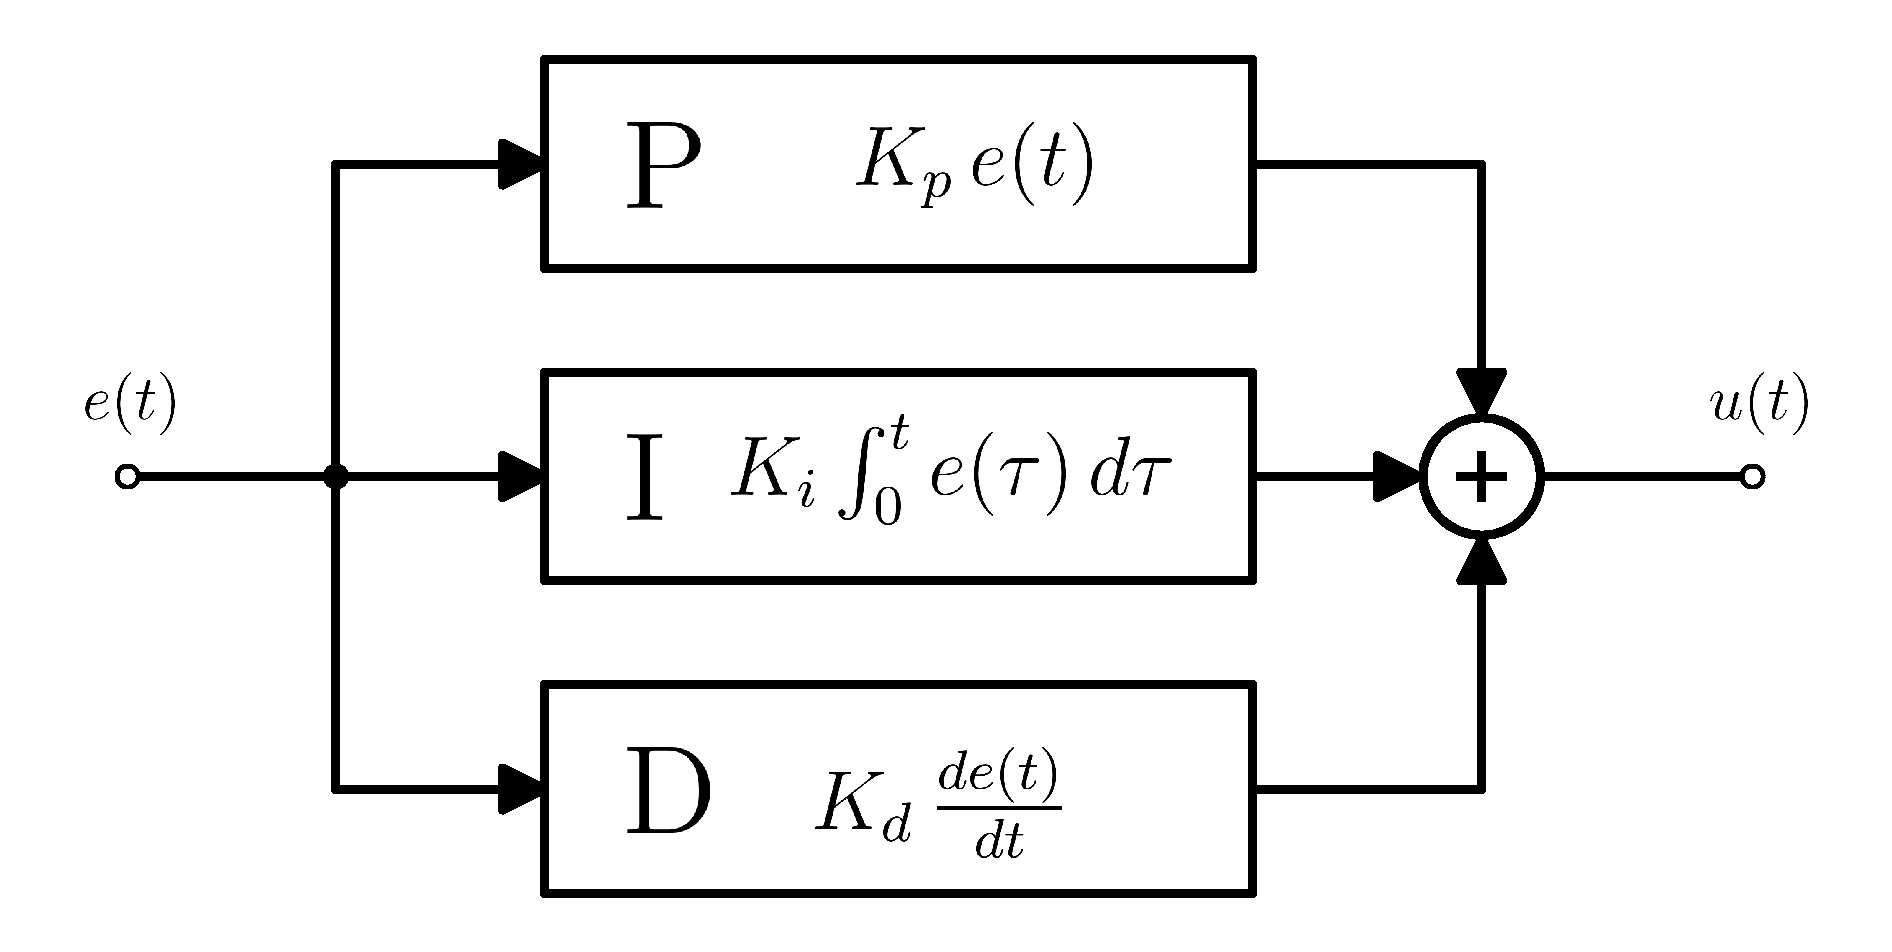
\includegraphics[width=0.45\columnwidth]{Imágenes/Diseño del control/Controlador PID.pdf}
  \caption{Diagrama en bloques de un controlador PID.}
  \label{esquema-pid}
\end{figure} 

\begin{itemize}
  \item La \textbf{acción proporcional} es proporcional a la señal error que ingresa al controlador, dada por la expresión
  \begin{equation*}
    u(t) = K_p \, e(t) = K_p \left( r(t) - y(t) \right)
  \end{equation*}
  en donde $K_p$ es la ganancia proporcional. Su significado es sencillo, ya que su comportamiento es aumentar la variable de control cuando el error es grande, con su signo apropiado. La mayor desventaja de usar un controlador proporcional puro es que produce un error de estado estacionario, aún cuando la planta presente una dinámica integral (es decir, su función de transferencia presenta un polo en el origen del plano complejo).
  \item La \textbf{acción integral} es proporcional a la integral del error del control, es decir
  \begin{equation*}
    u(t) = K_i \, \int_{0}^{t} e(\tau) \, d\tau
  \end{equation*}
  en donde $K_i$ es la ganancia integral, y su función de transferencia es:
  \begin{equation*}
    C(s) = \frac{K_i}{s}
  \end{equation*}

  La presencia del polo en el origen permite la reducción a cero del error de estado estacionario cuando una señal escalón es aplicada en la referencia o cuando ocurre una perturbación en la carga. Aún así, cuando se presenta una acción integral, el llamado efecto \emph{windup} puede ocurrir en el caso de que se presente una saturación en la variable de control.

  Esta situación se da debido a que el integrador del controlador no conoce los límites físicos del sistema a controlar y por lo tanto, ante ciertas situaciones (por ejemplo, un gran cambio en la referencia), es posible que la acción de control generada exceda estas limitaciones, lo que puede causar un sobrepico en alguna variable de estado del sistema. Para evitar este problema se utilizan métodos \emph{anti-windup}.
  \item Mientras la acción proporcional se basa en el valor presente del error de control y la acción integral se basa en sus valores pasados, la \textbf{acción derivativa} se basa en predecir futuros valores de esta señal. Una ley de control derivativa ideal puede ser expresada como:
  \begin{equation*}
    u(t) = K_d \, \frac{d e(t)}{dt}
  \end{equation*}
  en donde $K_d$ es la ganancia derivativa, y su función de transferencia es 
  \begin{equation*}
    C(s) = K_d \, s 
  \end{equation*}
  Este tipo de acción de control tiene un gran potencial en mejorar la performance del control, debido a que podría anticipar una incorrecta tendencia en la señal error y contrarrestarla. Sin embargo, también posee algunas cuestiones críticas que hacen que no sea adoptada en casos prácticos. Específicamente en el marco de este trabajo y debido a la conmutación de las llaves y la generación del ripple presente en las variables de estado a controlar, el término derivativo termina amplificando este rizado, lo cual es indeseado y podría generar una oscilación en el sistema de control. Por esto mismo, se decide implementar un controlador proporcional-integral (PI).
\end{itemize}

La transferencia discreta de un PI suele expresarse como: 

\begin{equation*}
  \mathrm{PI}_I(z) = K_p + \frac{K_i \, T_s}{z-1}
\end{equation*}

Y las ganancias proporcional e integral $K_p$ y $K_i$ deben ser balanceadas a partir de la sintonización del controlador PI para obtener la performance buscada a lazo cerrado. En la Sección \ref{implementacion-pid} del Capítulo \ref{implementacion-control} se detalla la implementación del método de \emph{anti-windup} para la acción de control integral, conocido como \emph{clamping}. El clamping consiste en deshabilitar el integrador cuando una cierta condición es alcanzada. Las siguientes opciones pueden ser implementadas:

\begin{itemize}
  \item El término integral se limita a un valor predefinido.
  \item La integración se detiene cuando el error es mayor a un umbral predefinido, es decir, cuando la variable de estado del proceso está muy lejos de la referencia.
  \item La integración se detiene caundo la variable de control se satura, es decir, cuando $u \neq u'$.
  \item La integración se detiene cuando la variable de control se satura, y tiene la misma señal que la señal error, es decir, cuando $u \cdot e > 0$.
\end{itemize}

El método utilizado en este trabajo es el primero, en el cual se realiza una saturación del término integral.

\subsubsection{Filtro de corriente}
\label{diseno-filtro-corriente}

Como se mencionó anteriormente, la acción de control será calculada a partir de la corriente media por el inductor, y no su valor instantáneo. Por esto mismo resulta necesario aplicar a la señal de corriente medida un filtro pasa-bajo que rechace las componentes del \emph{ripple}, y que además sea lo suficientemente rápido para poder seguir la dinámica de la planta modelada en la Ecuación \ref{planta-valores}. Dado que este rizado es producto de la conmutación de las llaves y su frecuencia fundamental es de \SI{20}{\kilo\hertz}, y los polos de la planta poseen un valor absoluto aproximado de 750, se decide implementar un filtro pasabajos de primer orden con frecuencia de corte en \SI{1.5}{\kilo\hertz}. La Figura \ref{filtro-corriente} muestra la forma en la que se incorpora este filtro al lazo interno de realimentación de corriente.

\begin{figure}[hbt!]
  \centering
  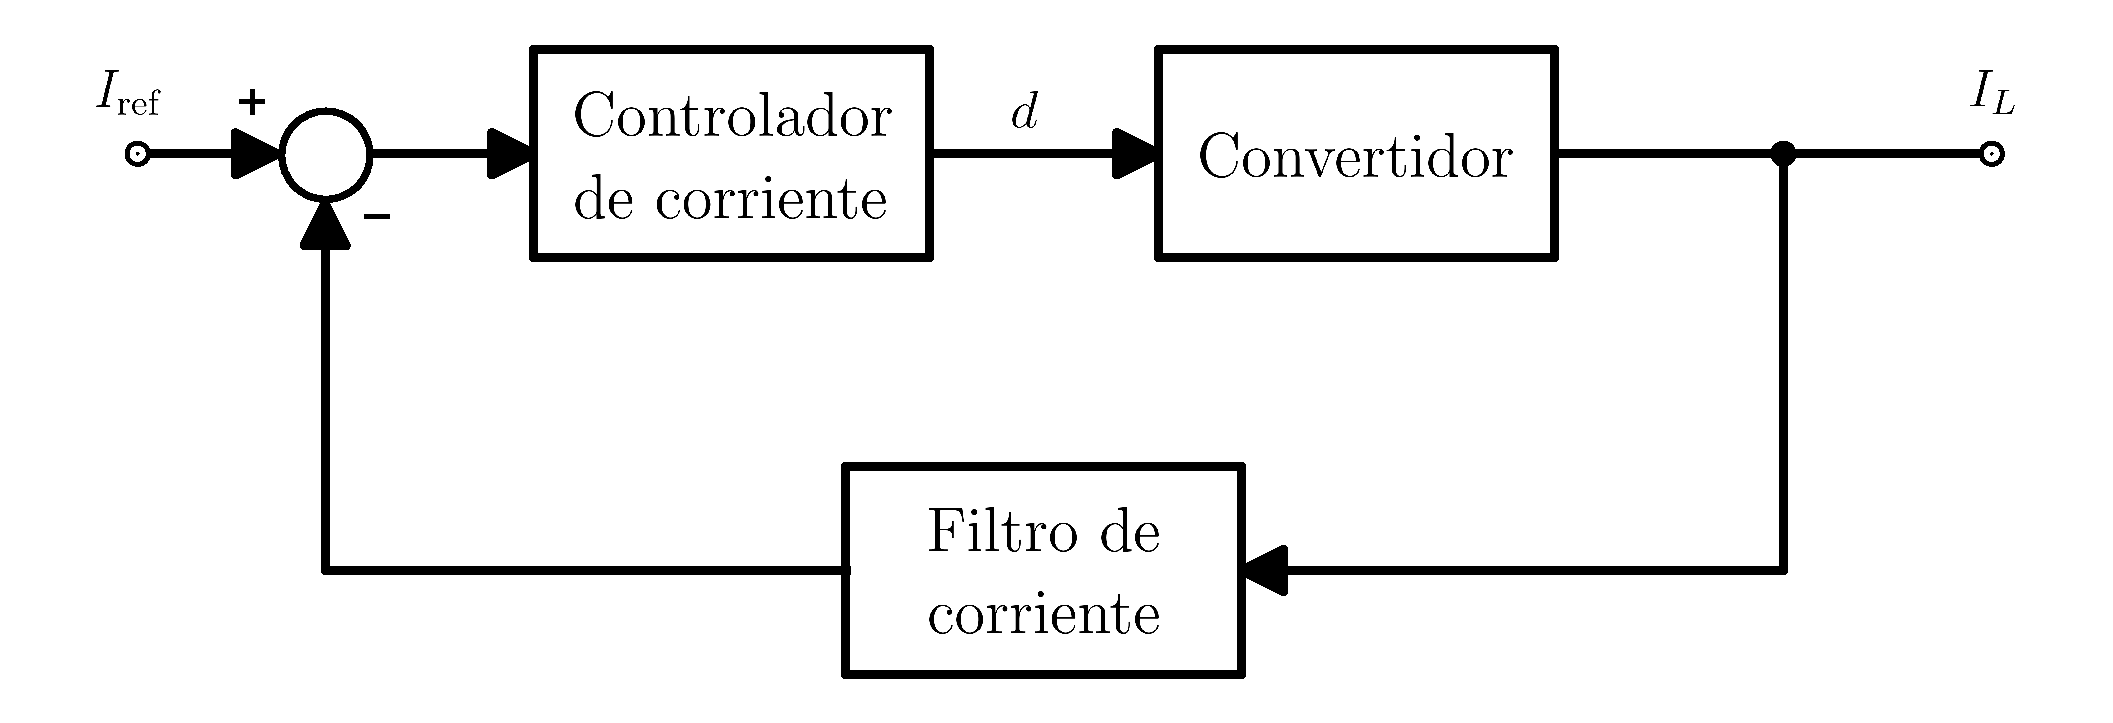
\includegraphics[width=0.65\columnwidth]{Imágenes/Diseño del control/Lazo de control de corriente con filtro.pdf}
  \caption{Lazo de control de corriente con filtro pasa-bajo.}
  \label{filtro-corriente}
\end{figure} 

Para esto, se partió de la transferencia en continua del filtro de primer orden a implementar:

\begin{equation}
  F_I(s) = \frac{\omega_c}{s+\omega_c} = \frac{2\pi \, 1.5 \times 10^3 }{s+ 2\pi \, 1.5 \times 10^3}
\end{equation}

Y luego se transformó al dominio discreto, nuevamente mediante el método de Euler en avance y la frecuencia de muestreo establecida anteriormente:

\begin{equation}
  \boxed{F_I(z) = \frac{0.0150796}{z-0.98492}}
  \label{filtro-corriente-discretizado}
\end{equation}

\subsubsection{Simulación del lazo interno de corriente}

Luego de filtrar correctamente la corriente por el inductor del convertidor, se procede al ajuste de los parámetros del controlador proporcional-integral. Para ello, la sintonización inicial fue hecha a partir de la transferencia lineal encontrada en la Ecuación \ref{modelo-discretizado} y las herramientas de simulación y cálculo provistas por MATLAB\textsuperscript\textregistered \hspace{0.6pt} y Simulink\textsuperscript\textregistered.

En la Figura \ref{simulacion-modelo-discretizado-corriente} puede observarse el esquema realizado para una primer simulación respecto de la transferencia discretizada del modelo. Para este paso fue utilizada la herramienta de sintonización provista por Simulink\textsuperscript\textregistered, la cual cuenta con dos controles deslizantes (Figura \ref{tuner-modelo-discretizado-corriente}) los cuales permiten ajustar la rapidez de la respuesta temporal y el comportamiento transitorio de la acción de control, y en base a eso, generar los parámetros del controlador.

\begin{figure}[hbt!]
  \centering
  \includegraphics[width=0.55\columnwidth]{Imágenes/Diseño del control/Simulación del lazo de corriente/Primer simulación del lazo de corriente.pdf}
  \caption{Primer simulación del lazo de control de corriente.}
  \label{simulacion-modelo-discretizado-corriente}
\end{figure} 

\begin{figure}[hbt!]
  \centering
  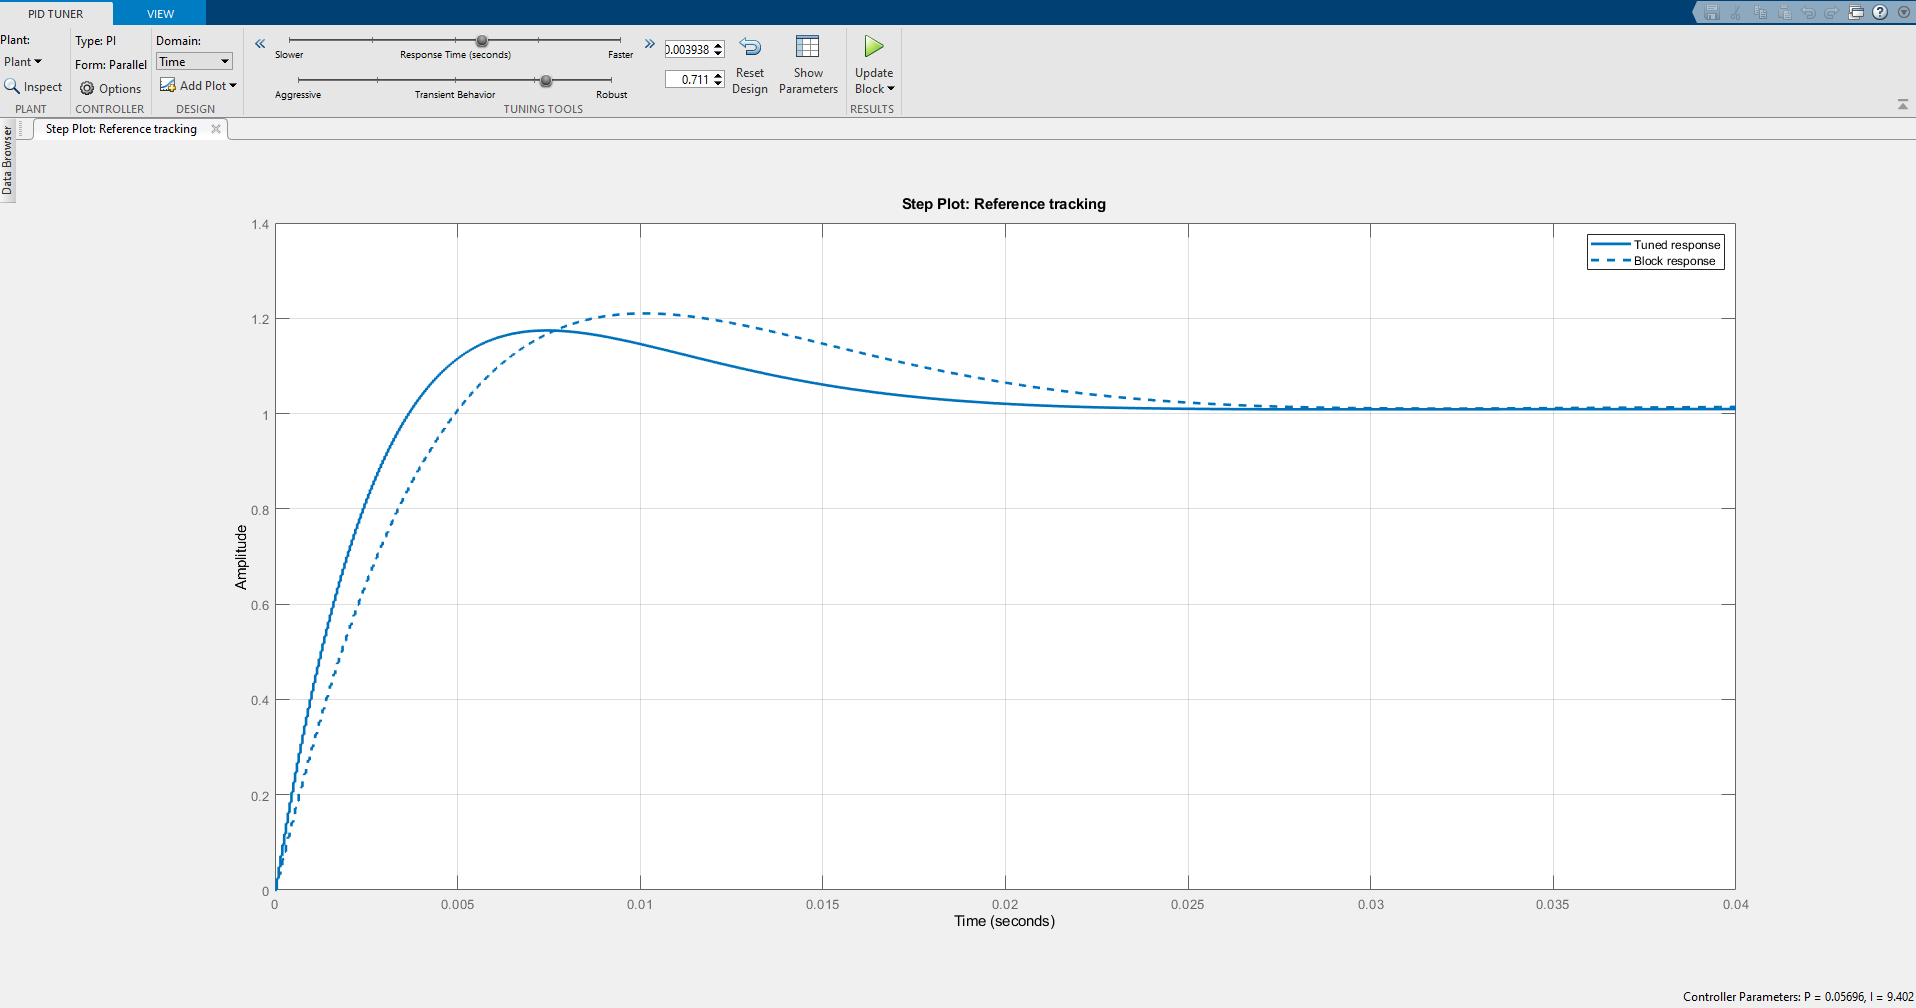
\includegraphics[width=0.70\columnwidth]{Imágenes/Diseño del control/Simulación del lazo de corriente/Tuner de Simulink.png}
  \caption{Sintonización del PI mediante herramientas de Simulink\textsuperscript\textregistered.}
  \label{tuner-modelo-discretizado-corriente}
\end{figure} 

Una vez generada una primer aproximación del lazo de control con una respuesta satisfactoria, se reemplaza al modelo linealizado del convertidor por el modelo real parametrizado, expresado por las Ecuaciones \ref{sistema-modelo-param}, y se implementa el filtro de corriente, como se observa en la Figura \ref{simulacion-modelo-real-corriente}. En esta simulación se inyecta un escalón unitario de \SI{8}{\ampere} a \SI{9}{\ampere} en la referencia del lazo de control de corriente y se observan las variables de estados del convertidor (corriente por el inductor y tensión en el capacitor o de salida), además de corroborar el funcionamiento del filtro implementado.

Analizando el comportamiento transitorio obtenido con la simulación del modelo real y realizando nuevos ajustes de manera de obtener una performance satisfactoria, se llega al siguiente controlador:

\begin{equation*}
  \boxed{\mathrm{PI}_I (z) = 0.02 + \frac{12 \cdot 1.6 \times 10^{-6}}{z-1}}
\end{equation*}

Donde se deduce que la constante proporcional $K_p$ es 0.02, y la constante integral $K_i$ es 12.

\begin{figure}[hbt!]
  \centering
  \includegraphics[width=0.72\columnwidth]{Imágenes/Diseño del control/Simulación del lazo de corriente/Simulación real del lazo de corriente.pdf}
  \caption{Simulación real del lazo de control de corriente.}
  \label{simulacion-modelo-real-corriente}
\end{figure} 

En la Figura \ref{formas-onda-lazo-corriente} se grafican los resultados de la simulación. A partir de la corriente por el inductor filtrada (Figura \ref{formas-onda-lazo-corriente}c), la cual atenúa satisfactoriamente al rizado de la forma de onda, se realiza un análisis del transitorio del escalón unitario aplicado. Utilizando las herramientas provistas por Simulink\textsuperscript\textregistered, se mide un valor de sobrepico del 1.8\% respecto del valor de estado estacionario de \SI{9}{\ampere}, y un tiempo de establecimiento con criterio del 2\%\footnote{Se entiende como \emph{tiempo de establecimiento del 2\%} al tiempo que tarda la señal en situarse en un entorno del 2\% alrededor del valor de estado estacionario.} de aproximadamente \SI{1}{\milli\second}.

En la Figura \ref{formas-onda-filtradas-lazo-corriente} se observa con mayor detalle la acción del filtro alrededor del punto de salto del escalón.

\begin{figure}[hbt!]
  \centering
  \subfloat[Referencia de corriente.]{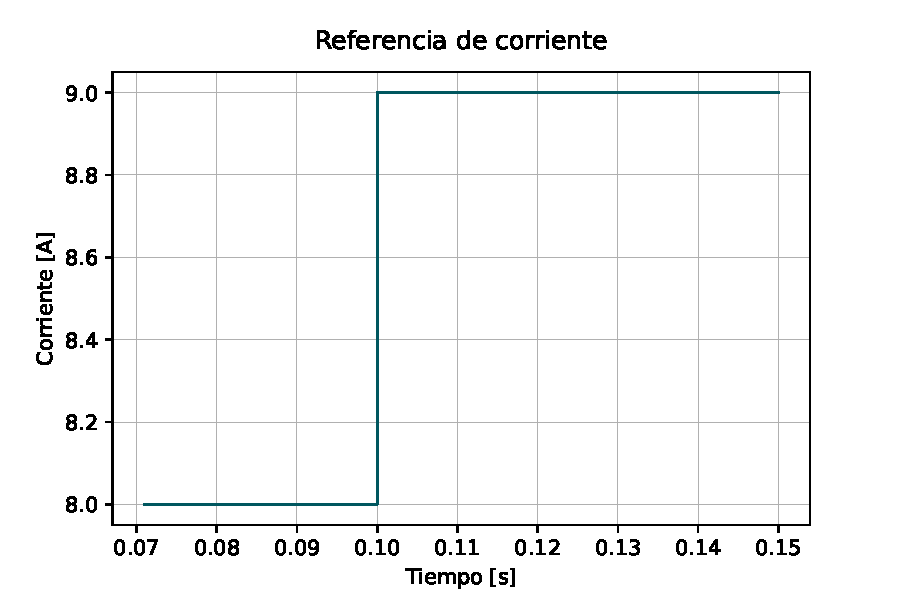
\includegraphics[width=0.45\textwidth]{Imágenes/Diseño del control/Simulación del lazo de corriente/Referencia de corriente.pdf}}    
  \hspace{3.5mm}
  \subfloat[Corriente por el inductor.]{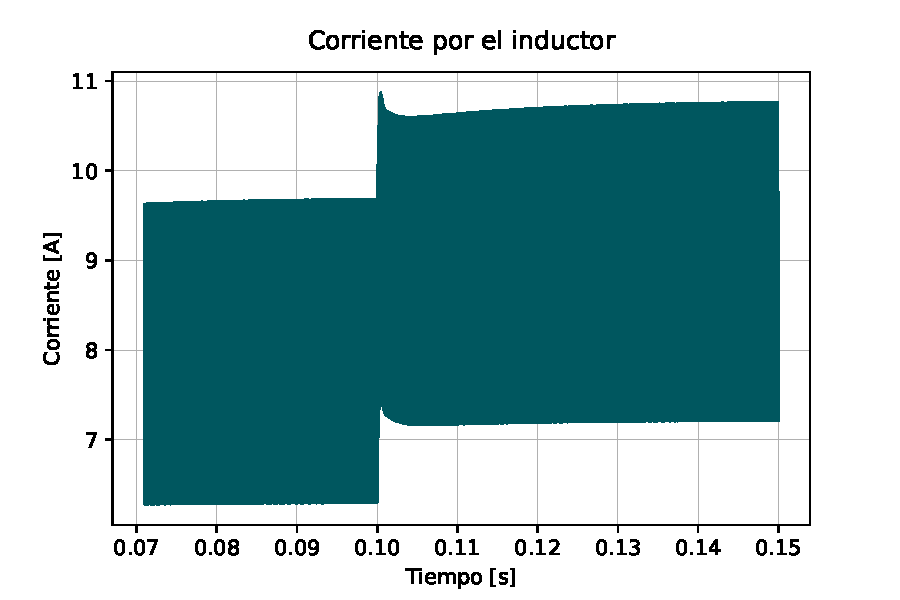
\includegraphics[width=0.45\textwidth]{Imágenes/Diseño del control/Simulación del lazo de corriente/Corriente por el inductor.pdf}}
  \hspace{3.5mm}
  \subfloat[Corriente por el inductor filtrada.]{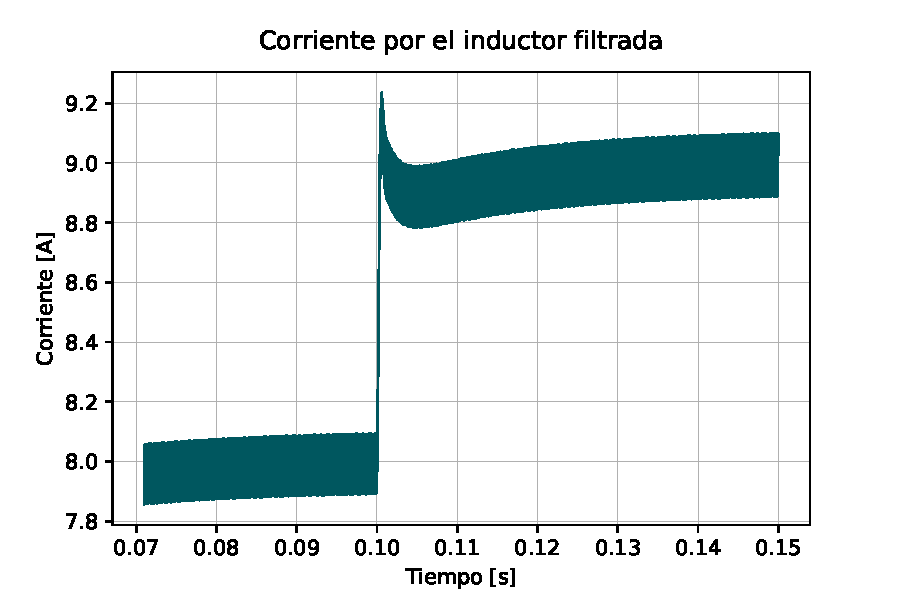
\includegraphics[width=0.45\textwidth]{Imágenes/Diseño del control/Simulación del lazo de corriente/Corriente por el inductor filtrada.pdf}}
  \hspace{3.5mm}
  \subfloat[Tensión en la salida.]{\includegraphics[width=0.45\textwidth]{Imágenes/Diseño del control/Simulación del lazo de corriente/Tensión en la salida.pdf}}
  \caption{Formas de onda obtenidas en la simulación del lazo de control de corriente.}
  \label{formas-onda-lazo-corriente}
\end{figure}

\begin{figure}[hbt!]
  \centering
  \subfloat[Corriente por el inductor en detalle.]{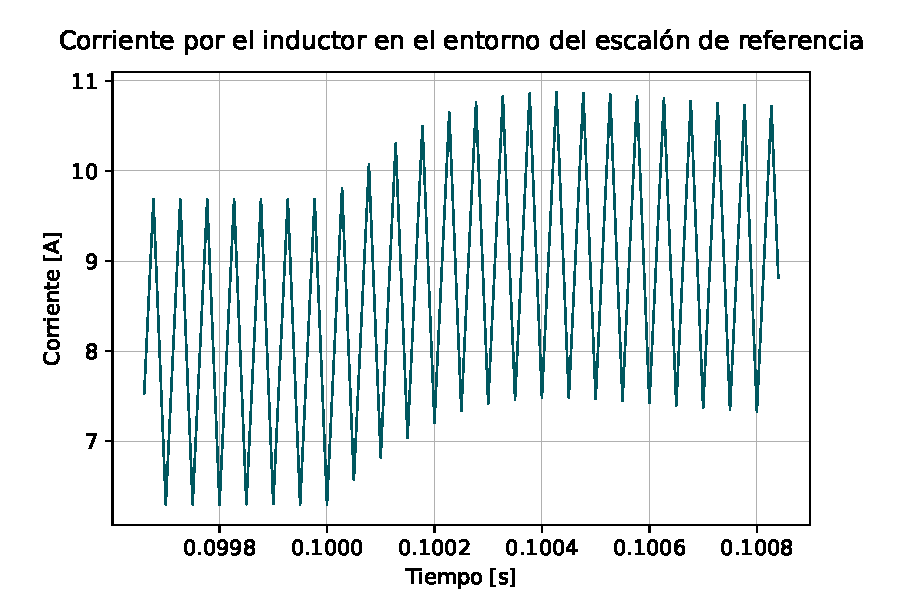
\includegraphics[width=0.45\textwidth]{Imágenes/Diseño del control/Simulación del lazo de corriente/Corriente por el inductor en entorno.pdf}}    
  \hspace{3.5mm}
  \subfloat[Corriente por el inductor filtrada en detalle.]{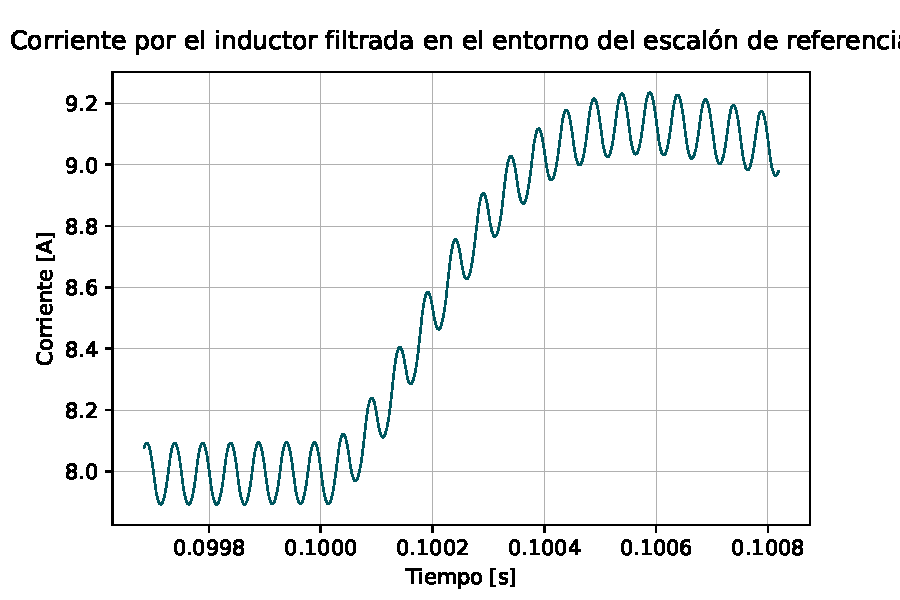
\includegraphics[width=0.45\textwidth]{Imágenes/Diseño del control/Simulación del lazo de corriente/Corriente por el inductor filtrada en entorno.pdf}}
  \hspace{3.5mm}
  \caption{Corriente del inductor alrededor del entorno del escalón unitario de corriente.}
  \label{formas-onda-filtradas-lazo-corriente}
\end{figure}

\subsection{Diseño del lazo externo de tensión}

Para el diseño del lazo de control de tensión y poder controlar la tensión de salida del convertidor, se implementa la estrategia de control que se muestra en la Figura \ref{lazo-tension}

\begin{figure}[hbt!]
  \centering
  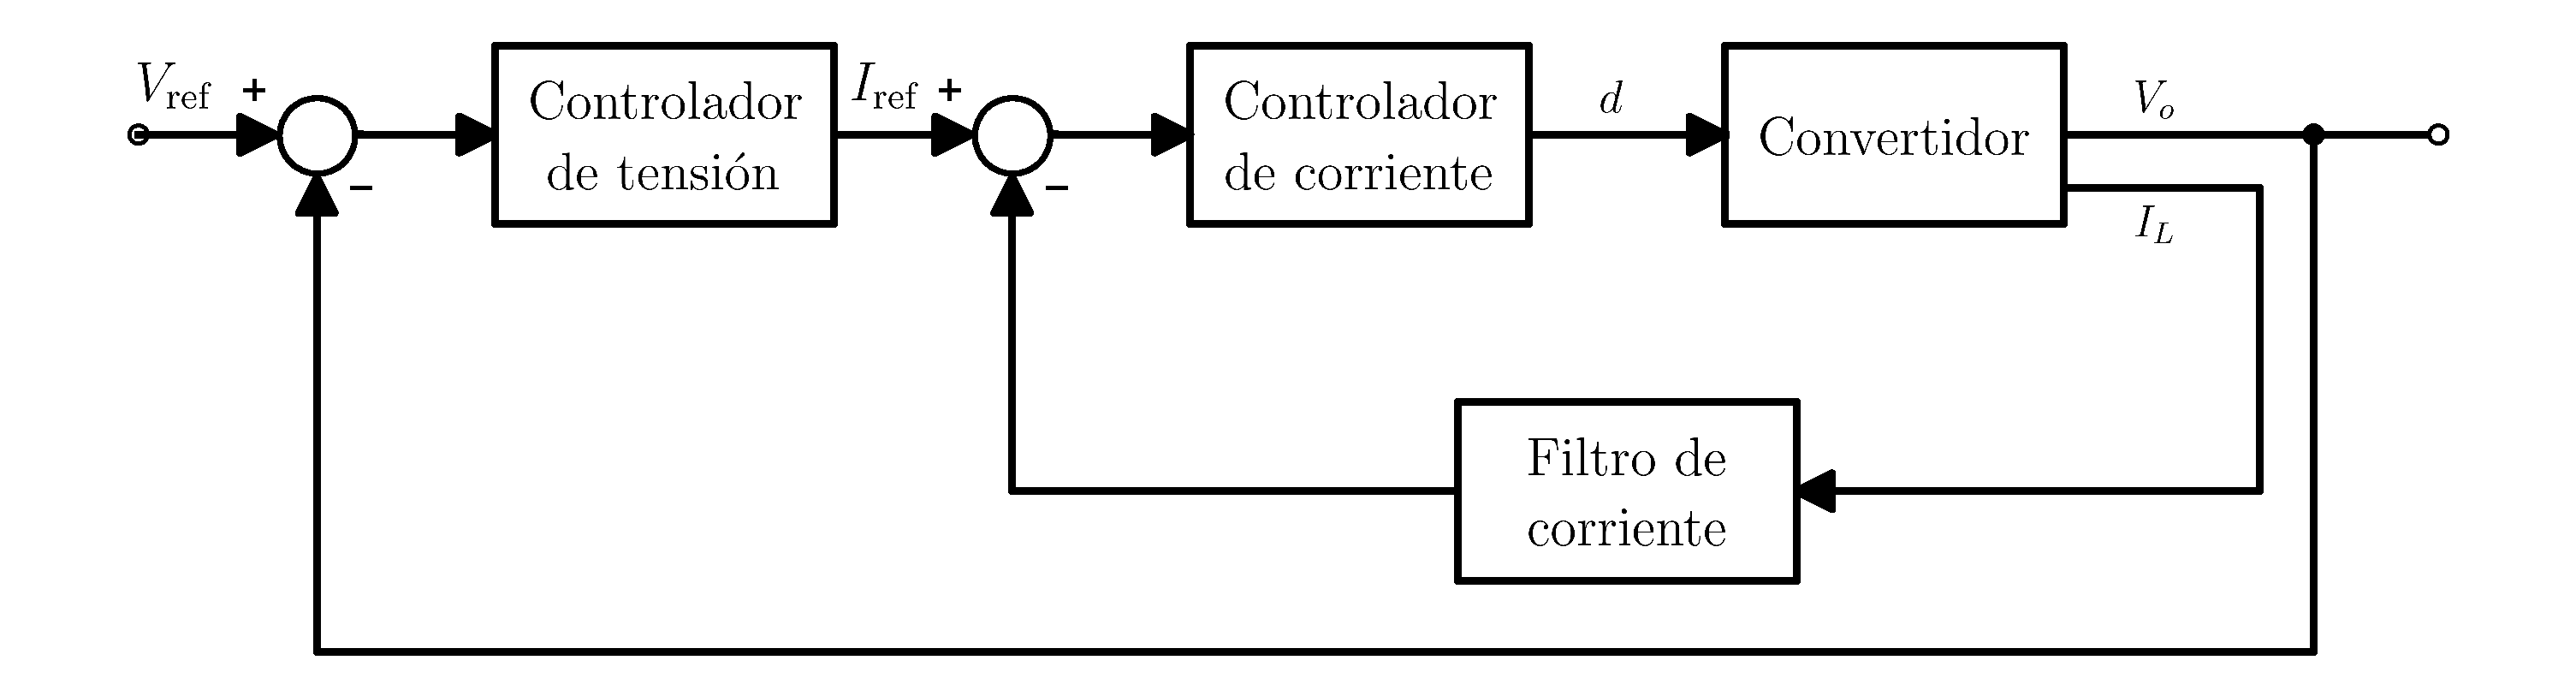
\includegraphics[width=0.80\columnwidth]{Imágenes/Diseño del control/Lazo de control de tensión.pdf}
  \caption{Ilustración del lazo de control de tensión.}
  \label{lazo-tension}
\end{figure} 

Como se puede observar, el lazo de corriente queda anidado dentro del de tensión y es visto como parte de la planta a controlar por este. Por lo tanto, es necesario realizar una expansión del modelo del sistema que incluya al lazo de control de corriente. Este debe incluir al convertidor, al lazo interno de corriente, y a su filtro correspondiente. Desarrollando mediante modelos de estados al controlador PI de corriente y a su filtro se obtienen las ecuaciones en diferencias correspondientes:

\begin{equation*}
  \begin{split}
    & x_1\left[n+1\right] = I_{\mathrm{ref}} - x_2\left[n\right]
    \\
    & x_2\left[n+1\right] = 0.0150796 \, i_L\left[n\right] + 0.98492 \, x_2\left[n\right]
  \end{split}
  \label{ecuaciones-extra}
\end{equation*}

Reemplazando,

\begin{equation*}
  d\left[n\right] = \left( I_{\mathrm{ref}} - x_2\left[n\right] \right) \, K_p + K_i \, T_s \, x_1\left[n\right]
\end{equation*}

Y sustituyendo con los valores correspondientes al controlador PI de corriente:

\begin{equation*}
  d\left[n\right] = 0.02 \, I_{\mathrm{ref}} -  0.02\, x_2\left[n\right] + 17.04 \times 10^{-6} \, x_1\left[n\right]
  \label{ecuacion-extra}
\end{equation*}

Expresando las ecuaciones diferenciales del modelo linealizado del convertidor dados por las \mbox{Ecuaciones \ref{sistema-modelo-lineal}} en ecuaciones en diferencias considerando un tiempo de muestro de \SI{1.42}{\micro\second} y el punto de trabajo establecido anteriormente, se obtiene:

\begin{equation*}
  \begin{split}
    &i_L \left[n+1\right] = i_L\left[n\right] - 0.00355 \, v_o\left[n\right] + 0.355 \, d\left[n\right]
    \\
    & v_o\left[n+1\right] = 0.00323 i_L\left[n\right] + 0.99996 \, v_o\left[n\right] - 0.00430 d \left[n\right]
  \end{split}
  \label{ecuaciones-originales-expansion}
\end{equation*}

Luego, expandiendo el sistema con las Ecuaciones \ref{ecuaciones-extra}, \ref{ecuacion-extra} y \ref{ecuaciones-originales-expansion}:

\begin{equation*}
  \begin{split}
    &i_L \left[n+1\right] = i_L\left[n\right] - 0.00355 \, v_o\left[n\right] + 0.355 \, \left[ 0.02 \, I_{\mathrm{ref}} -  0.02\, x_2\left[n\right] + 17.04 \times 10^{-6} \, x_1\left[n\right] \right]
    \\
    & v_o\left[n+1\right] = 0.00323 i_L\left[n\right] + 0.99996 \, v_o\left[n\right] - 0.00430 \left[ 0.02 \, I_{\mathrm{ref}} -  0.02\, x_2\left[n\right] + 17.04 \times 10^{-6} \, x_1\left[n\right] \right]
    \\
    & x_1\left[n+1\right] = I_{\mathrm{ref}} - x_2\left[n\right]
    \\
    & x_2\left[n+1\right] = 0.0150796 \, i_L\left[n\right] + 0.98492 \, x_2\left[n\right]
  \end{split}
\end{equation*}

Distribuyendo términos y generando una representación matricial:

\begin{align*}
  \boxed{
  \begin{bmatrix}
    i_L\left[n+1\right]\\
    v_o\left[n+1\right]\\  
    x_1\left[n+1\right]\\  
    x_2\left[n+1\right]\\  
  \end{bmatrix}
  =
  \begin{bmatrix}
    1 & -0.00355 & 6.0492 \times 10^{-6} & -7.1 \times 10^{-3}\\
    0.99996 & 3.23 \times 10^{-3} & -73.272 \times 10^{-9} & 86 \times 10^{-6}\\
    0 & 0 & 0 & -1 \\
    15.0796 \times 10^{-3} & 0 & 0 & 0.98492 \\
  \end{bmatrix}
  \,
  \begin{bmatrix}
    i_L\left[n\right]\\
    v_o\left[n\right]\\  
    x_1\left[n\right]\\  
    x_2\left[n\right]\\  
  \end{bmatrix}
  +
  \begin{bmatrix}
    7.1 \times 10^{-3}\\
    86 \times 10^{-6}\\  
    1\\  
    0\\  
  \end{bmatrix}
  \,
  I_{\mathrm{ref}}
  }
\end{align*}

Este sistema discreto expandido representa a la planta a lazo cerrado de corriente. Una cuestión crítica a tener en cuenta a la hora de empezar a diseñar el lazo de tensión es que su dinámica debe ser aproximadamente un orden de magnitud más lenta que la del lazo de corriente, para que esta pueda seguir su referencia de forma adecuada y sin provocar un comportamiento oscilatorio.

La sintonía del controlador de tensión fue realizada con el mismo método que el utilizado para sintonizar el PI de corriente, mediante una aproximación lineal y ajustes progresivos basados en la respuesta temporal observada. El siguiente controlador proporcional-integral de tensión fue obtenido:

\begin{equation*}
  \mathrm{PI}_U = K_{p_U} + \frac{K_{i_U} \, T_s}{z-1} 
\end{equation*}

\begin{equation*}
  \boxed{\mathrm{PI}_U = 0.2 + \frac{15 \cdot \, 1.6 \times 10^{-6}}{z-1}}
\end{equation*}

Lo que implica $K_{p_U} = 0.2$ y $K_{i_U} = 15$. En la Figura \ref{simulacion-modelo-real-tension} se ilustra el diagrama en bloques armado para la simulación del modelo real. En el lazo de control se puede observar el control de la tensión junto con el control de corriente anidado, y el muestreo de las variables de estado del convertidor electrónico. 

\begin{figure}[hbt!]
  \centering
  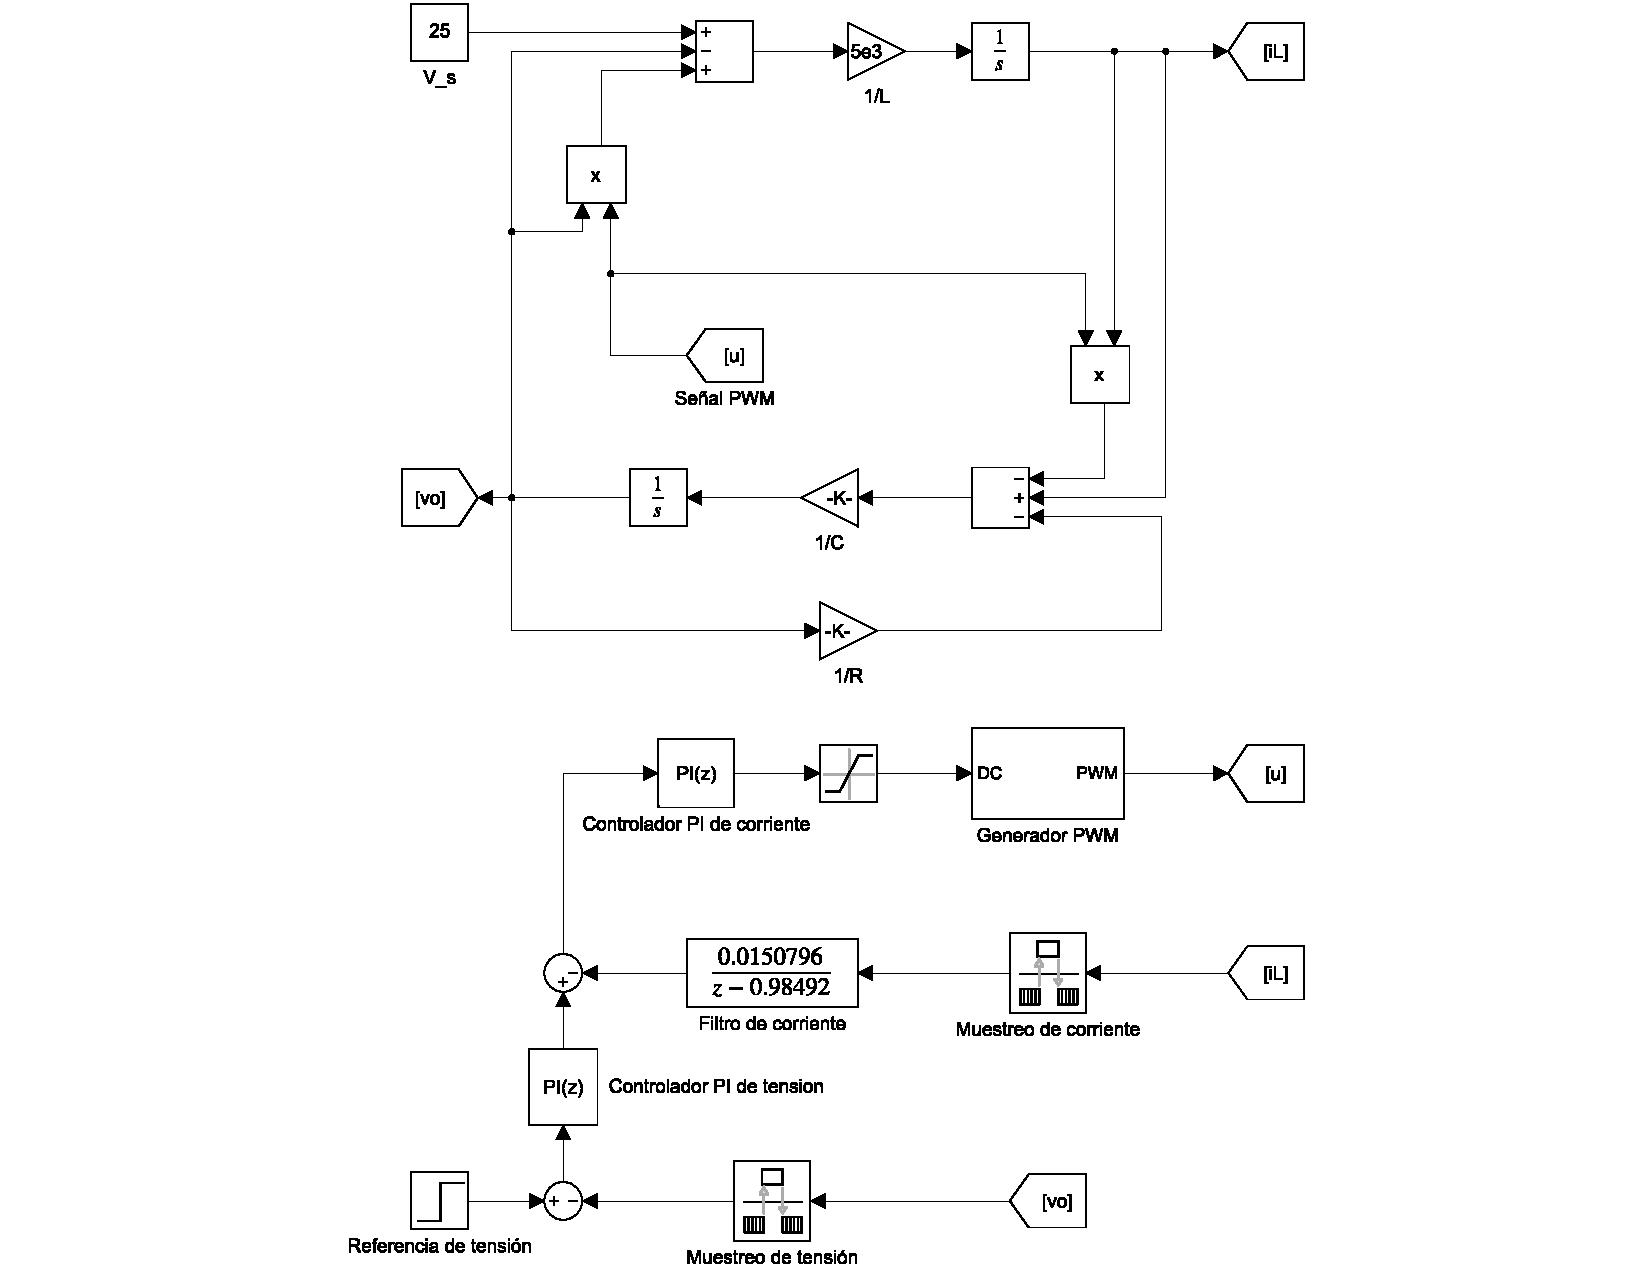
\includegraphics[width=0.75\columnwidth]{Imágenes/Diseño del control/Simulación del lazo de tensión/Simulación real del lazo de tensión.pdf}
  \caption{Simulación real del lazo de control de tensión.}
  \label{simulacion-modelo-real-tension}
\end{figure} 

La simulación realizada para este sistema es similar a la del lazo de corriente. Se inyectó nuevamente un escalón a la referencia de tensión que varía de \SI{50}{\volt} a \SI{55}{\volt} a los \SI{0.25}{\second}, y se observan las mismas formas de onda graficadas anteriormente. En el escalón de referencia no se discierne un sobrepico de tensión en la salida, y nuevamente utilizando las herramientas de Simulink\textsuperscript\textregistered \hspace{0.6pt} se mide el tiempo de establecimiento al 2\%, el cual resulta ser de aproximadamente \SI{70}{\milli\second}.

\begin{figure}[hbt!]
  \centering
  \subfloat[Referencia de tensión.]{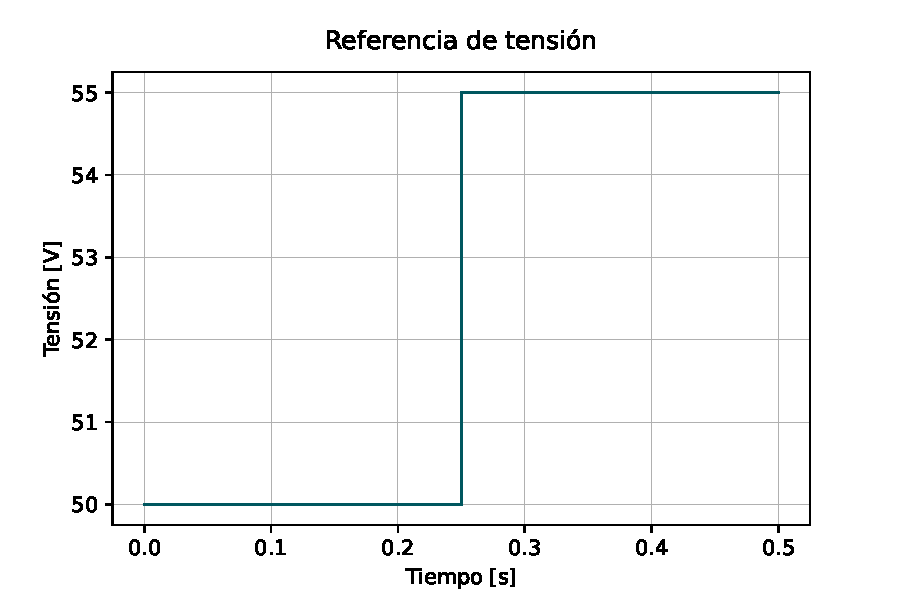
\includegraphics[width=0.45\textwidth]{Imágenes/Diseño del control/Simulación del lazo de tensión/Referencia de tensión.pdf}}    
  \hspace{3.5mm}
  \subfloat[Tensión en la salida.]{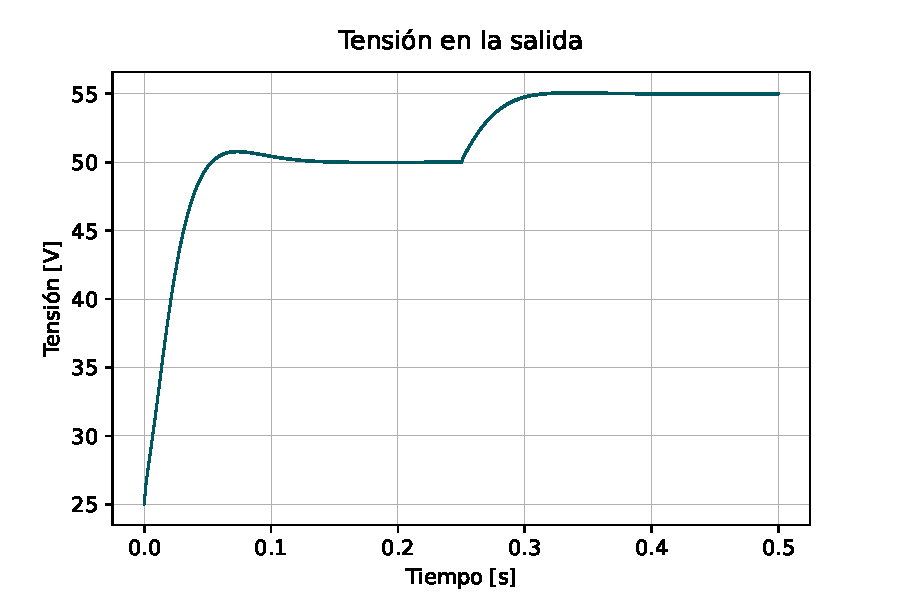
\includegraphics[width=0.45\textwidth]{Imágenes/Diseño del control/Simulación del lazo de tensión/Tensión en la salida.pdf}}
  \hspace{3.5mm}
  \subfloat[Corriente por el inductor filtrada.]{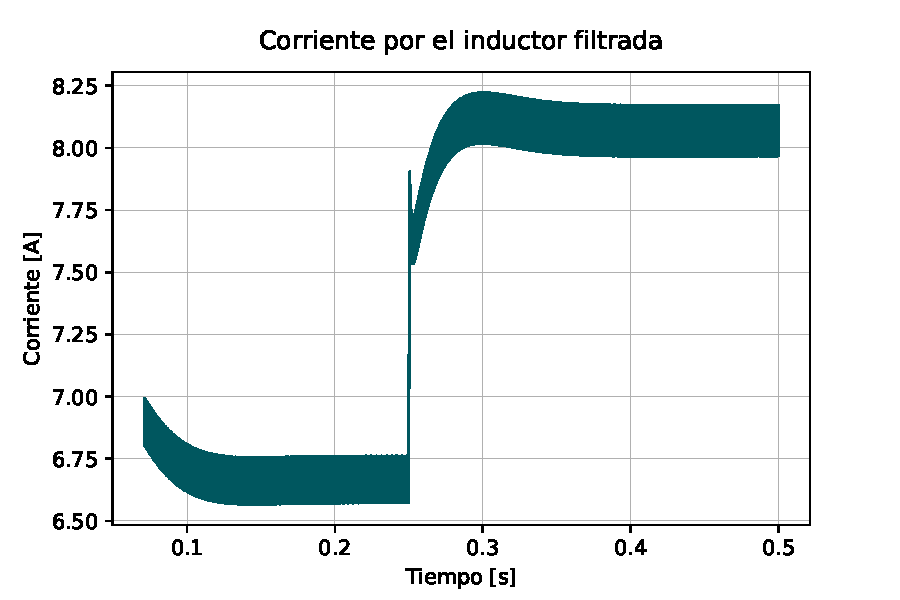
\includegraphics[width=0.45\textwidth]{Imágenes/Diseño del control/Simulación del lazo de tensión/Corriente por el inductor filtrada.pdf}}
  \hspace{3.5mm}
  \subfloat[Corriente por el inductor.]{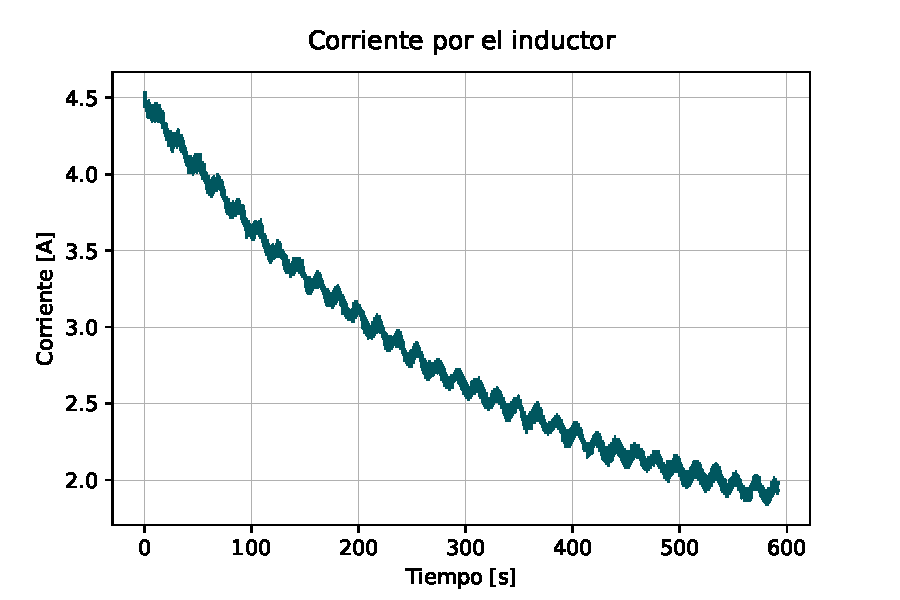
\includegraphics[width=0.45\textwidth]{Imágenes/Diseño del control/Simulación del lazo de tensión/Corriente por el inductor.pdf}}
  \caption{Formas de onda obtenidas en la simulación del lazo de control de tensión.}
  \label{formas-onda-lazo-tension}
\end{figure}

\subsubsection{Variación de la resistencia de carga}

La última prueba en Simulink\textsuperscript\textregistered \hspace{0.6pt} se realiza modificando la carga conectada al convertidor elevador a lazo cerrado de tensión. Esta simulación se aproxima mejor a una situación real en la cual la demanda de la carga presenta una variación mientras está conectada al sistema.

Esta simulación consiste en hacer variar la resistencia de carga de un valor incial de \SI{15}{\ohm} a un valor de \SI{12}{\ohm} en t = \SI{0.25}{\second}. En la Figura \ref{var-carga-simulink} puede observarse la modificación realizada al modelo para poder realizar esta prueba.

\begin{figure}[hbt!]
  \centering
  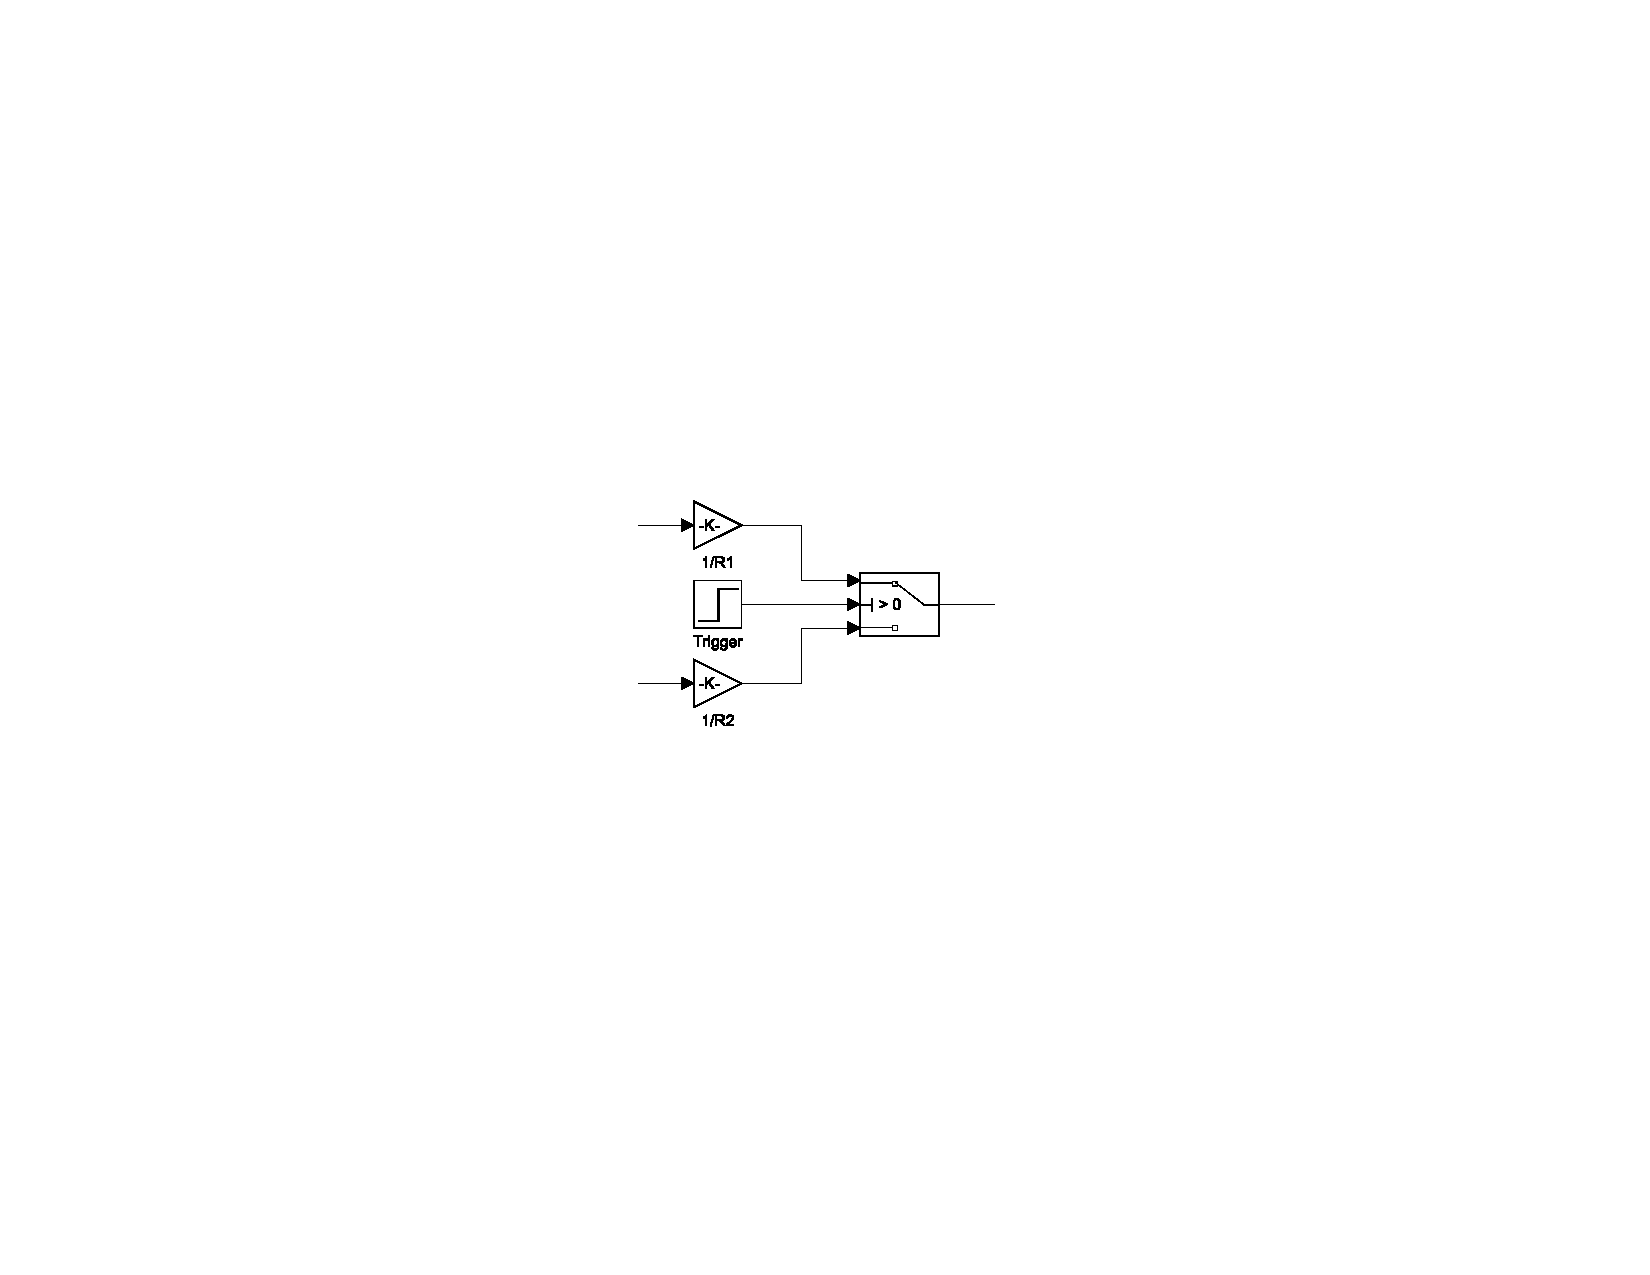
\includegraphics[width=0.35\columnwidth]{Imágenes/Diseño del control/Variación de parámetros de carga/Variación de resistencia de carga/Estructura en Simulink.pdf}
  \caption{Bloques reemplazados para simular una variación de carga.}
  \label{var-carga-simulink}
\end{figure} 

Simulando por un tiempo de \SI{0.5}{\second} a la variación de la resistencia de carga, la tensión que cae en ella, la corriente de por el inductor filtrada, y la acción de control, se obtienen la Figura \ref{formas-onda-var-carga}. Aquí se puede observar la adecuada respuesta del sistema de control ante este tipo de perturbaciones sin presentar sobrepicos y con un comportamiento suave y lo suficientemente rápido para volver a la tensión establecida a partir de la referencia elegida.

\begin{figure}[hbt!]
  \centering
  \subfloat[Variación de la resistencia.]{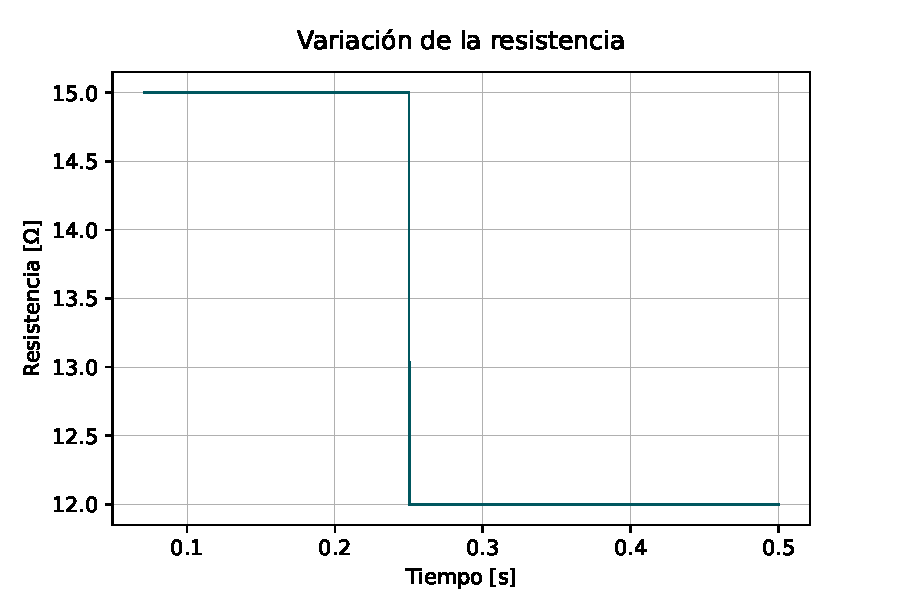
\includegraphics[width=0.45\textwidth]{Imágenes/Diseño del control/Variación de parámetros de carga/Variación de resistencia de carga/Variación de la resistencia.pdf}}    
  \hspace{3.5mm}
  \subfloat[Tensión en la salida.]{\includegraphics[width=0.45\textwidth]{Imágenes/Diseño del control/Variación de parámetros de carga/Variación de resistencia de carga/Tensión en la salida.pdf}}
  \hspace{3.5mm}
  \subfloat[Corriente por el inductor filtrada.]{\includegraphics[width=0.45\textwidth]{Imágenes/Diseño del control/Variación de parámetros de carga/Variación de resistencia de carga/Corriente por el inductor filtrada.pdf}}
  \hspace{3.5mm}
  \subfloat[Acción de control.]{\includegraphics[width=0.45\textwidth]{Imágenes/Diseño del control/Variación de parámetros de carga/Variación de resistencia de carga/Acción de control.pdf}}
  \caption{Formas de onda obtenidas en la simulación de una variación de la resistencia de carga.}
  \label{formas-onda-var-carga}
\end{figure}

\section{Resumen}

En este capítulo se ha expuesto el proceso de diseño del sistema de control a implementar, a través del desarrollo de las ecuaciones matemáticas que rigen a sus componentes (el filtro y los controladores), así como las que describen a un modelo del sistema lo suficientemente sencillo para poder utilizar las herramientas convencionales de análisis. 

Además se incluyeron simulaciones en cada etapa del proceso para corroborar el correcto funcionamiento de la acción de control provista por el sistema diseñado, y por último se realizaron una serie de simulaciones con el propósito de emular eventos que puedan ocurrir en el sistema real, para observar el comportamiento satisfactorio del sistema en el lazo cerrado de control creado.

En el próximo capítulo se muestra la programación de este sistema en el circuito de desarrollo utilizado para este trabajo, una FPGA con el lenguaje VHDL, y se realizan nuevas simulaciones en el entorno de este lenguaje HDL para confirmar su correcta implementación. 

\newpage

\chapter{Implementación de la etapa de control}
\label{implementacion-control}

\section{Introducción}

En este capítulo se sintetiza e implementa la estrategia de control diseñada en el capítulo anterior. Debido a las características del lenguaje de programación a utilizar, los componentes del lazo de control deben ser programados individualmente, para después ser ensamblados en el sistema de control diseñado. Debido a esta propiedad de VHDL, además de la programación de cada componente, se realiza una simulación o \emph{test bench} para corroborar su correcto funcionamiento. Las herramientas utilizadas aquí fueron el entorno de desarrollo Xilinx ISE\textsuperscript\textregistered \hspace{0.6pt} y los simuladores de código HDL ISim\textsuperscript\textregistered \hspace{0.6pt} y ModelSim\textsuperscript\textregistered \hspace{0.6pt}, los cuales fueron descritos en el Capítulo \ref{cap-fpga} Sección \ref{desarrollo-fpga}.

\section{Placa de desarrollo a utilizar}

\begin{wrapfigure}{r}{0.42\textwidth}
    \vspace{-10pt}
    \begin{center}
      \includegraphics[width=0.41\textwidth]{Imágenes/Nexys 3.png}
    \end{center}
    \caption{Placa de desarrollo Nexys 3.}
    \label{nexys3}
  \end{wrapfigure}

En el Capítulo \ref{cap-fpga}, Sección \ref{subseccion-nexys-3}, fue presentada la placa de desarrollo Nexys 3, la cual posee un FPGA Spartan-6. Esta placa es la utilizada para implementar el algoritmo de control que se detallará a lo largo de este capítulo, debido a su gran cantidad de recursos lógicos y amplia cantidad de elementos I/O (botones, switches, LEDs, etc.).

Esta placa presenta \emph{slices} específicamente diseñados para aplicaciones de procesamiento de señales (llamados \mbox{\emph{DSP slices}}), los que permiten un cálculo de punto fijo con gran resolución, funcionalidad necesaria para sintetizar los controladores y filtros mostrados en esta sección.

Para la programación de la Nexys 3 es necesario utilizar el entorno de desarrollo de Xilinx\textsuperscript\textregistered \hspace{0.6pt}, el cual posee varias herramientas que permitirán verificar el correcto funcionamiento de cada modelo programado y visualizar el interconexionado de cada bloque que conforma el sistema de control implementado. 

\section{Implementación de la etapa de control}

\subsection{Conversor analógico-digital}

La primer pieza del lazo de control programada fue el controlador de los conversores analógico-digitales. Previo a esta tarea fue necesario comprender el protocolo de comunicación del \emph{Pmod AD1}, el cual está compuesto por dos ADC \emph{AD7476A} de Analog Devices. El protocolo utilizado por estos conversores es \emph{SPI-like} con una señal de \emph{Chip Select} ($\overline{\mbox{CS}}$), con la única diferencia de que ambas líneas de datos (\emph{MOSI} y \emph{MISO}) son diseñadas para operar únicamente como salidas, y por lo tanto ambas son definidas como líneas de datos \emph{Master-In-Slave-Out}.

Los ADCs poseen una resolución de 12 bits, con una frecuencia de muestreo máxima de 1MS/s y un filtro antialiasing \cite{ad7476a}. Ambos conversores transforman una señal que va de 0 a $\mathrm{V_{DD}}$, en un valor digital con un rango de 0 a 4095. En la Figura \ref{diagramas-adc} pueden observarse los diagramas circuitales del Pmod AD1 y de los AD7476A.

\begin{figure}[hbt!]
    \centering
    \subfloat[Pmod AD1.]{\includegraphics[width=0.3\textwidth]{Imágenes/Conversor analógico-digital/Pmod AD1.pdf}}    
    \hspace{10mm}
    \subfloat[AD7476A.]{\includegraphics[width=0.27\textwidth]{Imágenes/Conversor analógico-digital/AD7476A.pdf}}
    \caption{Diagramas de los circuitos del Pmod y ADC.}
    \label{diagramas-adc}
\end{figure}

El principio de funcionamiento de los conversores consta del $\overline{\mbox{CS}}$ y un reloj en serie SCLK. Cuando se produce un flanco en SCLK y $\overline{\mbox{CS}}$ está bajo, los conversores empiezan a muestrear. En total, cada ADC produce 16 bits, en donde los cuatro primeros bits son cero, y los restantes 12 bits son la muestra con el bit más significativo primero. En la Figura \ref{adc-timing} se observa el diagrama de tiempos del conversor.

\begin{figure}[hbt!]
    \centering
    \includegraphics[width=0.85\columnwidth]{Imágenes/Conversor analógico-digital/Diagrama de tiempos del AD7476A.pdf}
    \caption{Diagrama de tiempos del AD7476A.}
    \label{adc-timing}
\end{figure} 

Para poder utilizar ambos conversores se implementó un controlador en VHDL a partir de una máquina de tres estados:

\begin{enumerate}
    \item En el estado \texttt{shift} se captan las muestras de ambos ADCs y se los almacena en registros auxiliares de 16 bits.
    \item En el estado \texttt{sync} se copian los 12 bits de ambas muestras a los puertos de salida correspondientes de cada conversor.
    \item Por último, en el estado \texttt{idle} el controlador permanece inactivo, lo cual es necesario entre conversiones.
\end{enumerate}

En la Figura \ref{adc-controller} puede observarse el \emph{test bench} realizado para el controlador con el software ModelSim\textsuperscript\textregistered.

\begin{figure}[hbt!]
    \centering
    \includegraphics[width=0.85\columnwidth]{Imágenes/Conversor analógico-digital/Test bench.pdf}
    \caption{Simulación realizada del controlador de los conversores.}
    \label{adc-controller}
\end{figure} 

En esta simulación, \texttt{start} se pone en alto, y cuando el controlador recibe un flanco ascendente de \texttt{sclk}, \texttt{cs} se pone en bajo. Esto significa que la conversión comienza a efectuarse. Luego de iniciar el muestreo, se reciben en los siguientes ocho flancos ascendentes del reloj todos ceros en \texttt{sdata\_1}, y luego el patrón que puede observarse (un uno, un cero, otro uno, un cero más, y luego todos unos, en ese orden). Finalmente, después de 16 ciclos de \texttt{sclk}, los datos se sincronizan a través de la máquina de estados en un vector de 12 bits llamado \texttt{data\_1}, en el cual se descartan los primeros 4 ceros.

En este controlador, \texttt{sclk} es un reloj de frecuencia \SI{12.5}{\mega\hertz}, mientras que la frecuencia de muestreo (lo que sería \texttt{start}) es de \SI{625}{\kilo\hertz}. 

\subsection{Filtro digital}

Una vez muestreada la corriente, es importante que el lazo interno de corriente reciba un valor medio para que su dinámica resulte suave y no se produzcan exabruptos que puedan poner en peligro al sistema. Por lo tanto, un filtro es diseñado para atenuar el \emph{ripple} de la corriente, resultado de la conmutación de las llaves del convertidor como fue mencionado en capítulos anteriores y puede observarse en la Figura \ref{formas-onda-elevador}b. Por eso mismo, se implementa un filtro pasabajos digital de primer orden, con frecuencia de corte $f_c$ de 1.5kHz. La razón de esta elección fue mencionada en el Capítulo \ref{diseno-control}, Sección \ref{diseno-filtro-corriente}. La Ecuación \ref{filtro-corriente-discretizado} representa a la transferencia discreta del filtro a implementar. Desarrollando la función de transferencia:

\begin{equation*}
    z \, Y(z) - 0.98492 \, Y(z) = 0.0150796 \, X(z)
\end{equation*}

Y antitransformando:

\begin{equation}
    y[n+1] - 0.98492 \, y[n] = 0.0150796 \, x[n]
    \label{filtro-anticausal}
\end{equation}

Esta ecuación en diferencias es \emph{anticausal}, es decir, el término $y[n+1]$ representa una muestra de la salida en un tiempo futuro, lo cual físicamente no es posible de sintetizar. Por lo tanto, para implementar la Ecuación \ref{filtro-anticausal} es necesario aplicar un retardo unitario al sistema. Implementando el retardo y reordenardo, la expresión final es la siguiente:

\begin{equation}
    \boxed{y[n] = 0.0150796 \, x[n-1] + 0.98492 \, y[n-1]}
\end{equation}

La implementación del filtro puede ser optimizada para que se utilice un único \emph{delay} para ambas entrada y salida. Su síntesis en Simulink\textsuperscript\textregistered \hspace{0.6pt} puede observarse en la Figura \ref{estructura-filtro}.

\begin{figure}[hbt!]
    \centering
    \includegraphics[width=0.85\columnwidth]{Imágenes/Filtro digital/Estructura en Simulink.pdf}    
    \caption{Implementación del filtro en Simulink\textsuperscript\textregistered.}
    \label{estructura-filtro}
\end{figure}

Con $k_o = 0.0150796$ y $k_1 = 0.98492$. Debido a la resolución necesaria para representar estos coeficientes, se eligió una síntesis a código HDL con representación en punto fijo de 32 bits de longitud de palabra, con 16 bits para representar la fracción.

Generado el código de VHDL, se realiza nuevamente otro \emph{test bench} para probar su funcionamiento. Para esta simulación se inyecta una onda triangular con amplitud unitaria de 20kHz montada sobre una señal continua de valor 1, de forma de emular el comportamiento de la corriente del convertidor. El resultado puede verse en la Figura \ref{simulacion-filtro}, en el cual se observa un transitorio y luego el correcto filtrado del \emph{ripple} de la entrada.

\begin{figure}[hbt!]
    \centering
    \includegraphics[width=0.85\columnwidth]{Imágenes/Filtro digital/Simulación en ModelSim.pdf}    
    \caption{Simulación realizada del controlador de los conversores.}
    \label{simulacion-filtro}
\end{figure} 

\subsection{Controlador proporcional-integral}
\label{implementacion-pid}

La programación en VHDL de los controladores PI fue realizada con el mismo procedimiento que el de los filtros digitales. El diagrama en bloques creado en Simulink\textsuperscript\textregistered\hspace{0.05pt} es el de la Figura \ref{estructura-pi}. En este diagrama pueden visualizarse dos saturaciones: la primera, llamada \texttt{saturation}, evita que la acción de control calculada por el PI exceda los límites inferiores y superiores impuestos por él; mientras que \texttt{clamping} cumple el rol de sistema \emph{anti-windup} (explicado en el Capítulo \ref{diseno-control}, Sección \ref{diseno-controladores-pid}). El tipo de datos para la representación de los parámetros diseñados fue de punto fijo de 32 bits de longitud de palabra, con 16 bits para la fracción.

\begin{figure}[hbt!]
    \centering
    \includegraphics[width=0.70\columnwidth]{Imágenes/Controlador proporcional-integral/Estructura en Simulink.pdf}    
    \caption{Implementación del controlador PI en Simulink\textsuperscript\textregistered.}
    \label{estructura-pi}
\end{figure}

Como los mecanismos de ambos controladores PI son iguales, se programa una única simulación. El \emph{test bench} realizado para los controladores proporcional-integral consiste en la prueba del correcto funcionamiento del clamping, utilizando un estímulo constante de valor unitario positivo hasta el valor fijado (240 en entero o 0F0 en hexadecimal), seguido de un breve período sin excitación, y finalmente una excitación con un valor entero negativo para observar como llega a cero. Tal simulación se muestra en la Figura \ref{simulacion-pi}. Se observa el correcto funcionamiento del controlador en las tres etapas, ya que una entrada constante se traduce a una rampa gracias al integrador, luego se observa la saturación debido al clamping y su mantenimiento a través de la excitación nula, y por último su rampa con pendiente negativa hasta el cero debido a una señal de error negativa.

\begin{figure}[hbt!]
    \centering
    \includegraphics[width=0.85\columnwidth]{Imágenes/Controlador proporcional-integral/Simulacion en ModelSim.pdf}    
    \caption{Simulación realizada del controlador proporcional-integral.}
    \label{simulacion-pi}
\end{figure} 

Para cada controlador proporcional-integral se implementó un \emph{reset} que permite la habilitación de su parte integral. 

\subsection{Referencia}

Para poder establecer un valor de tensión o corriente que el sistema de control tenga que seguir, un bloque de referencia fue implementado. Este bloque consiste en dos señales de referencia: 

\begin{itemize}
    \item La señal de referencia de tensión, la cual se encuentra inicializada en \SI{10}{\volt} y puede aumentarse o reducirse en escalones de \SI{1}{\volt}. Esta señal puede ser modificada sólo si el lazo externo de control de tensión se encuentra habilitado mediante el \emph{reset} mencionado anteriormente.
    \item La señal de referencia de corriente, la cual es inicializada en \SI{0}{\ampere} y sus escalones son de \SI{0.125}{\ampere}. Esta señal puede ser modificada sólo si el lazo de tensión se encuentra deshabilitado.
\end{itemize}

Ambas señales de referencia son representadas con punto fijo de 32 bits de palabra, con 16 bits para la fracción, al igual que los controladores PI.

\subsection{Controlador PWM}

El generador de la onda modulada por ancho de pulsos hace de vínculo entre la acción de control y el convertidor. Este bloque recibe como entrada un ciclo de trabajo provisto por el controlador proporcional-integral, y comparándolo con un contador, lo transforma en una señal de ancho de pulso modulado (PWM). Este bloque posee como salidas la señal PWM y su complemento para accionar ambas llaves del convertidor.

El controlador fue programado completamente en VHDL y recibe un ciclo de trabajo con resolución de 12 bits (al igual que la resolución de las muestras de los conversores analógico-digitales), generando una onda PWM correspondiente con una frecuencia de 20kHz a partir de un contador y un comparador. En la Figura \ref{simulacion-pwm} se ingresa al controlador con el valor decimal 2047, que genera una onda de ancho de pulso modulado con un ciclo de trabajo del 50\%, y también se puede corroborar que su período es de \SI{50}{\micro\second}.

\begin{figure}[hbt!]
    \centering
    \includegraphics[width=0.85\columnwidth]{Imágenes/Controlador PWM/Simulación en ModelSim.pdf}    
    \caption{Simulación realizada del controlador PWM.}
    \label{simulacion-pwm}
\end{figure} 

\section{Implementación de módulos auxiliares}

\subsection{Display de siete segmentos}

Para la visualización de las mediciones y referencias de corriente de entrada y tensión de salida se utilizaron los cinco display de siete segmentos que posee la placa de desarrollo Nexys 3. La selección de la variable a representar en los display se selecciona mediante un registro el cual es manejado a través de un par de botones.

\subsection{Botones de selección y referencia}

Para el sistema de control, cuatro botones fueron utilizados. Dos de ellos permiten el control de los display siete segmentos, como fue mencionado anteriormente, y el otro par permiten el aumento o reducción del valor de referencia seleccionado. Para la implementación de los botones fue necesario programar un componente antirrebote de aproximadamente 100 milisegundos, el cual fue luego instanciado cuatro veces (una para cada botón).

\subsection{Llaves de habilitación}

Por motivos de seguridad, se recurrió al uso de tres llaves de las ocho que posee la placa de desarrollo. Estas consisten en la habilitación o deshabilitación de un componente en específico en el caso de que surja un comportamiento que pueda poner en peligro al sistema, o si se quisiera realizar una habilitación secuencial de los componentes para un ensayo más controlado.

Las llaves utilizadas controlan los siguientes componentes:

\begin{enumerate}
    \item El bloque generador de la señal PWM. Si esta llave es habilitada, la señal PWM y su complemento son llevadas a un nivel bajo.
    \item El componente integrador del controlador PI de corriente.  
    \item El lazo de control de tensión. Si se encuentra en alto, el integrador se desactiva, y la acción de control generada por el lazo externo se desconecta del lazo interno, el cual a su vez se conecta a una referencia con un valor establecido manualmente.
\end{enumerate}

\subsection{Comunicación UART}

Un transmisor UART (del inglés \emph{Universal Asynchronous Receiver-Transmitter}) fue programado en el FPGA para poder enviar las mediciones y acciones de control calculadas a una computadora. Debido a que este tipo de comunicación consiste en paquetes de 10 bits (dos bits de inicio y fin, y ocho de datos), se decidió implementar un transmisor que sea capaz de enviar en 64 bits de datos, divididos de la siguiente manera:

\begin{enumerate}
    \item 12 bits correspondientes a la medición de tensión de carga.
    \item 12 bits correspondientes a la medición de corriente de entrada.
    \item 12 bits correspondientes a la acción de control del lazo interno de corriente.
    \item 28 bits correspondientes a la acción de control del lazo externo de tensión.
\end{enumerate}

En la Figura \ref{uart} puede observarse el diagrama de tiempos de cada paquete correspondiente al protocolo de comunicación UART.

\begin{figure}[hbt!]
    \centering
    \includegraphics[width=0.65\columnwidth]{Imágenes/UART.pdf}
    \caption{Diagrama de tiempos del protocolo de comunicación UART.}
    \label{uart}
\end{figure} 

Ya que en este tipo de comunicación asincrónica no es posible recibir los datos en orden, se utilizaron otros 64 bits para indexar cada paquete de datos. La recepción y reordenamiento de los paquetes transmitidos por la Nexys 3 fue hecho en MATLAB\textsuperscript\textregistered. Para poder ordenar cada paquete, cuatro bits de datos fueron utilizados para un número en hexadecimal (de 0 a F), y los otros cuatro bits para los datos a transmitir. En total son transmitidos 160 bits a una tasa de 256000 baudios.

\section{Construcción del sistema de control}

Una vez programados todos los componentes, se realiza la interconexión entre ellos. Esto es logrado a través de la instanciación de cada modelo en un \emph{top-level file}, concepto detallado en el Capítulo \ref{cap-fpga}. El modelo resultante, al tratarse solamente de la vinculación entre cada componente, posee una arquitectura estructural, como fue explicado en la Sección \ref{vhdl-estruct}.

El sistema de control está compuesto por los componentes propios que permiten la medición de las variables, su filtrado, y el cálculo de la acción de control a partir de una referencia establecida por el usuario. Los módulos auxiliares generan la interfaz entre la placa de desarrollo y su operador, y posibilita la visualización de las variables y las referencias, así como la manipulación de estas últimas. En el caso de ser necesario, el operador también puede utilizar las tres llaves de seguridad programadas.

Con el lazo de control armado con todos sus componentes y sintetizado en Xilinx ISE\textsuperscript\textregistered\hspace{0.05pt}, se observa su diagrama RTL (del inglés \emph{register-transfer level}, lo cual equivale a un diagrama de bloques y señales para lenguajes HDL) creado por el entorno de desarrollo en la Figura \ref{rtl-lazo}.

\begin{figure}[hbt!]
    \centering
    \includegraphics[width=0.65\columnwidth]{Imágenes/Diagrama RTL del lazo de tensión.pdf}    
    \caption{Diagrama RTL del lazo de tensión.}
    \label{rtl-lazo}
\end{figure} 

\section{Resumen}

En este capítulo fue mostrada la implementación de los bloques del sistema de control diseñado. Para esto, fue necesario utilizar varias herramientas que permitieron su traducción a VHDL, la síntesis de este código generado, y finalmente la simulación y ensayo de cada componente para verificar su correcto funcionamiento. Para la representación de las señales calculadas en cada instanciación, se eligió un tipo de dato de punto fijo que permitió su cálculo con un bajo error, de manera de poder generar un ciclo de trabajo preciso que es alimentado al convertidor electrónico de potencia. 

\newpage

\chapter{Ensayos y resultados experimentales}

\section{Introducción}

Una vez implementado el sistema de control diseñado en la placa de desarrollo Nexys 3, se realizan una serie de ensayos para verificar su correcto funcionamiento. Estos ensayos fueron realizados en forma progresiva, en un principio probando sólamente el generador PWM junto con el ADC en un esquema lazo abierto. Luego de ir confirmando el correcto funcionamiento, se fueron agregando más componentes para finalmente realizar un ensayo con el lazo cerrado de tensión.

\section{Pruebas a lazo abierto}

Las primeras pruebas realizadas a lazo abierto consistieron en la utilización del controlador PWM para las señales de los transistores del convertidor CC-CC. Luego, se implementó al controlador del conversor analógico-digital para permitir la variación del ciclo de trabajo mediante un potenciómetro, cuyo valor era filtrado por el filtro diseñado e implementado a \SI{1.5}{\kilo\hertz}.

\section{Pruebas a lazo cerrado}

\subsection{Lazo de control de corriente}

El primer ensayo a lazo cerrado consistió en el control de la corriente por el inductor del convertidor CC-CC. En este sistema fueron utilizados los componentes ya probados anteriormente: el controlador PWM; el controlador del ADC; y el filtro de corriente de \SI{1.5}{\kilo\hertz}. Para poder cerrar el lazo, se incorporaron dos nuevos elementos: la referencia, para poder establecer un valor en el cual la corriente se establezca; y el controlador PI, para poder calcular la acción de control que permita seguir a la referencia.

Como medida de seguridad, se implementaron llaves que permiten habilitar o deshabilitar el integrador del controlador. Además, este componente posee una saturación a su salida, para evitar el cálculo de un ciclo de trabajo mayor a 1 o 100\%; y el método anti-windup explicado anteriormente.

Realizando escalones de \SI{3}{\ampere} con este sistema de control, se obtuvieron los siguientes resultados de las Figuras \ref{escalones-lazo-corriente}.

\begin{figure}[hbt!]
    \centering
    \subfloat[Escalón negativo de \SI{3}{\ampere}.]{\includegraphics[width=0.45\textwidth]{Imágenes/Ensayos/Lazo interno de corriente/Fuente de potencia/Escalón negativo de corriente.pdf}}    
    \subfloat[Escalón positivo de \SI{3}{\ampere}.]{\includegraphics[width=0.45\textwidth]{Imágenes/Ensayos/Lazo interno de corriente/Fuente de potencia/Escalón positivo de corriente.pdf}}
    \caption{Resultados de los ensayos del lazo de corriente.}
    \label{escalones-lazo-corriente}

  \end{figure}



\newpage

\pagebreak

\printbibliography[heading=bibintoc, title={Referencias}]

\end{document}
